\documentclass[11pt]{article}

\usepackage[utf8]{inputenc}

\usepackage{mathpazo}
\usepackage{amssymb,amsthm}
\usepackage[fleqn]{amsmath}
\usepackage[svgnames]{xcolor}
\usepackage{graphicx}
\usepackage{hyperref}
\usepackage[breakable,theorems,skins]{tcolorbox}
% \usepackage{multirow}
\usepackage[all]{xy}

%lengths & spacing
\allowdisplaybreaks
\unitlength 1cm
\textheight 22cm
\textwidth 17cm
\oddsidemargin -0.5cm
\evensidemargin -0.5cm
\topmargin -1.5cm
\topskip 0cm
\headheight 0.5cm
\headsep 1cm
%\marginparwidth 1.2cm
\newlength\doubleind
\addtolength{\doubleind}{\leftmargini}
\addtolength{\doubleind}{\leftmarginii}
\parindent 0pt
\def\lstsp{\hspace{\labelsep}}

\def\exstart{\hangindent\leftmargini\textup{1.}\hspace{\labelsep}}

\newcommand\boldinline[1]{\paragraph{#1}}
\newcommand\boldsubsection[1]{\subsection*{#1}}
\newcommand\boldsubsubsection[1]{\subsubsection*{#1}}


                      
\newenvironment{enumeratea}{
	\begin{enumerate}
	  \renewcommand{\labelenumi}{(\alph{enumi})}}
	{\end{enumerate}}


%Theorems
\tcbset{
	defstyle/.style={enhanced, top=3pt, bottom=3pt, colframe=black, coltitle=black, arc=5pt, boxrule=1.5pt, left*=0pt, right*=0pt, theorem style=plain, terminator sign={.\ \ \ }, fonttitle=\bfseries\upshape, fontupper=\upshape, colback=blue!7!white, grow sidewards by=8pt, drop fuzzy shadow},
	exstyle/.style={enhanced, breakable, beforeafter skip balanced=10pt, coltitle=black, theorem style=plain, terminator sign={.\ \ \ }, fonttitle=\bfseries\upshape, fontupper=\upshape, blanker, borderline west={4pt}{-8pt}{orange!75!white}},
	thmstyle/.style={enhanced, top=3pt, bottom=3pt, colframe=black, coltitle=black, arc=5pt, boxrule=1.5pt,left*=0pt, right*=0pt, theorem style=plain, terminator sign={.\ \ \ }, fonttitle=\bfseries\upshape, fontupper=\slshape, colback=green!12!white, grow sidewards by=8pt, drop fuzzy shadow},
	exercisestyle/.style={enhanced, breakable, beforeafter skip balanced=10pt, coltitle=black, theorem style=plain, terminator sign={.\ \ \ }, fonttitle=\bfseries\upshape, fontupper=\upshape, blanker, borderline west={4pt}{-8pt}{purple!75!white}, title={Exercises\ \ \ }},
	proofstyle/.style={enhanced, breakable, beforeafter skip balanced=10pt, blanker, borderline west={4pt}{-8pt}{green!50!white}},
	asidestyle/.style={enhanced, breakable, beforeafter skip balanced=10pt, blanker, borderline west={4pt}{-8pt}{black!50!white}},
	exercisestyle2/.style={enhanced, breakable, beforeafter skip balanced=10pt, coltitle=black, theorem style=plain, terminator sign={.\ \ \ }, fonttitle=\bfseries\upshape, fontupper=\upshape, blanker, borderline west={4pt}{-8pt}{purple!75!white}, title={Exercises\ \thesubsection.\ \ \ }},
	exercisestyle4/.style={enhanced, breakable, beforeafter skip balanced=10pt, coltitle=black, theorem style=plain, terminator sign={.\ \ \ }, fonttitle=\bfseries\upshape, fontupper=\upshape, blanker, borderline west={4pt}{-8pt}{purple!75!white}, title={Exercises\ \thesection.\ \ \ }},
	exercisestyle3/.style={enhanced, breakable, beforeafter skip balanced=10pt, coltitle=black, theorem style=plain, terminator sign={.\ \ \ }, fonttitle=\bfseries\upshape, fontupper=\upshape, blanker, borderline west={4pt}{-8pt}{purple!75!white}, title={Exercise\quad}},
	conjstyle/.style={enhanced, top=3pt, bottom=3pt, colframe=black, coltitle=black, arc=5pt, boxrule=1.5pt,left*=0pt, right*=0pt, theorem style=plain, terminator sign={.\ \ \ }, fonttitle=\bfseries\upshape, fontupper=\slshape, colback=red!12!white, grow sidewards by=8pt, drop fuzzy shadow},
	}

\tcolorboxenvironment{proof}{breakable,proofstyle}

\newtcbtheorem[number within=section]{defn}{Definition}{defstyle}{defn}
\newtcbtheorem[use counter from=defn]{example}{Example}{exstyle}{ex}
\newtcbtheorem[use counter from=defn]{examples}{Examples}{exstyle}{ex}
\newtcbtheorem[use counter from=defn]{thm}{Theorem}{thmstyle}{thm}
\newtcbtheorem[use counter from=defn]{lemm}{Lemma}{thmstyle}{lemm}
\newtcbtheorem[use counter from=defn]{cor}{Corollary}{thmstyle}{cor}
\newtcbtheorem[use counter from=defn]{axiom}{Axiom}{defstyle}{axiom}
\newtcbtheorem[use counter from=defn]{axioms}{Axioms}{defstyle}{axioms}
\newtcbtheorem[use counter from=defn]{conj}{Conjecture}{conjstyle}{conj}

\newtcolorbox{aside}{asidestyle}
\newtcolorbox{exercises*}{exercisestyle}
\newtcolorbox{exercises}{exercisestyle2}
\newtcolorbox{exercisessec}{exercisestyle4}
\newtcolorbox{exercise}{exercisestyle3}

%text
\renewcommand{\qedsymbol}{\rule[-8pt]{0.5em}{0.5em}}
\def\ang#1{#1\text{°}}
\def\st{\textsuperscript{st}}
\def\nd{\textsuperscript{nd}}
\def\rd{\textsuperscript{rd}}
\def\th{\textsuperscript{th}}
\def\AM{\,{a.m.}}
\def\PM{\,{p.m.}}
\def\BC{{\,\textsc{bc}}}
\def\BCE{{\,\textsc{bce}}}
\def\AD{{\textsc{ad}\,}}
\def\CE{{\,\textsc{ce}}}
\let\divsymbol\div
\def\comp#1{{#1}^{\mathsf{C}}}
\def\circint#1{\raisebox{.5pt}{\textcircled{\raisebox{-.8pt} {\scalebox{0.85}{#1}}}}}

%mathrm
\def\I{\mathrm{I}}
\def\rL{\mathrm{L}}
\def\rU{\mathrm{U}}
\newcommand{\rO}{\mathrm{O}}
\newcommand{\rM}{\mathrm{M}}
\newcommand{\rS}{\mathrm{S}}
\newcommand{\rT}{\mathrm{T}}
\newcommand{\rSO}{\mathrm{SO}}
\newcommand{\rSL}{\mathrm{SL}}
\newcommand{\rSp}{\mathrm{Sp}}
\newcommand{\rGL}{\mathrm{GL}}
\newcommand{\rSU}{\mathrm{SU}}

%bbb
\def\C{\mathbb{C}}
\def\E{\mathbb{E}}
\def\F{\mathbb{F}}
\def\II{\mathbb{I}}
\def\K{\mathbb{K}}
\def\N{\mathbb{N}}
\def\Q{\mathbb{Q}}
\def\pr{\mathbb{P}}
\def\R{\mathbb{R}}
\def\Z{\mathbb{Z}}

%cal
\def\cL{\mathcal{L}}
\def\cP{\mathcal{P}}
\def\cA{\mathcal{A}}
\def\cU{\mathcal{U}}
\def\cC{\mathcal{C}}
\def\cS{\mathcal{S}}
\def\cN{\mathcal{N}}
\def\cB{\mathcal{B}}
\def\cR{\mathcal{R}}
\def\cE{\mathcal{E}}
\def\cT{\mathcal{T}}

%gothic
\def\fc{\mathfrak{c}}
\def\fg{\mathfrak{c}}
\def\fo{\mathfrak{o}}
\def\fso{\mathfrak{so}}
\def\fsl{\mathfrak{sl}}


%bold
\def\V#1{\mathbf{#1}}
\def\va{{\V a}}
\def\vb{{\V b}}
\def\vc{{\V c}}
\def\vd{{\V d}}
\def\ve{{\V e}}
\def\vf{{\V f}}
\def\vi{{\V i}}
\def\vj{{\V j}}
\def\vk{{\V k}}
\def\vn{{\V n}}
\def\vp{{\V p}}
\def\vq{{\V q}}
\def\vr{{\V r}}
\def\vs{{\V s}}
\def\vt{{\V t}}
\def\vu{{\V u}}
\def\vv{{\V v}}
\def\vw{{\V w}}
\def\vx{{\V x}}
\def\vy{{\V y}}
\def\vz{{\V z}}
\def\vB{{\V B}}
\def\vE{{\V E}}
\def\vF{{\V F}}
\def\vG{{\V G}}
\def\vN{{\V N}}
\def\vR{{\V R}}
\def\vT{{\V T}}

%Functions
\def\image{\operatorname{Im}}
\def\dom{\operatorname{dom}}
\def\range{\operatorname{range}}
\def\id{\operatorname{id}}
\def\sgn{\mathrm{sgn}}


%Algebra
\def\ip#1{\left\langle #1\right\rangle}
\def\nm#1{\left| #1\right|}
\def\Nm#1{\nm{\nm{#1}}}
\def\lst#1#2{{#1}_1,\ldots,{#1}_{#2}}
\def\vect#1#2{\lst{\V{#1}}{#2}}
\def\lincom#1#2#3{{#1}_1\V{#2}_1+\cdots+{#1}_{#3}\V{#2}_{#3}}
\def\lincomsc#1#2#3{{#1}_1{#2}_1+\cdots+{#1}_{#3}{#2}_{#3}}
\def\proj{\operatorname{proj}}
\def\Rank{\operatorname{rank}}
\def\Null{\operatorname{null}}
\def\tr{\operatorname{tr}}
\def\Span{\operatorname{Span}}
\def\diag{\operatorname{diag}}
\def\twovec#1#2{\begin{pmatrix}#1\\#2\end{pmatrix}}
\def\stwovec#1#2{\left(\begin{smallmatrix}#1\\#2\end{smallmatrix}\right)}
\def\threevec#1#2#3{\begin{pmatrix}#1\\#2\\#3\end{pmatrix}}
\def\sthreevec#1#2#3{\left(\begin{smallmatrix}#1\\#2\\#3\end{smallmatrix}\right)}
\def\fourvec#1#2#3#4{\begin{pmatrix}#1\\#2\\#3\\#4\end{pmatrix}}
\def\sfourvec#1#2#3#4{\left(\begin{smallmatrix}#1\\#2\\#3\\#4\end{smallmatrix}\right)}
\newenvironment{smatrix}{\left(\begin{smallmatrix}}{\end{smallmatrix}\right)}


\def\ad{\operatorname{ad}}
\def\Ad{\operatorname{Ad}}
\def\orb{\mathrm{orb}}
\DeclareMathOperator{\Stab}{Stab}
\DeclareMathOperator{\Fix}{Fix}
\DeclareMathOperator{\stab}{Stab}
\DeclareMathOperator{\Aut}{Aut}
\DeclareMathOperator{\End}{End}
\DeclareMathOperator{\Inn}{Inn}
\def\quotient#1#2{{}^{\textstyle {#1}}\!\big/_{\textstyle \!{#2}}}

\def\Arg{\operatorname{Arg}}
\renewcommand\Re{\operatorname{Re}}
\renewcommand\Im{\operatorname{Im}}
\def\Log{\operatorname{Log}}
\DeclareMathOperator*{\Res}{Res}
\newcommand\Resl[1]{\Res_{#1}}
\newcommand\Resll[1]{\Res\limits_{#1}}
\def\deg{\operatorname{deg}}

\def\polar#1#2{e^{\frac{#1}{#2}}}
\def\polarn#1#2{e^{-\frac{#1}{#2}}}


%Geometry
\def\lin#1{\overleftrightarrow{#1}}
\def\ray#1{\overrightarrow{#1}}
\def\rayv#1{\overrightarrow{\underline{#1}}}


%calculus
\def\D{\mathrm{d}}
\def\dint{\displaystyle\int}
\def\at#1#2{\left.#1\right|_{#2}}
\newcommand{\diff}[2][]{\frac{\D #1}{\D #2}}
\newcommand{\diffat}[3][]{\left.\diff[#1]{#2}\right|_{#3}}
\newcommand{\partials}[2][]{\frac{\partial #1}{\partial #2}}
\newcommand{\partialsat}[3][]{\left.\partials[#1]{#2}\right|_{#3}}
\newcommand{\jacobian}[2]{\frac{\partial(#1)}{\partial(#2)}}
\newcommand{\jacthree}[6]{\begin{vmatrix}
				#1_#4&#1_#5&#1_#6\\
				#2_#4&#2_#5&#2_#6\\
				#3_#4&#3_#5&#3_#6
				\end{vmatrix}}
\def\Div{\operatorname{div}}
\def\grad{\operatorname{grad}}
\def\curl{\operatorname{curl}}
\def\Hess{\operatorname{Hess}}				
\def\df{{\D f}}
\def\dg{{\D g}}
\def\dr{{\D r}}
\def\ds{{\D s}}
\def\dt{{\D t}}
\def\du{{\D u}}
\def\dv{{\D v}}
\def\dw{{\D w}}
\def\dx{{\D x}}
\def\dy{{\D y}}
\def\dz{{\D z}}
\def\dA{{\D A}}
\def\dS{{\D S}}
\def\dV{{\D V}}
\def\dvn{\D{\V n}}
\def\dvr{\D{\V r}}
\def\dvx{\D{\V x}}
\def\dvS{\D{\V S}}
\def\dth{{\D\theta}}
\def\mesh{\operatorname{mesh}}

%Prob
\def\Var{\operatorname{Var}}
\def\Cov{\operatorname{Cov}}

%others
\def\cl#1{\overline{#1}}
\def\leg#1#2{\left(\frac{#1}{#2}\right)}
\def\lcm{\operatorname{lcm}}
\def\spmod#1{\negthickspace\pmod{#1}}
\def\deg{\operatorname{deg}}
\def\Arg{\operatorname{Arg}}
\def\laplace#1{\cL\left\{#1\right\}}
\def\notimplies{\mathrel{{\ooalign{\hidewidth$\not\phantom{=}$\hidewidth\cr$\implies$}}}}
\def\lomega{\scalebox{1.25}{$\omega$}}

\def\relR{\mathbin{\cR}}
\def\notR{\mathbin{\not\!\!\cR}}
\newsavebox\eqbox
\sbox{\eqbox}{\emph{Transitivity}:\lstsp}
\def\eqrefl{\makebox[\wd\eqbox][l]{\emph{Reflexivity}:}}
\def\eqsymm{\makebox[\wd\eqbox][l]{\emph{Symmetry}:}}
\def\eqtrans{\makebox[\wd\eqbox][l]{\emph{Transitivity}:}}

\def\nxrightarrow#1{\xrightarrow[#1]{\smash{\raisebox{-0.5em}{\tiny/}}}}

% \def\mesh{\operatorname{mesh}}
% \def\squeezeeqn#1{\setlength{\abovedisplayskip}{#1}\setlength{\belowdisplayskip}{#1}}
% \def\upint{\mathchoice%
%     {\mkern13mu\overline{\vphantom{\intop}\mkern7mu}\mkern-20mu}%
%     {\mkern7mu\overline{\vphantom{\intop}\mkern7mu}\mkern-14mu}%
%     {\mkern7mu\overline{\vphantom{\intop}\mkern7mu}\mkern-14mu}%
%     {\mkern7mu\overline{\vphantom{\intop}\mkern7mu}\mkern-14mu}%
%   \int}
% \def\lowint{\mkern3mu\underline{\vphantom{\intop}\mkern7mu}\mkern-10mu\int}

\includeonly{
	1contrev/contrev,
	2series/series,
	3diff/diff,
	4int/int,
}

\begin{document}

%\pagenumbering{arabic}
\graphicspath{{1contrev/asy/}}

\title{Math 140B - Notes}
\author{Neil Donaldson}
\date{\today}
\maketitle

\thispagestyle{empty}

\section{Continuity}

The overarching goal of this course and its prequel is to make elementary calculus rigorous. We begin with a review of some basic concepts and conventions.


\boldinline{Sets \& Functions}

In these notes, essentially all functions have the form $f:U\to V$ where both $U,V$ are subsets of the real numbers $\R$. To $f$ are associated several concepts:
\begin{description}\itemsep2pt
	\item[\normalfont\emph{Domain}] $\dom(f)=U$; the \emph{inputs} to $f$. Often \emph{implied} to be the largest set on which a formula is defined. In calculus examples, the domain is typically a union of (open) intervals.
	\item[\normalfont\emph{Codomain}] $\operatorname{codom}(f)=V$; the \emph{potential outputs} of $f$. By convention, $V=\R$ unless necessary.
	\item[\normalfont\emph{Range}] $\range(f)=f(U)=\{f(x):x\in U\}$; the \emph{realized outputs} of $f$ and a subset of $V$.
	\item[\normalfont\emph{Injectivity}] $f$ is \emph{injective/one-to-one} if $f(x)=f(y)\implies x=y$: distinct inputs produce distinct outputs.
	\item[\normalfont\emph{Surjectivity}] $f$ is \emph{surjective/onto} if $f(U)=V$: all potential outputs are realized.
	\item[\normalfont\emph{Inverses}] $f$ is \emph{bijective/invertible} if it is injective and surjective. Equivalently, $\exists f^{-1}:V\to U$ satisfying
	\[
		\forall u\in U,\ f^{-1}\bigl(f(u)\bigr)=u\quad\text{and}\quad \forall v\in V,\ f\bigl(f^{-1}(v)\bigr)=v
	\]
\end{description}

\begin{example}[lower separated=false, sidebyside, sidebyside align=top seam, sidebyside gap=0pt, righthand width=0.32\linewidth]{}{}
	The function defined by \smash{$f(x)=\frac 1{x(x-2)}$}
	has implied
	\begin{gather*}
		\textcolor{Green}{\dom(f)}=\R\setminus\{0,2\}=(-\infty,0)\cup(0,2)\cup (2,\infty)\\[5pt]
		\textcolor{Brown}{\range(f)}=(-\infty,-1]\cup(0,\infty)
	\end{gather*}
	The function is neither injective nor surjective.	By \textcolor{orange}{restricting} the domain \& codomain, we obtain a bijection:
	\begin{gather*}
		\textcolor{Green}{\dom(\hat f)}=[1,2)\cup(2,\infty)\\
		\textcolor{Brown}{\operatorname{codom}(\hat f)}=(-\infty,-1]\cup(0,\infty)\\
		\intertext{with inverse}
		\hat f^{-1}(y)=
		\begin{cases}
			1+y^{-1}\sqrt{y+1}&\text{if }y>0\\
			1-y^{-1}\sqrt{y+1}&\text{if }y\le -1
		\end{cases}
	\end{gather*}
	Now $\textcolor{Brown}{\dom(\hat f^{-1})}=\textcolor{Green}{\operatorname{codom}(\hat f)}$ and $\textcolor{Green}{\operatorname{codom}(\hat f^{-1})}=\textcolor{Brown}{\dom(\hat f)}$.
	\tcblower
	\flushright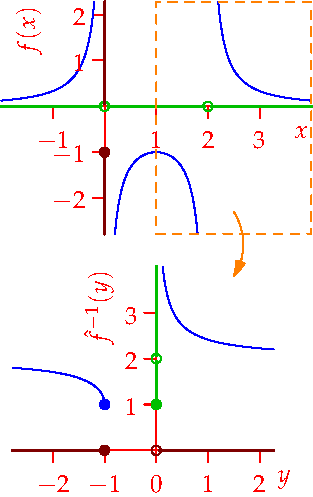
\includegraphics{dom4}
\end{example}

\goodbreak


\boldinline{Suprema and Infima}

A set $U\subseteq\R$ is \emph{bounded above} if it has an \emph{upper bound} $M$:
\[
	\exists M\in\R\text{ such that }\forall u\in U,\ u\le M
\]


\begin{axiom}{Completeness}{}
	If $U\subseteq\R$ is non-empty and bounded above, then it has a \emph{least upper bound,} the \emph{supremum} of $U$
	\[
		\sup U=\min\bigl\{M\in\R:\forall u\in U,\ u\le M\bigr\}
	\]
\end{axiom}

By convention, $\sup U:=\infty$ if $U$ is unbounded above and $\sup\emptyset:=-\infty$; now every subset of $\R$ has a supremum. Similarly, the \emph{infimum} of $U$ is its \emph{greatest lower bound}:
	\[
		\inf U=
		\begin{cases}
			\max\bigl\{m\in\R:\forall u\in U,\ u\ge m\bigr\} &\text{if $U\neq\emptyset$ is bounded below}\\
			-\infty&\text{if $U\neq\emptyset$ is unbounded below}\\
			\infty&\text{if $U=\emptyset$}
		\end{cases}
	\]
	
\begin{examples}{}{}
	Here are four sets with their suprema and infima stated. You should be able to verify these assertions directly from the definitions.
	\[
		\begin{array}{c||c|c|c|c|c}
			U&\{1,2,3,4\}&(0,5)&(-\infty,\pi]&\R&\{\frac 1n:n\in\N\}\\[2pt]\hline
			\sup U&4&5&\pi&\infty&1\\
			\inf U&1&0&-\infty&-\infty&0
		\end{array}
	\]
	Note how the supremum/infimum might or might not lie in the set itself.
\end{examples}


\boldinline{Interiors, closures, boundaries and neighborhoods}

These last concepts might not be review, but they will be used repeatedly.

\begin{defn}{}{interior}
	Let $U\subseteq\R$. A value $a\in\R$ is \emph{interior} to $U$ if it lies in some open subinterval of $U$:
	\[
		\exists\delta>0\text{ such that }(a-\delta,a+\delta)\subseteq U
	\]
	A \emph{neighborhood} of $a$ is any set to which $a$ is interior: the interval $(a-\delta,a+\delta)$ is an \emph{open $\delta$-neighborhood} of $a$. A \emph{punctured neighborhood} of $a$ is a neighborhood with $a$ deleted.\smallbreak
	The set of points interior to $U$ is denoted $U^\circ$.\smallbreak
	A \emph{limit point} of $U$ is the limit of some sequence $(x_n)\subseteq U$. The \emph{closure} $\cl U$ is the set of limit points.\smallbreak
	The \emph{boundary} of $U$ is the set $\partial U=\cl U\setminus U^\circ$.
\end{defn}

\begin{examples}{}{}
	\exstart If $U=[1,3)$, then $U^\circ=(1,3)$, \ $\cl U=[1,3]$ and $\partial U=\{1,3\}$.
	\begin{enumerate}\setcounter{enumi}{1}
	  \item $\Q^\circ=\emptyset$ and $\partial\Q=\cl\Q=\R$.
	  \item $(-3,5)\cup (5,7]$ is a punctured neighborhood of 5.
	\end{enumerate}
\end{examples}


\goodbreak
\clearpage


\setcounter{subsection}{16}
\subsection{Continuity of Functions}\label{sec:cont}

Everything in this section \emph{should} be review.

\begin{defn}{}{cont}
	A function $f:U\to\R$ is \emph{continuous at $u\in U$} if either/both of the following hold:
	\begin{enumerate}
	  \item For all sequences $(x_n)\subseteq U$ converging to $u$, the sequence $(f(x_n))$ converges to $f(u)$.
	  \item $\forall\epsilon>0$, $\exists\delta>0$ such that $(\forall x\in U)$, $\nm{x-u}<\delta\implies\nm{f(x)-f(u)}<\epsilon$.
	\end{enumerate}
	A function $f$ is \emph{continuous on $U$} if it is continuous at every point $u\in U$.
\end{defn}


\begin{examples}{}{}
	\exstart We prove that $f(x)=x^3$ is continuous at $u=2$.
	\begin{enumerate}\setcounter{enumi}{1}
		\item[]\begin{enumerate}
	  	\item (Limit method)\quad Let $x_n\to 2$. By the \emph{limit laws} (i.e. $\lim(x_n^k)=\left(\lim x_n\right)^k$),
			\[
				\lim f(x_n)=\lim x_n^3=\smash{\Bigl(\lim x_n\Bigr)^3}=2^3=f(2)
			\]
	  	\item ($\epsilon$--$\delta$ method)\quad Let $\epsilon>0$ be given and let $\displaystyle\delta=\smash{\min\left(1,\frac{\epsilon}{19}\right)}$.
			\[
				\nm{x-2}<\delta\implies \nm{x-2}<1\implies 1<x<3
			\]
			from which
			\[
				\nm{x^3-2^3}		
				=\nm{x-2}\nm{x^2+2x+2^2}
				<19\nm{x-2}\le\epsilon
			\]
			where we used the triangle inequality.
		\end{enumerate}
	
		\begin{minipage}[t]{0.70\linewidth}\vspace{0pt}
			\item Let $g(x)=
			\begin{cases}
				x\sin\frac 1x&\text{if }x\neq 0,\\
				0&\text{if }x=0
			\end{cases}$
			\smallbreak
			Then $g$ is continuous at $x=0$. Again this can be done with limits or an $\epsilon$--$\delta$ argument; both are essentially the \emph{squeeze theorem.}
	  
	  	\item The function defined by
	  	\[
	  		h(x)=
	  		\begin{cases}
	  		1+2x^2&\text{if }x<1\\
	  		2-x&\text{if }x\ge 1
	  		\end{cases}
	  	\]
	  	is discontinuous at $x=1$.
	  	\begin{enumerate}
	  		\item The sequence with $x_n=1-\frac 1n$ converges to 1, yet
				\[
					\lim h(x_n)=3\neq 1=h(1)
				\]
	   		\item Choose $\epsilon=1$ and suppose $\delta>0$ is given. Now choose $x=\max\{1-\frac\delta 2,\frac 1{\sqrt 2}\}$ to see that
				\[
					\nm{x-1}<\delta
					\quad\text{and}\quad 
					\nm{h(x)-h(1)}\ge 1=\epsilon
				\]
			\end{enumerate}
		\end{minipage}
		\hfill
		\begin{minipage}[t]{0.29\linewidth}\vspace{0pt}
			\flushright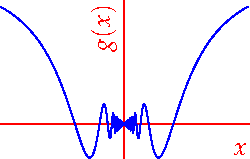
\includegraphics{cont-ex1}\bigbreak
			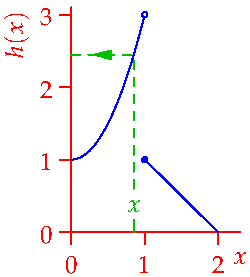
\includegraphics{cont-ex2}
		\end{minipage}
	
	
		
	% 	\begin{minipage}[t]{0.65\linewidth}\vspace{0pt}
	% 		\item We use both definitions to see that the function defined by
	%   \[h(x)=\begin{cases}
	%   1+2x^2&\text{if }x<1\\
	%   2-x&\text{if }x\ge 1
	%   \end{cases}\]
	%   is discontinuous at $x=1$.
	%   \begin{enumerate}
	%   	\item The sequence with $x_n=1-\frac 1n$ converges to 1, yet
	% 		\[\lim h(x_n)=3\neq 1=h(1)\]
	% %   	\item Choose $\epsilon=1$ and suppose $\delta>0$ is given. Choose any $x=\max\{1-\frac\delta 2,\frac 1{\sqrt 2}\}$ and observe that
	% %   	\[\nm{x-1}<\delta\quad\text{and}\quad \nm{h(x)-h(1)}\ge 1=\epsilon\]
	% 	\end{enumerate}
	% 	\end{minipage}\begin{minipage}[t]{0.35\linewidth}\vspace{0pt}
	% 	\flushright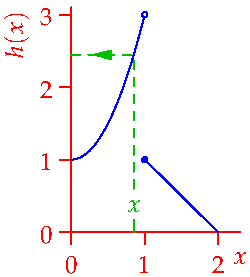
\includegraphics{cont-ex2}
	% 	\end{minipage}
	
	% 	\begin{enumerate}\setcounter{enumii}{1}
	% %   	\item The sequence with $x_n=1-\frac 1n$ converges to 1, yet
	% % 		\[\lim h(x_n)=3\neq 1=h(1)\]
	%   	\item Choose $\epsilon=1$, suppose $\delta>0$ is given, and let $x=\max\{1-\frac\delta 2,\frac 1{\sqrt 2}\}$ to observe that
	%   	\[\nm{x-1}<\delta\quad\text{and}\quad \nm{h(x)-h(1)}\ge 1=\epsilon\]
	% 	\end{enumerate}
	
	\end{enumerate} 
\end{examples}

\vfil\goodbreak


\begin{thm}{}{contdefequiv}
	The two parts of Definition \ref{defn:cont} are equivalent.
\end{thm}

\begin{proof}
	\begin{description}
		\item[\normalfont ($1\Rightarrow 2$)] We prove the contrapositive. Suppose condition 2 is \emph{false}; that is,
		\[
			\exists\epsilon>0,\text{ such that } 
			\forall\delta>0,\ \exists x\in U\text{ with } 
			\nm{x-u}<\delta\text{ and }
			\nm{f(x)-f(u)}\ge\epsilon
		\]
		In particular, for any $n\in\N$ we may let $\delta=\frac 1n$ to obtain
		\[
			\smash{\exists\epsilon>0,\text{ such that } 
			\forall n\in\N,\ \exists x_n\in U\text{ with }
			\nm{x_n-u}<\frac 1n\text{ and }
			\nm{f(x_n)-f(u)}\ge\epsilon}
		\]
		The sequence $(x_n)$ shows that condition 1 is \emph{false}:
		\begin{itemize}
	  	\item $\forall n, \ \nm{x_n-u}<\frac 1n$ whence $x_n\to u$.
	  	\item $\forall n, \ \nm{f(x_n)-f(u)}\ge\epsilon>0$, whence $f(x_n)$ \emph{does not converge to} $f(u)$.
		\end{itemize}
		
		\item[\normalfont ($2\Rightarrow 1$)] Suppose condition 2 is true, that $(x_n)\subseteq U$ converges to $u$ and that $\epsilon>0$ is given. Then
		\[
			\exists\delta>0\text{ such that }
			\nm{x-u}<\delta
			\implies \nm{f(x)-f(u)}<\epsilon
		\]
		However, by the definition of convergence ($x_n\to u$),
		\[
			\exists N\in\N \text{ such that }n>N
			\implies \nm{x_n-u}<\delta 
			\implies \nm{f(x_n)-f(u)}<\epsilon
		\]
		Otherwise said, $f(x_n)\to f(u)$.\qedhere
	\end{description}
\end{proof}

Rather than use these definitions every time, it is helpful to have a working dictionary.

\begin{thm}{Dictionary of Common Continuous Functions}{commoncont}
	\begin{enumerate}\setcounter{enumi}{0}\itemsep0pt
	  \item Suppose $f$ and $g$ are continuous at $u$ and that $k$ is constant. Then the following are continuous at $u$ (if defined---don't divide by zero!):
		\[
			f+g,\quad f-g,\quad fg,\quad \frac fg,\quad \nm f,\quad kf,\quad \max(f,g),\quad \min(f,g)
		\]
		\item If $f$ is continuous at $u$ and $h$ is continuous at $f(u)$, then $h\circ f$ is continuous at $u$.
	  \item Algebraic functions are continuous: these are functions constructed using finitely many addition/subtraction, multiplication/division and $n^\text{th}$ root operations.
		\item The familiar transcendental functions are continuous: $\exp$, $\ln$, $\sin$, etc.
	\end{enumerate}
\end{thm}


\begin{example}{}{}
	$f(x)=\sin\frac{\sqrt[3]{x^2+7}}{x-2}+\cos\frac 1{e^x-1}$ is continuous on its domain $(-\infty,0)\cup(0,1)\cup(1,\infty)$.
\end{example}


Theses claims are tedious to prove using elementary definitions. In particular, it is better to defer a proof of the transcendental claim until we can define such functions using power series, after which continuity comes for free.


\vfil\goodbreak

\begin{exercises}
	\emph{Key concepts/results:\quad Suprema/Completeness,\quad Sequential \& $\epsilon$-$\delta$ continuity}


% 	\exstart Give examples to show that $g\circ f$ being continuous can happen with:\vspace{-5pt}
	\begin{enumerate}\itemsep0pt%\setcounter{enumi}{1}  
	  \item Give examples to show that $g\circ f$ being continuous can happen with:
	  \begin{enumerate}
	    \item $f$ continuous and $g$ discontinuous. \qquad\qquad (b) \ $g$ continuous and $f$ discontinuous.
	    \item[(c)] Both $f,g$ discontinuous.
	  \end{enumerate}
	  You may use pictures, but make sure they clearly describe the functions $f,g$.
	  
	  
	  \item\begin{enumerate}
	  	\item Prove that the function $f(x)=x^3$ is continuous at $x=-2$ using an $\epsilon$--$\delta$ argument.
	  	\item Prove that $f(x)=x^3$ is continuous at $x=u$ using an $\epsilon$--$\delta$ argument.
	  \end{enumerate}
	
	
		\item Prove that the following are discontinuous at $x=0$: use \emph{both} definitions of continuity.
		\begin{enumerate}
	  	\item $f(x)=1$ for $x<0$ and $f(x)=0$ for $x\ge 0$.
	  	\item $g(x)=\sin(1/x)$ for $x\neq 0$ and $g(0)=0$.
		\end{enumerate}
		
		
		\item If $f$ is continuous at $u$, prove that it is bounded on some set $(u-\delta,u+\delta)\cap \dom(f)$.
	
	
		\item Prove the following parts of Theorem \ref{thm:commoncont} using $\epsilon$--$\delta$ arguments.
		\begin{enumerate}
	  	\item If $f,g$ are continuous at $u$, then $f-g$ is continuous at $u$.
	  	\item If $f,g$ are continuous at $u$, then $fg$ is continuous at $u$.
	  	\item If $f$ is continuous at $u$ and $h$ at $f(u)$, then $h\circ f$ is continuous at $u$.
		\end{enumerate}
	  
	  
	  \item\label{exs:isolatedcont} Suppose $f:U\to \R$ is a function whose domain $U$ contains an \emph{isolated point} $a$: i.e.\ $\exists r>0$ such that $(a-r,a+r)\cap U=\{a\}$. Prove that $f$ is continuous at $a$.
	  
	  
	  \item\label{exs:extremevaluelemma} Refresh your prerequisites by giving formal proofs:
	  \begin{enumerate}
	    \item (Suprema and sequences)\lstsp If $M=\sup U$, then $\exists (x_n)\subseteq U$ such that $x_n\to M$.\par
	    (\emph{This has to work even if $M=\infty$!})
	    \item (Limit of a bounded sequence)\lstsp If $(x_n)\subseteq[a,b]$ and $x_n\to x$, then $x\in [a,b]$.
			\item (Bolzano--Weierstraß)\lstsp Every bounded sequence in $\R$ has a convergent subsequence.\par
			(\emph{Hint: If $(x_n)\subseteq [a,b]$, explain why there exist intervals $I_1\supseteq I_2\supseteq I_3\supseteq\cdots$ such that \emph{infinitely many} $(x_n)$ lie in each interval $I_k$. Hence obtain a subsequence $(x_{n_k})$ and prove that it is \emph{Cauchy.}\footnotemark})
		\end{enumerate}
		
		
		\item (Very Hard)\lstsp Consider the function $f:\R\to\R$ where
		\[
			f(x)=
			\begin{cases}
				\frac 1q&\text{whenever }x=\frac pq\in\Q\text{ with }q>0\text{ and }\gcd(p,q)=1\\
				0&\text{ if }x\not\in\Q
			\end{cases}
		\]
	  For example, $f(1)=f(2)=f(-7)=1$, and $f(\tfrac 12)=f(-\tfrac 12)=f(\tfrac 32)=\cdots=\frac 12$, etc. Prove that $f$ is continuous at each point of $\R\setminus\Q$ and discontinuous at each point of $\Q$.
	\end{enumerate}
\end{exercises}


\footnotetext{%
	This is a good moment to review the notion of a Cauchy sequence
	\[
		\forall \epsilon>0,\exists N$ such that $m,n>N
		\implies \nm{x_m-x_n}<\epsilon
	\]
	and the discussion of Cauchy completeness: $(x_n)\subseteq\R$ is convergent if and only if it is Cauchy.%
}


\goodbreak



\subsection{Properties of Continuous Functions}\label{sec:propcont}


In this section we describe the behavior of a continuous function on an interval. We first consider the special case when the domain is a closed bounded interval $[a,b]$.

% \begin{defn}{}{}
% A function $f:U\to V$ is \emph{bounded} if $\exists M\in\R$ such that $\forall x\in U,\ \nm{f(x)}\le M$. Equivalently, both the supremum and infimum of $\range(f)$ are \emph{finite.} 
% \end{defn}


%Here is the main result:

\begin{thm}{Extreme Value Theorem}{cont2}
	A continuous function on a closed, bounded interval is bounded and attains its bounds. Otherwise said, if $f:[a,b]\to\R$ is continuous, then
	\[
		\exists x,y\in [a,b]\text{ such that }f(x)=\sup\range(f)\ \text{and}\  f(y)=\inf\range(f)
	\]
	In particular, the supremum and infimum are \emph{finite.}
\end{thm}


\begin{proof}
	Suppose $f$ is continuous with domain $[a,b]$ and let $M=\sup\{f(x):x\in[a,b]\}$. We invoke the three parts of Exercise \ref*{sec:cont}.\ref{exs:extremevaluelemma}:
	\begin{itemize}\itemsep2pt
	  \item (Part a)\lstsp There exists a sequence $(x_n)\subseteq [a,b]$ such that $f(x_n)\to M$.
	  \item (Part c)\lstsp There exists a convergent subsequence $(x_{n_k})$ with limit $x$.
	  \item (Part b)\lstsp $x\in [a,b]$.
	\end{itemize}
	Since $f$ is continuous, we now have $f(x)=\lim\limits_{k\to\infty}f(x_{n_k})=M$. This shows that $M$ is \emph{finite} and that $f$ attains its least upper bound.
	For the lower bound, apply this to $-f$.
\end{proof}
	
It is worth considering how the result can fail when one of the hypotheses is weakened. For example:
\begin{description}\itemsep0pt
	\item[\normalfont\emph{$f$ discontinuous}] $f:[0,1]\to\R:x\mapsto
	\begin{cases}
		x&\text{if }x\neq 1\\
		0&\text{if }x=1
	\end{cases}$
	is bounded but does not attain its bounds.
	\item[\normalfont\emph{$\dom(f)$ not closed}] $f:[0,1)\to\R:x\mapsto x$ is bounded but does not attain its bounds.
	\item[\normalfont\emph{$\dom(f)$ not bounded}] $f:[0,\infty)\to\R:x\mapsto x$ is unbounded.
\end{description}

\medskip


We now consider continuous functions on arbitrary intervals. The next result should be familiar from elementary calculus and is intuitively obvious from the naïve notion of continuity (draw the graph without taking your pen off the page).

\begin{thm}{Intermediate Value Theorem}{}
	Let $f:I\to\R$ be continuous on an interval $I$. Suppose $a,b\in I$ with $a<b$ and that $f(a)\neq f(b)$. If $L$ lies between $f(a)$ and $f(b)$, then $\exists \xi\in(a,b)$ such that $f(\xi)=L$.
\end{thm}


\begin{example}[lower separated=false, sidebyside, sidebyside align=top seam, sidebyside gap=0pt, righthand width=0.45\linewidth]{}{}
	Let $f(x)=\cos x$ with $a=\frac\pi 4$, $b=3\pi$ and $L=\frac 12$; then
	\[
		f(\xi)=L\iff \xi\in\left\{\frac\pi 3,\frac{5\pi}3,\frac{7\pi}3\right\}
	\]
	There may therefore be several suitable values of $\xi$. It is even possible (Exercise \ref{exs:intvalinfty}) for there to be \emph{infinitely many}.
	\tcblower
	\flushright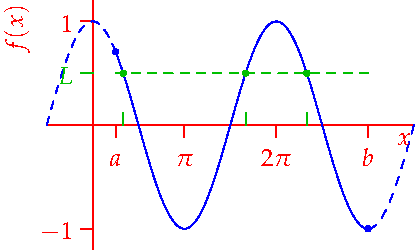
\includegraphics{intval2}
\end{example}



\begin{proof}
	Suppose WLOG that $f(a)<L<f(b)$ and let\par
	\begin{minipage}[t]{0.55\linewidth}\vspace{-15pt}
		\[
			\textcolor{Green}{S}=\{x\in[a,b]:f(x)<L\}
		\]
		Plainly $S\subseteq [a,b)$ is non-empty, hence $\xi:=\sup S$ exists and $\xi\in[a,b]$. It remains to show that $\xi$ satisfies the required properties.\medbreak
		
		By Exercise \ref{exs:extremevaluelemma}, $\exists(s_n)\subseteq S$ with $\lim s_n=\xi$.
		Since $f$ is continuous, $f(\xi)=\lim f(s_n)\le L$. In particular, $\xi\neq b$.
	\end{minipage}
	\hfill
	\begin{minipage}[t]{0.44\linewidth}\vspace{-15pt}
		\flushright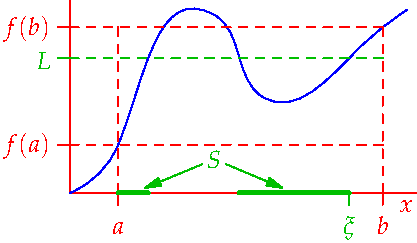
\includegraphics{intval}
	\end{minipage}
	\medbreak
	
	To finish, play a similar game with the sequence defined by $t_n=\min\{b,\xi+\frac 1n\}$ (see Exercise \ref{exs:ivtproof}).
\end{proof}


\begin{example}{}{}
	The intermediate value theorem is useful for demonstrating the existence of solutions to equations. For example, we show that the equation $x2^x=1$ has a solution.\par
	\begin{minipage}[t]{0.6\linewidth}\vspace{0pt}
		\begin{itemize}\itemsep2pt
			\item Observe that $g(x)=x2^x-1$ is continuous.
			\item $g(0)=-1<0$.
			\item $g(1)=1>0$.
			\item By the intermediate value theorem $\exists \xi\in(0,1)$ such that $g(\xi)=0$: that is $\xi\cdot 2^\xi=1$.
		\end{itemize}
	\end{minipage}
	\hfill
	\begin{minipage}[t]{0.39\linewidth}\vspace{-10pt}
		\flushright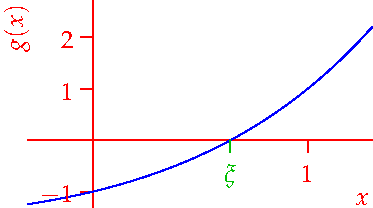
\includegraphics[scale=0.95]{intval3}
	\end{minipage}
	\bigbreak
	
	It is inefficient, but one can home in on $\xi$ by repeatedly halving the size of the interval: for instance,
	\[
		g(\tfrac 12)=\tfrac{\sqrt 2}2-1<0,\quad 
		g(\tfrac 34)=\tfrac 34\cdot 2^{3/4}-1\approx 0.26>0\ldots
		\implies \tfrac 12<\xi<\tfrac 34
	\]
\end{example}


\begin{cor}{}{}
	Continuous functions map intervals to intervals (or points).
\end{cor}

\begin{proof}
	An interval $I$ is characterized by the following property
	\[
		\forall x_1,x_2\in I,\ x\in\R,\ x_1<x<x_2\implies x\in I
	\]
	Let $f:I\to\R$ be continuous and suppose its range $f(I)$ is not a single point. If $f(a)<L<f(b)$, then $\exists \xi\text{ between $a,b$ such that }f(\xi)=L$. Otherwise said, $L\in f(I)$ and so $f(I)$ is an interval.
\end{proof}

More generally, if $\dom(f)=\bigcup I_n$ is written as a union of disjoint intervals and $f$ is continuous, then
\[
	\range(f)=\bigcup f(I_n)
\]
is also a union of intervals, though these need not be disjoint: a continuous function can bring intervals together, but cannot break them apart.\footnote{%
	More generally, if $f:U\to V$ is a continuous function between topological spaces and $a,b$ lie in the same \emph{component} of $U$, then $f(a),f(b)$ lie in the same component of $f(U)$. In our examples each component is an interval.}

\begin{example}{}{}
	The function $f(x)=\sqrt{x^2-4}$ has implied domain $(-\infty,-2]\cup[2,\infty)$ and range $[0,\infty)$. Both halves of the domain are mapped onto the same interval $\range(f)$ .
\end{example}

\goodbreak



\begin{exercises}
	\emph{Key concepts:\quad Extreme Value Theorem,\quad Intermediate Value Theorem}\vspace{-5pt}
	\begin{quote}
		\emph{Continuous functions preserve intervals}
	\end{quote}

	%\exstart Give examples of the following:\vspace{-5pt}
	\begin{enumerate}%\setcounter{enumi}{1}  
	  \item Give examples of the following:
	  \begin{enumerate}
	    \item An unbounded discontinuous function on a closed bounded interval.
	    \item An unbounded continuous function on a non-closed bounded interval.
	    \item A bounded continuous function on a closed unbounded interval which fails to attain its bounds.
		\end{enumerate}
		
	% 	\item Give an example of a discontinuous function on the interval $[0,1]$ which is not bounded. You may draw the function rather than provide a formula, provided it is clear what the function does.
	
	% 	\item Let $a<b$ be given to you. Give an example of a continuous function on $(a,b)$ which is unbounded. Give a second continuous function on $(a,b)$ which is bounded but does not attain its bounds.
		
		
		\item\label{exs:intvalinfty} Consider the function $f(x)=
		\begin{cases}
			x\sin\frac 1x&\text{if }x\neq 0\\
			0&\text{if }x=0
		\end{cases}$
		\begin{enumerate}
		  \item Explain why $f$ is continuous on any interval $I$.
		  \item Suppose $a<0<b$ and that $f(a),f(b)$ have opposite signs. If $L=0$, show that the intermediate value theorem is satisfied by \emph{infinitely many} distinct values $\xi$.
		\end{enumerate}

	
		\item Use the intermediate value theorem to prove that the equation $8x^3-12x^2-2x+1=0$ has at least 3 real solutions (and thus, by the fundamental theorem of algebra, exactly 3).
		
		
		\item\label{exs:ivtproof} Complete the proof of the intermediate value theorem by defining $t_n=\min(b,\xi+\frac 1n)$.
		
		
		\item\begin{enumerate}
		  \item Suppose $f:U\to\R$ is continuous and that $U=\bigcup\limits_{k=1}^nI_k$ is the union of a finite sequence $(I_k)$ of closed bounded intervals. Prove that $f$ is bounded and attains its bounds.
		  \item Let $U=\bigcup\limits_{n=1}^\infty I_n$, where $I_n=[\frac 1{2n},\frac 1{2n-1}]$ for each $n\in\N$. Give an example of a continuous function $f:U\to\R$ which is either unbounded or does not attain its bounds. Explain.
		\end{enumerate}
	\end{enumerate}
\end{exercises}


\clearpage


\subsection{Uniform Continuity}\label{sec:unifcont}

Recall Definition \ref{defn:cont}: $f:U\to\R$ is continuous at all points\footnote{%
	To promote symmetry, we use $y$ instead of $u$ for a generic point of $\dom(f)$.%
}
$y\in U$ provided
\[
	\forall y\in U,\ \forall\epsilon>0,\ \exists \delta>0\text{ such that }
	(\forall x\in U)\ \nm{x-y}<\delta
	\implies \nm{f(x)-f(y)}<\epsilon
\]
Note the order of the quantifiers: $\delta$ is permitted to depend \emph{both} on $y$ and $\epsilon$. In the naïve sense of continuity ($x$ close to $y\Longrightarrow f(x)$ close to $f(y)$), the meaning of \emph{close} can depend on the \emph{location} $y$. Uniform continuity is a stronger condition where the \textbf{meaning of \emph{close} is independent of location}.

\begin{defn}{}{}
	$f:U\to\R$ is \emph{uniformly continuous} if
	\[
		\forall\epsilon>0,\ \exists \delta>0\text{ such that }
		(\forall x,y\in U)\ \nm{x-y}<\delta
		\implies \nm{f(x)-f(y)}<\epsilon
	\]
\end{defn}
We've included the (typically) hidden quantifiers ($\forall x,y$) to make clear that $\delta$ is independent of $x,y$. Note also that the definition is now symmetric in $x,y$.


\begin{example}{}{unif1}
	Consider $f(x)=\frac 1x$.\par
	\begin{minipage}[t]{0.65\linewidth}\vspace{0pt}
		\begin{enumerate}
		\item If $0<a<b\le \infty$, then $f$ is uniformly continuous on $[a,b)$.\par
		Let $\epsilon>0$ be given and let $\delta=a^2\epsilon$. Then $\forall x,y\in[a,b)$,
		\[
			\nm{x-y}<\delta 
			\implies \nm{\frac 1x-\frac 1y} =\nm{\frac{y-x}{xy}}
			<\frac\delta{xy}\le\frac{\delta}{a^2}
			=\epsilon
		\]
		\item If $0<b\le\infty$, then $f$ is \emph{not} uniformly continuous on $(0,b)$.\smallbreak
		Let $\epsilon=1$ and suppose $\delta>0$ is given.\par
		Let $x=\min(\delta,1,\tfrac b2)$ and $y=\frac x2$.\par
		Certainly $x,y\in(0,b)$ and $\nm{x-y}=\frac x2\le\frac\delta 2<\delta$. However,
		\[
			\nm{f(x)-f(y)}=\frac 1x\ge 1=\epsilon
		\]
		\end{enumerate}
	\end{minipage}
	\hfill
	\begin{minipage}[t]{0.34\linewidth}\vspace{0pt}
		\flushright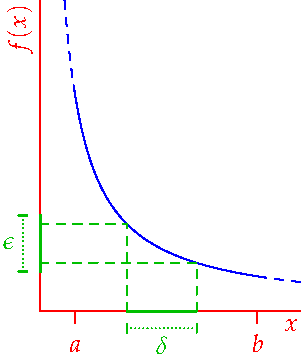
\includegraphics{unif1}
	\end{minipage}
	\bigbreak
	Think about how $\epsilon$ and $\delta$ must relate as one slides the intervals in the picture up/down and left/right.
\end{example}

Some intuition will help make sense of the example.
\begin{description}
	\item[Bounded/unbounded gradient] In part 1 $\epsilon=\delta{a^2}$, where $\frac 1{a^2}=\nm{f'(a)}$ bounds the gradient of $f$.\\
	By contrast, the slope of $f$ is \emph{unbounded} in part 2.
	\item[Extensibility] In part 1 the domain of $f$ may be extended to $a$ (and to $b$ if finite): $g:[a,b]\to\R:x\mapsto \frac 1x$ is continuous.
	In part 2, this is impossible: there is no continuous function $g:[0,b)\to\R$ such that $g(x)=\frac 1x$ whenever $x>0$.
\end{description}
Informally, if a continuous function $f$ has bounded gradient, or if you can `fill in the holes' at the endpoints of $\dom(f)$, then $f$ is uniformly continuous. When uniform continuity is used abstractly in a proof, it is often one of the above properties that is being invoked. The remainder of this section involves making these observations watertight.


\goodbreak


\begin{thm}{}{unifcontboundedslope}
	Let $f:I\to\R$ be continuous on an interval $I$ and differentiable with bounded derivative on the interior $I^\circ$. Then $f$ is uniformly continuous on $I$.
\end{thm}

The proof depends on the mean value theorem, which should be familiar from elementary calculus; we'll discuss a proof later on.

\begin{proof}
	Suppose $\nm{f'(x)}\le M$ on $I^\circ$. Let $\epsilon>0$ be given, let $\delta=\frac\epsilon M$ and suppose $(y,x)\subseteq I$. Then
	\begin{align*}
	\nm{x-y}<\delta&\implies \exists \xi\in I^\circ\text{ such that }f'(\xi)=\frac{f(x)-f(y)}{x-y} \tag{MVT}\\
	&\implies \nm{f(x)-f(y)}=\nm{f'(\xi)}\nm{x-y}<M\delta=\epsilon \tag*{\qedhere}
	\end{align*}
\end{proof}


Theorem \ref{thm:unifcontboundedslope} isn't a biconditional: for instance, Exercise \ref*{sec:unifcont}.\ref{exs:unifroots} shows that $f(x)=\sqrt x$ on $[0,\infty)$ and $g(x)=x^{1/3}$ on $\R$ are both uniformly continuous even though both have unbounded slope.\medbreak

We now discuss extensibility and how uniform continuity relates to continuity on closed sets. First we see that for closed bounded sets, uniform continuity is nothing new.

\begin{thm}{}{unifcontclosed}
	If $g:[a,b]\to\R$ is continuous, then it is uniformly continuous. 
\end{thm}

\begin{proof}
	Suppose $g$ is continuous but not uniformly so. Then
	\[
		\exists \epsilon>0\text{ such that }
		\forall\delta>0,\ \exists x,y\in [a,b]\text{ for which }
		\nm{x-y}<\delta\text{ and }
		\nm{g(x)-g(y)}\ge\epsilon \tag{$\ast$}
	\]
	For each $n\in\N$, let $\delta=\frac 1n$ to see that there exists sequences $(x_n),(y_n)\subseteq[a,b]$ satisfying the above.\\
	By Bolzano--Weierstraß, the bounded sequence $(x_n)$ has a convergent subsequence $x_{n_k}\to x\in[a,b]$. Clearly
	\[
		\nm{x_{n_k}-y_{n_k}}<\frac 1{n_k}\to 0\implies y_{n_k}\to x
	\]
	But then $\nm{g(x_{n_k})-g(y_{n_k})}\to 0$, which contradicts $(\ast)$.
\end{proof}

Now we build towards a partial converse.

\begin{lemm}{}{unifcont}
	If $f:U\to\R$ is uniformly continuous and $(x_n)\subseteq U$ is a Cauchy sequence, then $\bigl(f(x_n)\bigr)$ is also Cauchy.
\end{lemm}

\begin{proof}
	Let $\epsilon>0$ be given. Then:
	\begin{itemize}
	  \item (Uniform Continuity)\lstsp $\exists\delta>0$ such that $\nm{x-y}<\delta\Longrightarrow \nm{f(x)-f(y)}<\epsilon$.
	  \item (Cauchy)\lstsp $\exists N\in\N$ such that $m,n>N\Longrightarrow \nm{x_m-x_n}<\delta$.
	\end{itemize}
	Putting these together, we see that
	\[
		\exists N\in\N\text{ such that }m,n>N
		\implies \nm{f(x_m)-f(x_n)}<\epsilon
	\]
	Otherwise said, $\bigl(f(x_n)\bigr)$ is Cauchy.
\end{proof}
	
\goodbreak

We now see that a function $f:I\to \R$ is uniformly continuous on a bounded interval if and only it is has a \emph{continuous extension} $g:\cl I\to\R$ defined on the closure of its domain.

\begin{thm}{}{unifcontext}
	Suppose $f:I\to\R$ is continuous where $I$ is a bounded interval with endpoints $a<b$. Define $g:[a,b]\to\R$ via
	\[
		g(x)=
		\begin{cases}
	  	f(x)&\text{if }x\in I\\
	  	\lim f(x_n)&\text{whenever }(x_n)\subseteq I\text{ and }x_n\to a\\
	  	\lim f(x_n)&\text{whenever }(x_n)\subseteq I\text{ and }x_n\to b
	  \end{cases}
	 \]
	 Then $f$ is uniformly continuous if and only $g$ is well-defined ($g$ is continuous, \emph{if} well-defined).
\end{thm}

\begin{proof}
	\begin{description}
	\item[\normalfont ($\Rightarrow$)] Suppose $f$ is uniformly continuous on $I$ and that $a\not\in I$. Let $(x_n),(y_n)\subseteq I$ be sequences converging to $a$. To show that $g$ is well-defined, we must prove that $\bigl(f(x_n)\bigr)$ and $\bigl(f(y_n)\bigr)$ are convergent, and to the same limit. For this, we define a sequence
	\[
		(u_n)=(x_1,y_1,x_2,y_2,x_3,y_3,\ldots)
	\]
	Since $(x_n)$ and $(y_n)$ have the same limit $a$, we conclude that $u_n\to a$. But then $(u_n)$ is Cauchy. By Lemma \ref{lemm:unifcont}, $\bigl(f(u_n)\bigr)$ is also Cauchy and thus convergent. Since $\bigl(f(x_n)\bigr)$ and $\bigl(f(y_n)\bigr)$ are subsequences of a convergent sequence, they must also converge to the same (finite) limit.\par
	The argument when $b\not\in I$ is identical.
	\item[\normalfont ($\Leftarrow$)] If $g$ is well-defined then it is continuous (Definition \ref{defn:cont}, part 1); by Theorem \ref{thm:unifcontclosed} it is uniformly so. Since $f=g$ on a subset of $\dom(g)$, the same choice of $\delta$ will work for $f$ as for $g$: $f$ is therefore uniformly continuous.\qedhere
	\end{description}
\end{proof}


\begin{examples}{}{}
	\exstart Consider $f:x\mapsto x^2$. 
	\begin{enumerate}\setcounter{enumi}{1}
	  \item[]\begin{enumerate}
	    \item If $\dom(f)$ is the open interval $(-3,10)$, then $f$ is uniformly continuous since its derivative $f'(x)=2x$ is bounded ($\nm{f'(x)}\le 20$). The continuous extension is $g(x)=x^2$ on $[-3,10]$.
	    \item	If $\dom(f)$ is the infinite interval $(-3,\infty)$, then neither Theorem \ref{thm:unifcontboundedslope} nor \ref{thm:unifcontext} applies: both $f'$ and the domain $(-3,\infty)$ are unbounded.\par
			Instead, note that if $\epsilon=1$, then for any $\delta>0$, we can choose $x=\frac 1\delta$ and $y=\frac 1\delta+\frac\delta 2$. Clearly
			\[
				\nm{x-y}=\frac\delta 2<\delta\text{ and }
				\nm{x^2-y^2}=1+\frac{\delta^2}4>1=\epsilon
			\]
			whence $f$ is not uniformly continuous.
	  \end{enumerate}
		\item $f(x)=x\sin \frac 1x$ is continuous on the interval $(0,\infty)$. Strictly, neither Theorem \ref{thm:unifcontboundedslope} nor \ref{thm:unifcontext} apply since the derivative
		\[
			f'(x)=\sin\frac 1x-\frac 1x\cos\frac 1x
		\]
		is unbounded as is the domain. However, by breaking the domain into two pieces\ldots 
		\begin{itemize}
		  \item On $[1,\infty)$, the derivative is bounded: $\nm{f'(x)}\le 1+\frac 1{\nm x}\le 2$ by the triangle inequality. Theorem \ref{thm:unifcontboundedslope} says $f$ is uniformly continuous on $[1,\infty)$.
		  \item $f$ is continuous on $(0,1]$ and, by the squeeze theorem
		  \[
		  	x_n\to 0^+\implies \lim f(x_n)=0
		  \]
		  Extending $f$ so that $f(0)=0$ defines a continuous extension. By Theorem \ref{thm:unifcontext}, $f$ is uniformly continuous on $(0,1]$.
	 	\end{itemize}
	 	Putting this together (Exercise \ref{exs:unifcontunion}), $f$ is uniformly continuous on $(0,\infty)$. Indeed the function
	 	\[
	 		h(x)=
	 		\begin{cases}
	 			x\sin\frac 1x&\text{if }x\neq 0\\
	 			0&\text{if }x=0
	 		\end{cases}
	 	\]
	 	is uniformly continuous on $\R$.
	\end{enumerate}
\end{examples}


\begin{exercises}
	\emph{Key concepts:\quad Uniform Continuity (same $\delta$ for all locations),\quad Bounded gradient,}\vspace{-5pt}
	\begin{quote}
		\emph{Continuous extensions}
	\end{quote}
	
	%\exstart Which functions are uniformly continuous? Justify your answers.\vspace{-5pt}
	\begin{enumerate}%\setcounter{enumi}{1}  
	  \item Which functions are uniformly continuous? Justify your answers.
	  \begin{enumerate}
	    \item \makebox[200pt][l]{$f(x)=x^4$ on $[-1,1]$\hfill (b) }
	    $f(x)=x^4$ on $(-1,1]$
	    \setcounter{enumii}{2}
	    \item \makebox[200pt][l]{$f(x)=x^{-4}$ on $(0,2]$\hfill (d) }
	    $f(x)=x^{-4}$ on $(1,2]$
	    \setcounter{enumii}{4}
	    \item $f(x)=x^2\sin\frac 1x$ on $(0,1]$
	  \end{enumerate}
	  
	  
	  \item Prove that each function is uniformly continuous by verifying the $\epsilon$--$\delta$ property.
	  \begin{enumerate}
	    \item \makebox[200pt][l]{$f(x)=2x-14$ on $\R$\hfill (b) }
	    $f(x)=x^3$ on $[1,5]$
	    \setcounter{enumii}{2}
	    \item \makebox[200pt][l]{$f(x)=x^{-1}$ on $(1,\infty)$\hfill (d) }
	    $f(x)=\frac{x+1}{x+2}$ on $[0,1]$
	  \end{enumerate}
	  
	  
	  \item Prove that $f(x)=x^4$ is not uniformly continuous on $\R$.
	  
	  
	  \item\begin{enumerate}
	     \item Suppose $f$ is uniformly continuous on a bounded interval $I$. Prove that $f$ is bounded on $I$.
	     \item Use part (a) to write down a bounded interval on which the function $f(x)=\tan x$ is defined, but \emph{not} uniformly continuous.
	  \end{enumerate}
	
	
	  \item\label{exs:unifroots} Both parts of this question are easy using Exercise \ref{exs:unifcontunion}. Do them explicitly using the $\epsilon$--$\delta$ property.
	  \begin{enumerate}
	    \item Let $f(x)=\sqrt x$ with domain $[0,\infty)$. Show that $f'(x)$ is unbounded, but that $f$ is still uniformly continuous on $[0,\infty)$.\par
	    (\emph{Hint: let $\delta=(\frac\epsilon 2)^3$ and consider the cases $x\ge y\ge 0$, $x\le y\le 0$ and $x>0>y$ separately})
	    \item Prove that $g(x)=x^{1/3}$ is uniformly continuous on $\R$.\par
	    (\emph{Hint: let $\delta=\epsilon^2$ and WLOG assume $0\le y\le x$. Now compute $(\sqrt y+\epsilon)^2$\ldots })
	  \end{enumerate}


		\item\label{exs:unifcontunion} Suppose $f$ is uniformly continuous on intervals $U_1,U_2$ for which $U_1\cap U_2$ is non-empty. Prove that $f$ is uniformly continuous on $U_1\cup U_2$.\par
		(\emph{Hint: if $x,y$ do not lie in the same $U_1,U_2$, choose some $a\in U_1\cap U_2$ between $x$ and $y$})
		
	\end{enumerate}
\end{exercises}
\vfil
\goodbreak



\setcounter{subsection}{19}
\subsection{Limits of Functions}

In elementary calculus you likely saw many calculations of the following form:
\[
	\lim_{x\to 3}\frac{x^2-9}{x-3}
	=\lim_{x\to 3}\frac{(x-3)(x+3)}{x-3}
	=\lim_{x\to 3}(x+3)=6
\]
Loosely speaking, this means that if $(x_n)\subseteq\R\setminus\{3\}$ is a sequence converging to 3, then $\bigl(f(x_n)\bigr)$ converges to 6. Our goal in this section is to make this notation precise.

\begin{defn}{}{leftrightlimit}
	Suppose $f:U\to\R$, that $S\subseteq U$, and that $a$ is the limit of some sequence in $S$.\smallbreak
	We say that $L$ is the \emph{limit of $f(x)$ as $x$ tends to $a$ along $S$,}  written $\smash{\lim\limits_{x\to a^S}f(x)=L}$, provided 
	\[
		\forall (x_n)\subseteq S,\ \lim x_n=a\implies \lim f(x_n)=L
	\]
	We can now define one-sided and two-sided limits of functions:
	\begin{description}\itemsep2pt
		\item[\normalfont\emph{Right-hand limit}:] $\lim\limits_{x\to a^+}f(x)=L$ means $\exists S=(a,b)\subseteq U$ for which $\lim\limits_{x\to a^S}f(x)=L$
		\item[\normalfont\emph{Left-hand limit}:] $\lim\limits_{x\to a^-}f(x)=L$ means $\exists S=(c,a)\subseteq U$ for which $\lim\limits_{x\to a^S}f(x)=L$
		\item[\normalfont\emph{Two-sided limit}:] $\lim\limits_{x\to a}f(x)=L$ means $\exists S=(c,a)\cup(a,b)\subseteq U$ for which $\lim\limits_{x\to a^S}f(x)=L$
	\end{description}
\end{defn}

\vfil

\begin{itemize}
  \item If $U=\dom(f)$ is unbounded, then the one-sided definitions apply when $a=\pm\infty$. We omit the $\pm$ modifiers: for instance,
  \[
  	\lim_{x\to\infty}f(x)=L\iff 
  	\lim\limits_{x\to\infty^S}f(x)=L\text{ for some }
  	S=(c,\infty)\subseteq U
  \]
	\item\label{it:contlimit} Note that $f$ need not be defined at $a$, though $U=\dom(f)$ must contain at least some \emph{punctured neighborhood} of $a$ (one-sided for a one-sided limit). This will certainly happen if $U$ is a union of intervals of positive length. In such a case, one may simply replace $S$ with $U\setminus\{a\}$ in the definition: this is precisely what we did in the motivating example where $U=\R\setminus\{3\}$.\par
%   \[
%   	\lim\limits_{x\to a^{(\pm)}}f(x)=L\iff
%   	\Bigl(\forall (x_n)\subseteq U\setminus\{a\},\  \lim x_n=a
%   	\implies \lim f(x_n)=L\Bigr)
%   \]
  Moreover, in such a situation, Definition \ref{defn:cont} recovers a familiar idea from elementary calculus:
  \[
  	f \text{ is continuous at } a\in U
  	\iff f(a)=
  	\begin{cases}
  		\lim\limits_{x\to a} f(x)&\text{when }a\in U^\circ\\
  		\lim\limits_{x\to a^\pm} f(x)&\text{when }a\in U\setminus\partial U
  	\end{cases}
  	\tag{$\ast$}
 	\]
 	Warning! When $\dom(f)$ does not contain a punctured neighborhood of $a$, the right hand side doesn't exist and the assertion is \emph{false}!
  \item By modifying the proof of Theorem \ref{thm:contdefequiv} when $a,L\in\R$ are finite, we can restate using $\epsilon$-language. For instance, $\lim\limits_{x\to a}f(x)=L$ means
  \[
  	\forall\epsilon>0,\ \exists \delta>0\text{ such that }(\forall x\in\R)\ 0<\nm{x-a}<\delta\implies \nm{f(x)-L}<\epsilon
  \]
  If $a$ and/or $L$ is infinite, use the language of unboundedness: e.g. $\lim\limits_{x\to a}f(x)=\infty$ means
  \[
  	\forall M>0,\ \exists \delta>0\text{ such that }0<\nm{x-a}<\delta\implies f(x)>M
  \]
  There are \emph{fifteen} distinct combinations: \emph{three} two-sided and \emph{six} each of the one-sided limits!
\end{itemize}
\goodbreak


\begin{examples}{}{}
	\exstart Let $f(x)=\frac{2+x}x$ where $\dom(f)=U=\R\setminus\{0\}=(-\infty,0)\cup(0,\infty)$
	\begin{enumerate}\setcounter{enumi}{1}
	  \item[]	The following should be clear:
		\[
			\lim\limits_{x\to 3}f(x)=\frac 53\qquad 
			\lim\limits_{x\to \infty}f(x)=1
		\]
		To compute the first, for instance, we could choose $S=(0,3)\cup(3,\infty)$; if $(x_n)\subseteq S$ and $x_n\to 3$, then the limit laws justify the first claim
		\[
			\lim_{n\to\infty}f(x_n)=\frac{2+3}{3}=\frac 53
		\]
		as does the fact that $f$ is continuous at $x=3$. The second claim can be checked similarly.\smallbreak
		\begin{minipage}[t]{0.6\linewidth}\vspace{0pt}
		We can take one-sided limits at $x=0$:
		\[
			\lim\limits_{x\to 0^+}f(x)=\infty
			\quad\text{and}\quad
			\lim\limits_{x\to 0^-}f(x)=-\infty
		\]
		For instance, let $(x_n)\subseteq (0,\infty)$ satisfy $x_n\to 0$. Again, the limit laws show that $\lim\limits_{n\to\infty}f(x_n)=\infty$, which is enough to justify the first claim.\medbreak
		Finally, the sequences defined by $x_n=\frac 1n$ and $y_n=-\frac 1n$ both lie in $S=\R\setminus\{0\}$ and converge to zero, yet
		\[
			\lim_{n\to\infty} f(x_n)=\infty
			\neq -\infty =\lim_{n\to\infty} f(y_n)
		\]
		It follows that the two-sided limit $\displaystyle\lim\limits_{x\to 0}f(x)$ does not exist.
	\end{minipage}
	\hfill
	\begin{minipage}[t]{0.39\linewidth}\vspace{0pt}
		\flushright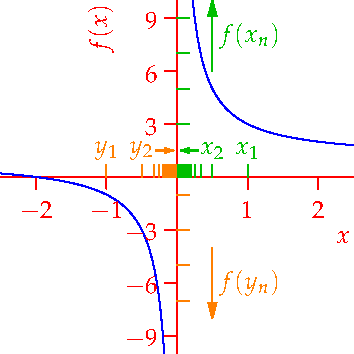
\includegraphics{limitex2}
	\end{minipage}
		
	\item Let $f(x)=\frac 1{x^2}$ whenever $x\neq 0$ and additionally let $f(0)=0$. Here the two-sided limit exists
	\[
		\lim_{x\to 0}f(x)=\infty
	\]
	However the value of the function at $x=0$ does not equal this limit: clearly $f$ is discontinuous at $x=0$.
		
	\item We revisit our motivating example. Let $f(x)=\frac{x^2-9}{x-3}$ have domain $U=\R\setminus\{3\}$. Whenever $x_n\neq 3$, we see that
	\[
		f(x_n)=\frac{(x_n-3)(x_n+3)}{x_n-3}=x_n+3
	\]
	By the limit laws, we conclude that $\lim f(x_n)=3+3=6$ and so
	\[
		\lim\limits_{x\to 3}\frac{x^2-9}{x-3}=6
	\]
	%	Implicit in the original calculation is that the function $f$ has domain \emph{excluding} 3. Indeed the original calculation relies on the following updating of the limit laws to our new context.
	\end{enumerate}
\end{examples}

\vfil
\goodbreak

Since we referenced the limit laws for sequences so often in the examples, it is appropriate to update them to this new context. We do so without proof.

\begin{cor}{Limit Laws for functions}{}
	Suppose $f,g:U\to\R$ satisfy $L=\lim\limits_{x\to a}f(x)$ and $M=\lim\limits_{x\to a}g(x)$ exist. Then,
	\begin{enumerate}
	  \item $\displaystyle\lim_{x\to a}(f+g)(x)=L+M$.
	  \item $\displaystyle\lim_{x\to a}(fg)(x)=LM$.
	  \item $\displaystyle\lim_{x\to a}\left(\frac fg\right)(x)=\frac LM$\quad (requires $M\neq 0$).
		\item If $L\in\R$ and $h$ is continuous at $L$, then $\displaystyle\lim\limits_{x\to a}(h\circ f)(x)=h(L)$.
		\item (Squeeze Theorem)\ If $L=M$ and $f(x)\le h(x)\le g(x)$ for all $x\in U$, then $\lim\limits_{x\to a}h(x)=L$.
	\end{enumerate}
	The corresponding results for one-sided limits also hold.
\end{cor}

As with the original limit laws for sequences, parts 1--3 apply provided the limits are not \emph{indeterminate forms} (e.g.\ $\infty-\infty$, $0\cdot\infty$, $\frac 00$, $\frac\infty\infty$). We'll see later how l'Hôpital's rule may be applied to such cases.


\begin{examples}{}{}
	\exstart Since $f(x)=\frac{x^2+5}{3x^2-2}$ is a rational function (continuous at all points of its domain), we quickly conclude that
	\[
		\lim\limits_{x\to 2}\frac{x^2+5}{3x^2-2}=f(2)=\frac 9{10}
	\]
	Alternatively, we may tediously invoke the other parts of the theorem:
	\begin{align*}
		\lim\limits_{x\to 2}\frac{x^2+5}{3x^2-2}
		&\overset{(3)}{=} \frac{\lim(x^2+5)}{\lim(3x^2-2)} \overset{(1)}{=} 
		\frac{\lim x^2+\lim 5}{\lim 3x^2-\lim 2} \overset{(2)}{=} 
		\frac{(\lim x)^2+5}{(\lim 3)(\lim x)^2-2}\\
		&=\frac{2^2+5}{3\cdot 2^2-2} =\frac 9{10}
	\end{align*}
	\begin{enumerate}\setcounter{enumi}{1}
		\item As $x\to\infty$, the simplistic approach results in a nonsense indeterminate form:
		\[
			\lim_{x\to\infty}\frac{x^2+5}{3x^2-2} \overset{\text{?}}{=} 
			\frac{\lim(x^2+5)}{\lim(3x^2-2)} \overset{\text{?}}{=} 
			\frac\infty\infty
		\]
		However, a little pre-theorem algebra quickly yields\footnotemark
		\[
			\lim_{x\to\infty}\frac{x^2+5}{3x^2-2} 
			=\lim_{x\to\infty}\frac{1+5x^{-2}}{3-2x^{-2}} 
			=\frac{\lim(1+5x^{-2})}{\lim(3-2x^{-2})} 
			=\frac 13
		\]
	\end{enumerate}
\end{examples}

\footnotetext{%
	Be careful! The expressions $\frac{x^2+5}{3x^2-2}$ and $\frac{1+5x^{-2}}{3-2x^{-2}}$ do not describe the same function, yet their \emph{limits} at $\infty$ are equal. The ease of equating these limits is one of the advantages of the `$\exists S$' formulation in Definition \ref{defn:leftrightlimit}. Think about why; what is a suitable set $S$ in this context?%
}

\vfil

\goodbreak


\boldsubsubsection{Classification of Discontinuities}

We now consider the ways in which a function can fail to be continuous.

\begin{defn}{}{}
	Suppose that a function is continuous on an interval except at finitely many values: we call these \emph{isolated discontinuities.}
\end{defn}

\begin{examples}{}{}
	\exstart $f(x)=\frac 1x$ has a discontinuity at $x=0$ since it is continuous on the interval $\R$, except at one point $x=0$. Note that a function need not be defined at a discontinuity!
	\begin{enumerate}\setcounter{enumi}{1}
	  \item $f(x)=\frac 1{\sin \frac 1x}$ has a \emph{non-isolated discontinuity} at $x=0$: on any interval containing zero, $f$ has infinitely many discontinuities: $x=\frac 1{\pi n}$ where $\nm n\in\N$.
	\end{enumerate}
\end{examples}


The next result helps us classify isolated discontinuities.

\begin{thm}{}{sidedlimitsequal}
	Let $f:U\to\R$ and suppose $a\in U^\circ$ is an interior point. Then
	\[
		\lim\limits_{x\to a}f(x)=L \iff \lim\limits_{x\to a^+}f(x)=L=\lim\limits_{x\to a^-}f(x)
	\]
\end{thm}

\begin{proof}
	\begin{description}
	\item[\normalfont ($\Rightarrow$)] Let $S=(c,a)\cup(a,b)$ satisfy the definition for $\lim\limits_{x\to a}f(x)=L$. Since any sequence (say) in $S^+$ is also in $S$, plainly $S^+=(a,b)$ and $S^-=(c,a)$ satisfy the one-sided definitions.
	\item[\normalfont ($\Leftarrow$)] Suppose $S^-=(c,a)$ and $S^+=(a,b)$ satisfy the one-sided definitions and denote $S=S^-\cup S^+$. Let $(x_n)\subseteq S$ be such that $x_n\to a$. Clearly $(x_n)$ is the disjoint union of two subsequences $(x_n)\cap S^+$ and $(x_n)\cap S^-$, both of which\footnotemark converge to $a$. There are three cases:%\vspace{-5pt}
	\begin{description}\itemsep0pt
		\item[$L$ \normalfont{finite}:] Let $\epsilon>0$ be given. Because of the one-sided limits,
		\begin{itemize}
	  	\item $\exists N_1$ such that $n>N_1$ and $x_n>a\implies \nm{f(x_n)-L}<\epsilon$
	  	\item $\exists N_2$ such that $n>N_2$ and $x_n<a\implies \nm{f(x_n)-L}<\epsilon$
		\end{itemize}
		Now let $N=\max(N_1,N_2)$ in the definition of limit to see that $\lim f(x_n)=L$. Since this holds for all sequences $(x_n)\subseteq S$ converging to $a$, we conclude that $\lim\limits_{x\to a}f(x)=L$.
		\item[$L=\pm\infty$:] This is an exercise.\hfill\qedhere
	
	% 	\item[$L=\infty$:] Let $M>0$ be given and repeat the above to see that $\lim f(x_n)=\infty$: the only required modification is to replace $\nm{f(x_n)-L}<\epsilon$ by $f(x)>M$,
	% 	\item[$L=-\infty$:] This is almost identical to the previous case.\hfill\qedhere
		\end{description}
	\end{description}
\end{proof}

\footnotetext{%
	It is possible for \emph{one} of these subsequences to be finite; say if $x_n>a$ for all large $n$. This is of no concern; one of the $\epsilon$-$N$ conditions would be empty and thus vacuously true.%
}


\begin{example}{}{}
	Recalling elementary calculus, we show that the following is continuous at $x=1$:
	\[
		f(x)=
		\begin{cases}
			x^2-3&\text{if }x\ge 1\\
			3-5x&\text{if }x<1
		\end{cases}
	\]
	\begin{description}
	  \item[\normalfont\emph{Step 1}:] Compute the left- and right-handed limits and check that these are equal:
	  \[
	  	\lim\limits_{x\to 1^-}f(x)=\lim\limits_{x\to 1^-}3-5x=-2,\qquad  
	  	\lim\limits_{x\to 1^+}f(x)=\lim\limits_{x\to 1^+}x^2-3=-2
	  \]
	  \item[\normalfont\emph{Step 2}:] Check that the value of the limits equals that of the function: $f(1)=1^2-3=-2$.
	\end{description}
\end{example}

\goodbreak


Recalling $(\ast)$ on page \pageref{it:contlimit}, we describe the different types of isolated discontinuity at some point $a$.
\begin{description}
	\begin{minipage}[t]{0.65\linewidth}\vspace{0pt}
	\item[Removable discontinuity] The two-sided limit $\lim\limits_{x\to a}f(x)=L$ is finite, and either:
	\begin{quote}
	  $f(a)\neq L$ or $f(a)$ is undefined.
	\end{quote}
	The term comes from the fact that we can remove the discontinuity by changing the behavior of $f$ only at $x=a$:
	\[
		\tilde f(x):=
		\begin{cases}
			f(x)&\text{if }x\neq a\\
			\lim\limits_{x\to a}f(x)&\text{if }x=a
		\end{cases}
	\]
	is now continuous at $x=a$. In the pictures,
	\[
		f_1(x)=\frac{x^2-9}{x-3}
		\quad\text{and}\quad 
		f_2(x)=
		\begin{cases}
  		x\sin(\frac 1x)&\text{if }x\neq 0\\
  		1&\text{if }x=0
  	\end{cases}
  \]
	have removable discontinuities at $x=3$ and $0$ respectively.
	\end{minipage}
	\hfill
	\begin{minipage}[t]{0.34\linewidth}\vspace{0pt}
		\flushright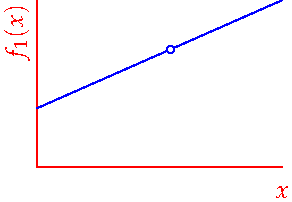
\includegraphics{discont1}\\\vfill
		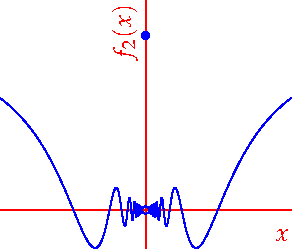
\includegraphics{discont2}
	\end{minipage}
	\smallbreak
	\begin{minipage}[t]{0.65\linewidth}\vspace{0pt}
		\item[Jump Discontinuity] The one-sided limits are finite but \emph{not equal.} A jump discontinuity cannot be removed by changing or inserting a value at $x=a$. The picture shows
		\[
			g(x)=\frac{\nm x}x=
			\begin{cases}
				1&\text{if }x>0\\
				-1&\text{if }x<0
			\end{cases}
		\]
		with a jump discontinuity at $x=0$.
	\end{minipage}
	\hfill
	\begin{minipage}[t]{0.34\linewidth}\vspace{0pt}
		\flushright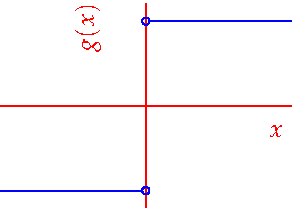
\includegraphics{discont3}
	\end{minipage}
	\smallbreak
	\begin{minipage}[t]{0.65\linewidth}\vspace{0pt}
		\item[Infinite discontinuity] The one-sided limits exist but at least one is infinite. We call the line $x=a$ a  \emph{vertical asymptote.} The picture shows
		\[
			h(x)=\frac 1{x^2}
		\]
		with an infinite discontinuity $x=0$. The fact that the one-sided limits of $h$ are equal (and infinite) is irrelevant.
	\end{minipage}
	\hfill
	\begin{minipage}[t]{0.34\linewidth}\vspace{0pt}
		\flushright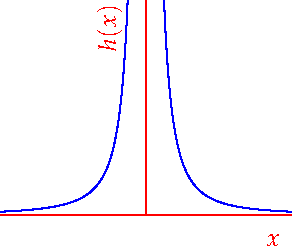
\includegraphics{discont4}
	\end{minipage}
	\smallbreak
	\begin{minipage}[t]{0.65\linewidth}\vspace{0pt}
		\item[Essential discontinuity] At least one of the one-sided limits does not exist. The picture shows $j(x)=\sin\frac 1x$ for which neither of the limits $\lim\limits_{x\to 0^\pm}j(x)$ exist.
	\end{minipage}
	\hfill
	\begin{minipage}[t]{0.34\linewidth}\vspace{0pt}
		\flushright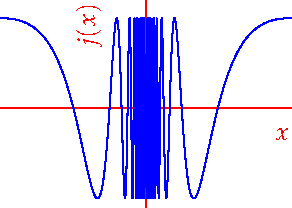
\includegraphics{discont5}
	\end{minipage}
\end{description}
It is also reasonable to refer to removable, infinite or essential discontinuities at interval endpoints.

\clearpage

\begin{exercises}
	\emph{Key concepts:\quad $\lim\limits_{x\to a}f(x)=L$,\quad $\epsilon,\delta,M,N$  versions,\quad Limit Laws,\quad Discontinuities}


	%\exstart For the function $f(x)=\frac{x^3}{\nm x}$, determine the limits $\lim\limits_{x\to\infty}f(x)$, $\lim\limits_{x\to-\infty}f(x)$, $\lim\limits_{x\to 0^-}f(x)$, $\lim\limits_{x\to 0^+}f(x)$ and $\lim\limits_{x\to 0}f(x)$, if they exist.
	
	\begin{enumerate}\itemsep0pt%\setcounter{enumi}{1}\itemsep0pt 
	  \item Given $f(x)=\frac{x^3}{\nm x}$, find $\lim\limits_{x\to\infty}f(x)$, $\lim\limits_{x\to-\infty}f(x)$, $\lim\limits_{x\to 0^-}f(x)$, $\lim\limits_{x\to 0^+}f(x)$ and $\lim\limits_{x\to 0}f(x)$, if they exist.
	  
	  \item Evaluate the following limits \emph{using the methods of this section}
	  \begin{enumerate}
	    \item \makebox[140pt][l]{$\displaystyle\lim_{x\to a}\frac{\sqrt x -\sqrt a}{x-a}$\hfill(b)}
	    \space$\displaystyle\lim_{x\to a}\frac{x^{-3/2}-a^{-3/2}}{x-a}$
	    \item[(c)] \makebox[140pt][l]{$\displaystyle\lim\limits_{x\to 0}\frac{\sqrt{1+3x^2}-1}{x^2}$\hfill(d)}
	    \space $\displaystyle\lim\limits_{x\to -\infty}\frac{\sqrt{4+3x^2}-2}{x}$
	  \end{enumerate}
	  
	 	%\item Evaluate the limits $\textstyle\lim\limits_{x\to 0}\frac{\sqrt{1+3x^2}-1}{x^2}$. Justify all your steps.
	  
	  \item Suppose that the limits $L=\lim\limits_{x\to a^+}f(x)$ and $M=\lim\limits_{x\to a^+}g(x)$ exist.
	  \begin{enumerate}
	    \item Suppose $f(x)\le g(x)$ for all $x$ in some interval $(a,b)$. Prove that $L\le M$.
	    \item Do we have the same conclusion if we have $f(x)<g(x)$ on $(a,b)$, or can we conclude that $L<M$? Prove your assertion, or give a counter-example.
	  \end{enumerate}
	  
	  
	  \item Suppose that $\lim\limits_{x\to\infty}f(x)=\lim\limits_{x\to\infty}g(x)=\infty$. Using \emph{only} this information, which of the following can you evaluate? Prove your assertions in each case.
	  \begin{enumerate}
	    \item $\lim\limits_{x\to\infty}(f+g)(x)$\qquad
			(b) \ $\lim\limits_{x\to\infty}(f-g)(x)$\qquad
			(c) \ $\lim\limits_{x\to\infty}(fg)(x)$\qquad
			(d) \ $\lim\limits_{x\to\infty}(f/g)(x)$
	  \end{enumerate}
	  
	  
	  \item Complete the proof of Theorem \ref{thm:sidedlimitsequal} by considering the $L=\pm\infty$ cases.
	  
	  
	  \item Graph $f:\R\to\R$, find and identify the types of its discontinuities.
	  \[
	  	f(x)=
	  	\begin{cases}
	    	0&x=0,\pm 1\\
	      \frac x{\nm x}&0<\nm x<1\\
	      x^2&\nm x>1
	    \end{cases}
	  \]
	  
	  
	  \item Find the discontinuities and identify their types for the following function
	  \[
	  	f(x)=
	  	\begin{cases}
	  		\frac 1x\sin\frac 1x&\text{if $x<0$ or $x>1$}\\
	  		\frac 1x&\text{if }0<x\le 1
	  	\end{cases}
	  \]
	  
	  
	  \item Let $a\in U^\circ$. Verify the claim following Definition \ref{defn:leftrightlimit}: $\lim\limits_{x\to a}f(x)=L$ if and only if
	  \[
	  	\forall\epsilon>0,\exists\delta>0\text{ such that }0<\nm{x-a}<\delta\implies \nm{f(x)-L}<\epsilon
	  \]
	  
	  
	  \item Recall Exercise \ref*{sec:cont}.\ref{exs:isolatedcont}, where we saw that a function $f:U\to\R$ is continuous at any isolated point $a\in U$.
	  \begin{enumerate}
	    \item Any function with domain $\dom(f)=\Z$ is continuous everywhere! Explain why we cannot define any limits $\lim\limits_{x\to a^{(\pm)}}f(x)$ for such a function.\par
	    (\emph{Hint: Being unable to define a limit is different from saying $\lim f(x)=\text{DNE}$: see page \pageref{it:contlimit}.})
	    \item Suppose $g(x)=x^2h(x)$ has $\dom(g)=\{0\}\cup\{\tfrac 1n:n\in\Z\}$, where $h$ is any function taking values in the interval $[-1,1]$. Explain why $g$ is continuous at every point of its domain.
		\end{enumerate}
		(\emph{These awkward examples of continuity can be avoided if we follow our usual approach where a domain is a union of intervals of positive length. This restriction is essentially baked in to the Definition \ref{defn:leftrightlimit}.})
	  
	\end{enumerate}
\end{exercises}
\graphicspath{{2series/asy/}}

\section{Sequences and Series of Functions}

If $(f_n)$ is a sequence of functions, what should we mean by $\lim f_n$? This question is of huge relevance to the history of calculus: Issac Newton's work in the late 1600's made great use of \emph{power series,} which are naturally constructed as limits of sequences of polynomials.\medbreak
For instance, for each $n\in\N_0$, we might consider the polynomial function $f_n:\R\to\R$ defined by
\[
	f_n(x)=\sum_{k=0}^nx^k=1+x+\cdots+x^n
\]
This is easily differentiated and integrated using the power law. What, however, are we to make of the \emph{series}
\[
	f(x):=\sum_{n=0}^\infty x^n=1+x+x^2+\cdots\ \text{?}
\]
Does this make sense as a function? What is its domain? Does it equal the limit of the sequence $(f_n)$ in any meaningful way? Is it continuous, differentiable, integrable? If so, can we compute its derivative or integral term-by-term: for instance, is it legitimate to write
\[
	f'(x)=\sum_{n=1}^\infty nx^{n-1}=1+2x+3x^2+\cdots\ \text{?}
\]
To many in Newton's time, such technical questions were less important than the application of calculus to the natural sciences. For the 18\th{} and 19\th{} century mathematicians who followed, however, the widespread application of calculus only increased the imperative to rigorously address these issues. 


\setcounter{subsection}{22}
\subsection{Power Series}

First we review some of the important definitions, examples and results concerning infinite series.

\begin{defn}{}{}
	Let $(b_n)_{n=m}^\infty$ be a sequence of real numbers. The \emph{(infinite) series} $\sum b_n$ is the limit of the sequence $(s_n)$ of \emph{partial sums},
	\[
		s_n=\sum_{k=m}^nb_n=b_m+b_{m+1}+\cdots+b_n,\qquad 
		\sum_{n=m}^\infty b_n=\lim_{n\to\infty}s_n
	\]
	The series $\sum b_n$ is said to \emph{converge}, \emph{diverge to infinity} or \emph{diverge by oscillation\footnotemark} as does $(s_n)$.\smallbreak
	$\sum b_n$ is \emph{absolutely convergent} if $\sum\nm{b_n}$ converges. A convergent series that is not absolutely convergent is \emph{conditionally convergent}.
\end{defn}

\footnotetext{%
	Recall that every sequence $(s_n)$ has subsequences tending to each of 
	\[
		\limsup s_n=\lim_{N\to\infty}\sup\{x_n:n>N\}\quad\text{and}\quad 
		\liminf s_n=\lim_{N\to\infty}\inf\{x_n:n>N\}
	\]
	If $(s_n)$ converges, or diverges to $\pm\infty$, then $\lim s_n=\limsup s_n=\liminf s_n$. The remaining case, divergence by oscillation, is when $\liminf s_n\neq\limsup s_n$: there exist (at least) two subsequences tending to different limits.
}


\goodbreak


\begin{examples}{}{}
	These examples form the standard reference dictionary for analysis of more complicated series. Make sure they are familiar!\textsuperscript{\ref{fn:seriesexs}}\vspace{-10pt}
	\addtocounter{footnote}{1}%\footnotemark[\value{footnote}]{}
	\begin{enumerate}\itemsep0pt
	  \item (Geometric series)\quad If $r$ is constant, then $s_n=\sum\limits_{k=0}^n r^k=\frac{1-r^{n+1}}{1-r}$.
	  It follows that
	  \[
	  	\sum_{n=0}^\infty r^n\quad  
	  	\begin{cases}
	  		\text{converges (absolutely) to }\frac 1{1-r}&\text{if }-1<r<1\\
	  		\text{diverges to }\infty&\text{if }r\ge 1\\
	  		\text{diverges by oscillation}&\text{if }r\le -1
	  	\end{cases}
	  \]
	  \item (Telescoping series)\quad If $b_n=\frac 1{n(n+1)}$, then $s_n=\sum\limits_{k=1}^nb_n =1-\frac 1{n+1}\implies \sum\limits_{n=1}^\infty\frac 1{n(n+1)}=1$.
	  \item $\sum\limits_{n=1}^\infty \frac 1{n^2}$ is (absolutely) convergent. In fact $\sum\limits_{n=1}^\infty\frac 1{n^2}=\frac{\pi^2}6$, though checking this explicitly is tricky.
	  \item (Harmonic series)\quad $\sum\limits_{n=1}^\infty\frac 1n$ is divergent to $\infty$.
		\item (Alternating harmonic series)\quad $\sum\limits_{n=1}^\infty \frac{(-1)^n}n$ is conditionally convergent.
	\end{enumerate}
\end{examples}


\footnotetext[\value{footnote}]{\label{fn:seriesexs}
	We give sketch proofs or refer to a standard `test.' Review these if you are unfamiliar.
	\begin{enumerate}
	  \item $s_n-rs_n=1+r+\cdots+r^n-(r+\cdots +r^n+r^{n+1})=1-r^{n+1}\Longrightarrow s_n=\frac{1-r^{n+1}}{1-r}$.
	  \item By partial fractions, $b_n=\frac 1n-\frac 1{n+1}\Longrightarrow s_n=\left(1-\frac 12\right)+\left(\frac 12-\frac 13\right)+\cdots+\left(\frac 1n-\frac 1{n+1}\right)=1-\frac 1{n+1}$.
	  \item Use the comparison or integral tests. Alternatively: For each $n\ge 2$, we have $\frac 1{n^2}<\frac 1{n(n-1)}$. By part 2,
	  \[
	  	s_n=\sum_{k=1}^n\frac 1{k^2}<1+\sum_{k=1}^n\frac 1{k(k-1)}<1+\sum_{n=1}^\infty\frac 1{n(n-1)}=2
	  \]
	  Since $(s_n)$ is monotone-up and bounded above by 2, we conclude that $\sum\frac 1{n^2}$ is convergent.
	  \item Use the integral test. Alternatively, observe that
	  \[
	  	s_{2^{n+1}}-s_{2^n}=\sum_{k=2^n-1}^{2^{n+1}}\frac 1k\ge\frac{2^n}{2^{n+1}}=\frac 12 \Longrightarrow s_{2^n}\ge\frac n2\xrightarrow[n\to\infty]{}\infty
	  \]
	  Since $s_n=\sum\limits_{k=1}^n\frac 1k$ is monotone-up, we conclude that $s_n\to\infty$.
	  \item Use the alternating series test, or explicitly check that both the even and odd partial sums $(s_{2n})$ and $(s_{2n+1})$ are convergent (monotone and bounded) to the same limit (essentially the proof of the alternating series test).
	\end{enumerate}
	Root Test: $\beta<1\Longrightarrow\exists \epsilon>0$ such that $\nm{b_n}^{1/n}\le 1-\epsilon$ (for large $n$) $\Longrightarrow\sum\nm{b_n}$ converges by comparison with $\sum(1-\epsilon)^n$.\smallbreak
	$\beta>1\Longrightarrow$ some subsequence of $(\nm{b_n}^{1/n})$ converges to $\beta>1\Longrightarrow b_n\nrightarrow 0\Longrightarrow \sum b_n$ diverges ($n$\th-term test).
}

% \begin{thm}{Comparison Test/Absolute Convergence}{}
% Suppose $\nm{b_n}\le a_n$ for all large $n$. Then
% \begin{itemize}
%   \item $\sum a_n$ convergent $\implies \sum b_n$ convergent. Taking $a_n=\nm{b_n}$ says that absolute convergence implies convergence.
%   \item \sum 
% \end{itemize}
% \end{thm}


\begin{thm}{Root Test}{roottest}
	Given a series $\sum b_n$, let $\beta=\limsup\nm{b_n}^{1/n}$,
	\begin{itemize}%\itemsep0pt
	  \item If $\beta<1$ then the series converges absolutely.
	  \item If $\beta>1$ then the series diverges.
	\end{itemize}
\end{thm}

\goodbreak


The root test is inconclusive if $\beta=1$. Some simple inequalities\footnote{%
	You should have encountered these previously: $\liminf\nm{\frac{b_{n+1}}{b_n}}\le \liminf\nm{b_n}^{1/n}\le \limsup\nm{b_n}^{1/n} \le\limsup\nm{\frac{b_{n+1}}{b_n}}$%
}
yield a test that is often easier to apply.

\begin{cor}{Ratio Test}{ratiotest}
	Given a series $\sum b_n$:
	\begin{itemize}\itemsep0pt
	  \item If $\limsup\nm{\frac{b_{n+1}}{b_n}}<1$ then $\sum b_n$ converges absolutely.
	  \item If $\liminf\nm{\frac{b_{n+1}}{b_n}}>1$ then $\sum b_n$ diverges.
	\end{itemize}
\end{cor}

We are now ready to properly define and analyze our main objects of interest.

\begin{defn}{}{}
	A \emph{power series centered at $c\in\R$} with \emph{coefficients} $a_n\in\R$ is a formal expression
	\[
		\sum_{n=m}^\infty a_n(x-c)^n
	\]
	where $x\in\R$ is considered a variable. A power series is a \emph{function} whose implied domain is the set of $x$ for which the resulting infinite series converges. 
\end{defn}

It is common to refer simply to a \emph{series}, and modify by infinite/power only when clarity requires. Almost always $m=0$ or 1, and it is common for examples to be centered at $c=0$.


\begin{example}{}{ps1}
	By the geometric series formula,
	\begin{gather*}\label{ex:bob}
		\textcolor{blue}{\sum_{n=0}^\infty \frac{(-1)^n}{2^n}(x-4)^n}=\frac 1{1-\frac{-(x-4)}2} 
		=\textcolor{Green}{\frac 2{x-2}} \quad
		\text{whenever}\quad\nm{-\frac{x-4}2}<1\iff 2<x<6
	\end{gather*}
	\begin{minipage}[t]{0.62\linewidth}\vspace{0pt}
	The \textcolor{blue}{series} is valid (converges) only on the subinterval $(2,6)$ of the implied domain of the \textcolor{Green}{function} $x\mapsto \frac 2{x-2}$.\par
	The behavior as $x\to 2^+$ is unsurprising, since evaluating the power series results in the divergent infinite series
	\[
		\sum 1=+\infty
	\]
	By contrast, as $x\to 6^-$ we see that limits and infinite series do not interact as we might expect,
	\begin{gather*}
		\lim\limits_{x\to 6^-}\sum_{n=0}^\infty \frac{(-1)^n}{2^n}(x-4)^n=\lim\limits_{x\to 6^-}\frac 2{x-2}=\frac 12\\
		\sum_{n=0}^\infty \lim\limits_{x\to 6^-}\frac{(-1)^n}{2^n}(x-4)^n =\sum (-1)^n =\text{DNE}
	\end{gather*}
	with the last series being divergent by oscillation.
	\end{minipage}
	\hfill
	\begin{minipage}[t]{0.37\linewidth}\vspace{0pt}
		\flushright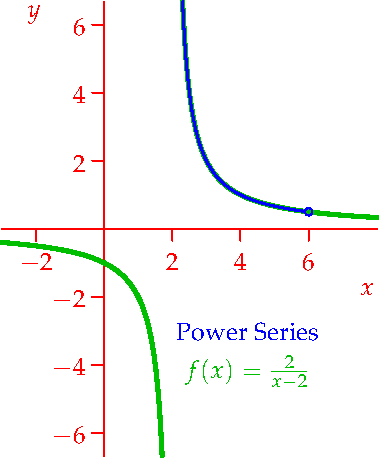
\includegraphics[scale=0.95]{powerseriesex}
	\end{minipage}
\end{example}

The example shows that we cannot blindly take limits inside an infinite sum; understanding precisely when this is possible is one of our primary goals. 


\goodbreak


\boldsubsubsection{Radius and Interval of Convergence}

The implied domain of the series in Example \ref{ex:ps1} turned out to be an \emph{interval} $(2,6)$. Somewhat amazingly, the root test (Theorem \ref{thm:roottest}) shows that the same is true for \emph{every} power series!

\begin{thm}{Root Test for Power Series}{seriesconv}
	Given a power series \smash[b]{$\sum a_n(x-c)^n$,} define\footnotemark
	\[
		R=\frac 1{\limsup\nm{a_n}^{1/n}}
	\]
	The precisely one of the following statements holds:
	\[
		\begin{array}{@{}ll}
			R\in(0,\infty)&\text{the series converges absolutely when $\nm{x-c}<R$ and diverges when $\nm{x-c}>R$}\\[5pt]
			R=\infty&\text{the series converges absolutely for all $x\in\R$}\\[5pt]
			R=0&\text{the series converges only at the center $x=c$}
		\end{array}
	\]
\end{thm}

\footnotetext{%
	Since $\nm{a_n}\ge 0$, we here adopt the conventions $\frac 10=\infty$, $\frac 1\infty=0$. With similar caveats, one can write $R=\liminf\nm{a_n}^{-1/n}$. Since every sequence has a limit superior, this really is a \emph{definition.} Whether one can easily \emph{compute} $R$ is another matter\ldots%
}

\begin{proof}
	For each fixed $x\in\R$, let $b_n=a_n(x-c)^n$ and apply the root test to $\sum b_n$, noting that
	\begin{gather*}
		\limsup\nm{b_n}^{1/n}=
		\begin{cases}
			\limsup\nm{a_n}^{1/n}\nm{x-c}=\frac 1R\nm{x-c}&\text{if $R\in(0,\infty)$}\\
			0&\text{if }R=\infty\text{ or }x=c\\
			\infty&\text{if }R=0\text{ and }x\neq c
		\end{cases}
	\end{gather*}
	In the first situation, $\limsup\nm{b_n}^{1/n}<1\iff \nm{x-c}<R$, etc.
\end{proof}

\begin{defn}{}{}
	The \emph{radius of convergence} is the value $R$ defined in Theorem \ref{thm:seriesconv}. The \emph{interval of convergence} is the set of $x\in\R$ for which the series converges; its implied domain.
	\[
		\begin{array}{c|c}
			\text{Radius of convergence}&\text{Interval of convergence}\\\hline\hline
			R\neq 0,\infty&(c-R,c+R),\ (c-R,c+R],\ [c-R,c+R)\ \text{or }[c-R,c+R]\\
			\infty&\R=(-\infty,\infty)\\
			0&\{c\}
		\end{array}
	\]
	In the first case, convergence/divergence at the endpoints of the interval of convergence must be tested for separately.
\end{defn}

The ratio test (Corollary \ref{cor:ratiotest}) provides a more user-friendly version.

\begin{cor}{Ratio Test for Power Series}{ratiops}
	If the limit exists, $R=\lim\limits_{n\to\infty}\nm{\frac{a_n}{a_{n+1}}}$.
\end{cor}

The ratio test is \emph{weaker} than the root test: as Example \ref*{ex:easyintconv}.\ref{ex:easyintconv2} shows, there exist series for which the ratio test is be inconclusive.

\goodbreak


\begin{examples}{}{easyintconv}
	\exstart The series $\sum_{n=1}^\infty \frac 1nx^n$ is centered at $0$. The ratio test tells us that
	\begin{enumerate}\setcounter{enumi}{1}
	  \begin{minipage}[t]{0.65\linewidth}\vspace{-15pt}
	  \item[]
	  \[
	  	R=\lim_{n\to\infty}\nm{\frac{a_n}{a_{n+1}}}
	  	=\lim_{n\to\infty}\frac{1/n}{1/(n+1)} 
	  	=\lim_{n\to\infty}\frac{n+1}{n}=1
	  \]
	  Test the endpoints of the interval of convergence separately:
	  \[
	  	\begin{array}{ll}
	  		x=1&\sum \frac 1n=\infty\text{ diverges}\\[5pt]
	  		x=-1&\sum \frac{(-1)^n}n\text{ converges (conditionally)}
	  	\end{array}
	  \]
	  We conclude that the interval of convergence is $[-1,1)$.\medbreak
	  It can be seen (later) that the series converges to \textcolor{Green}{$-\ln(1-x)$} on its interval of convergence. As in Example \ref{ex:ps1}, this function has a larger domain $(-\infty,-1)$, than that of the \textcolor{blue}{series}.
		\end{minipage}
		\hfill
		\begin{minipage}[t]{0.34\linewidth}\vspace{0pt}
			\flushright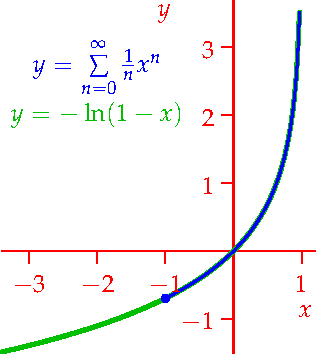
\includegraphics[scale=0.95]{powerseriesex2}
		\end{minipage}
		
		
	  \item The series $\sum_{n=1}^\infty\frac 1{n^2}x^n$ similarly has
	  \[
	  	R=\lim_{n\to\infty}\nm{\frac{a_n}{a_{n+1}}}
	  	=\lim_{n\to\infty}\frac{(n+1)^2}{n^2}=1
	  \]
		Since $\sum \frac 1{n^2}$ is absolutely convergent, we conclude that the power series also converges absolutely at $x=\pm 
		1$; the interval of convergence is $[-1,1]$.
	
		\item The series $\sum_{n=0}^\infty \frac 1{n!}x^n$ converges absolutely for all $x\in\R$, since
	  \[
	  	R=\lim_{n\to\infty}\nm{\frac{a_n}{a_{n+1}}}
	  	=\lim_{n\to\infty}\frac{(n+1)!}{n!}
	  	=\lim_{n\to\infty}(n+1)=\infty
	  \]
	  You should recall from elementary calculus that this series converges to the natural exponential function $\exp(x)=e^x$ everywhere on $\R$; indeed this is one of the common \emph{definitions} of the exponential function.
	
	
		\item The series $\sum_{n=0}^\infty n!x^n$ has $R=\lim\frac{n!}{(n+1)!}=0$. It therefore converges only at its center $x=0$.
	
	
		\item\label{ex:easyintconv2} Let $a_n=\left(\frac 23\right)^n$ if $n$ is even and $\left(\frac 32\right)^n$ if $n$ is odd. If we try to apply the ratio test to the series $\sum_{n=0}^\infty a_nx^n$, we see that
		\[
			\nm{\frac{a_n}{a_{n+1}}}=
			\begin{cases}
				\left(\frac 23\right)^{2n+1}&\text{if $n$ even}\\
				\left(\frac 32\right)^{2n+1}&\text{if $n$ odd}
			\end{cases}
			\implies \limsup\nm{\frac{a_n}{a_{n+1}}}
			=\infty\neq 0=\liminf\nm{\frac{a_n}{a_{n+1}}}
		\]
		The ratio test is therefore inconclusive. However, by the root test,
		\[
			\nm{a_n}^{1/n}=
			\begin{cases}
				\frac 23&\text{if $n$ even}\\
				\frac 32&\text{if $n$ odd}
			\end{cases}\ 
			\implies R=\frac 1{\limsup\nm{a_n}^{1/n}}=\frac 1{3/2}=\frac 23
		\]
		It is easy to check that the series diverges at $x=\pm\frac 23$; the interval of convergence is $(-\frac 23,\frac 23)$.
	\end{enumerate}
\end{examples}
\goodbreak

With the help of the root test the domain of a power series is fully understood. Limits, continuity, differentiability and integrability are more delicate. We will return to these once we've developed some of the ideas around \emph{convergence} for \emph{sequences of functions.}

\goodbreak

\begin{exercises}
	\emph{Key concepts:\quad Power Series,\quad Radius/interval of convergence $R=\frac 1{\limsup\nm{a_n}^{1/n}}$}
	
	\begin{enumerate}
		\item For each power series, find the radius and interval of convergence:
		\begin{enumerate}
		  \item \makebox[120pt][l]{$\displaystyle\sum\frac{(-1)^n}{n^24^n}x^n$\hfill(b) }\
			\makebox[140pt][l]{$\displaystyle\sum\frac{(n+1)^2}{n^3}(x-3)^n$\hfill(c) }\
			$\displaystyle\sum\sqrt nx^n$
			\item[(d)] \makebox[120pt][l]{$\displaystyle\sum\frac{1}{n^{\sqrt n}}(x+7)^n$\hfill(e) }\
			\makebox[140pt][l]{$\displaystyle\sum (x-\pi)^{n!}$\hfill(f) }\
			$\displaystyle\sum\frac{3^n}{\sqrt n}x^{2n+1}$
		\end{enumerate}
	  
	  
	  \item For each $n\in\N$ let $a_n=\left(\frac{4+2(-1)^n}{5}\right)^n$
	  \begin{enumerate}
	    \item Find $\limsup\nm{a_n}^{1/n}$, $\liminf\nm{a_n}^{1/n}$, $\limsup\nm{\frac{a_{n+1}}{a_n}}$ and $\liminf\nm{\frac{a_{n+1}}{a_n}}$.
	    \item Does the series $\sum a_n$ converge? What about $\sum (-1)^na_n$? Why?
	    \item Find the interval of convergence of the power series $\sum a_nx^n$.
	  \end{enumerate}
	  
	  
	  \item Suppose that $\sum a_nx^n$ has radius of convergence $R$. If $\limsup\nm{a_n}>0$, prove that $R\le 1$.
	  
	  
	  \item On the interval $(-\frac 23,\frac 23)$, express the series in Example \ref*{ex:easyintconv}.\ref{ex:easyintconv2} as a simple function.\par
	  (\emph{Hints: Use geometric series formulæ and the fact that the value of an absolutely convergent series is independent of rearrangements}) 
	  
	  
		\item Consider the power series
		\[
			\sum_{n=1}^\infty \frac{1}{3^nn}(x-7)^{5n+1} 
			=\frac 13(x-7)+\frac 1{18}(x-7)^6+\frac 1{81}(x-7)^{11}+\cdots 
		\]
		Since only one in five of the terms are non-zero, it is a little tricky to analyze using a naïve application of our standard tests.
		\begin{enumerate}
		  \item Explain why the ratio test for power series (Corollary \ref{cor:ratiops}) does not apply.
		  
		  \item Writing the series as $\sum a_m(x-7)^m$, observe that
		  \begin{gather*}
				a_m=\begin{cases}
				\frac 5{3^{\frac{m-1}5}(m-1)}&\text{if $m\equiv 1\mod 5$}\\
				0&\text{otherwise}
			\end{cases}%\\
			%\implies \limsup\nm{a_m}^{1/m} = \lim\frac{5^{1/m}}{3^{\frac 15-\frac 1{5m}}(m-1)^{1/m}} =3^{-1/5} \implies R=\sqrt[5]{3}
			\end{gather*}
		  Use the root test (Theorem \ref{thm:seriesconv}) and your understanding of elementary limits to directly compute the radius of convergence.
		  
		  \item Alternatively, write $\sum \frac{1}{3^nn}(x-7)^{5n+1}=\sum b_n$. Apply the ratio test for \emph{infinite} series (Corollary \ref{cor:ratiotest}): what do you observe? Use your observation to compute the radius of convergence of the original series in a simpler manner than part (a).
		  
		  \item Finally, check the endpoints to determine the interval of convergence.
		\end{enumerate}
		
		%\item Find the interval of convergence of the series $\sum 2^n(2x-1)^{2n}$
	\end{enumerate}
\end{exercises}


\clearpage
\iffalse


\subsection{Uniform Convergence}\label{sec:uniformconv}

In this section we consider sequences $(f_n)$ of \emph{functions} $f_n:U\to\R$ and their limits.

\begin{example}{}{seqfn}
	For each $n\in\N$, define $f_n:(0,1)\to\R:x\mapsto x^n$. Several examples are graphed.
	\begin{center}
		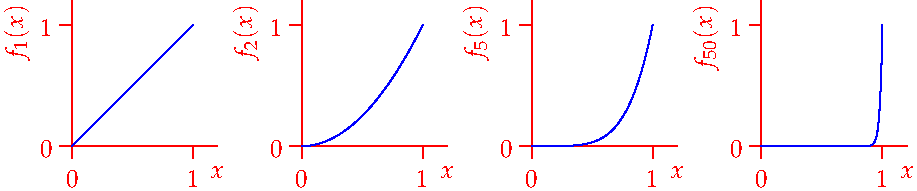
\includegraphics{seqex1}
	\end{center}
\end{example}

There are several useful notions of convergence for sequences of functions. The simplest is where, for each $x$, $(f_n(x))$ is treated as a separate sequence of real numbers.\goodbreak

\begin{defn}{}{}
Suppose a function $f$ and a sequence of functions $(f_n)$ are given. We say that \emph{$(f_n)$ converges pointwise to $f$ on $U$} if,
\[\forall x\in U,\ \lim\limits_{n\to\infty}f_n(x)=f(x)\]
\end{defn}

It is common to write `$f_n\to f$ pointwise.' For reference, we state two equivalent rephrasings:
\begin{enumerate}
  \item $\displaystyle \forall x\in U, \ \nm{f_n(x)-f(x)}\xrightarrow[n\to\infty]{}0$;
  \item $\textcolor{purple}{\forall x}\in U,\ \forall \epsilon>0,\ \textcolor{orange}{\exists N}$ such that $n>N\implies \nm{f_n(x)-f(x)}<\epsilon$.
\end{enumerate}
As we'll see shortly, the relative positions of the quantifiers ($\textcolor{purple}{\forall x}$ and $\textcolor{orange}{\exists N}$) is crucial: in this definition, the value of $N$ is permitted to depend on $x$ as well as $\epsilon$.
\vspace*{10pt}


\begin{example*}{\ref{ex:seqfn}, mk.\ II}{}
The sequence $(f_n)$ converges pointwise on the domain $(0,1)$ to\smallbreak
\begin{minipage}[t]{0.6\linewidth}\vspace{-12pt}
\[\textcolor{Green}{f:(0,1)\to\R:x\mapsto 0}\]
We prove this explicitly as a sanity check. First observe that
\[\nm{f_n(x)-f(x)}=x^n\]
Suppose $x\in(0,1)$, that $\epsilon>0$ is given, and let $N=\frac{\ln\epsilon}{\ln x}$. Then
\[n>N\implies n\ln x<\ln\epsilon\implies x^n<\epsilon\]
where the inequality switches sign since $\ln x<0$.
\end{minipage}\begin{minipage}[t]{0.4\linewidth}\vspace{0pt}
\flushright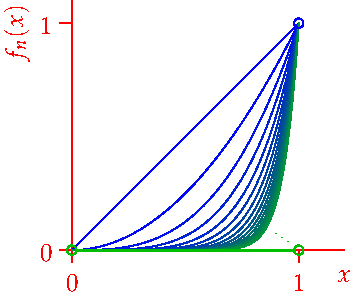
\includegraphics{seqex2}
\end{minipage}
\end{example*}

The example is nice in that a sequence of continuous functions converges pointwise to a continuous function. Unfortunately, this desirable situation is not universal.

\begin{example*}[lower separated=false, sidebyside, sidebyside align=top seam, sidebyside gap=0pt, righthand width=0.4\linewidth]{\ref{ex:seqfn}, mk.\ III}{}
Extend the domain to include $x=1$; define
\[g_n:(0,1]\to\R: x\mapsto x^n\]
Each $g_n$ is a continuous function, however its \textcolor{Green}{pointwise limit}
\[g(x)=\begin{cases}
0&\text{if }x<1\\
1&\text{if }x=1
\end{cases}\]
has a \emph{jump discontinuity} at $x=1$.
\tcblower
\flushright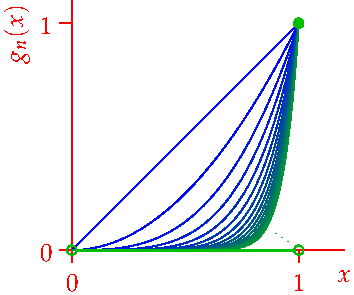
\includegraphics{seqex3}
\end{example*}



% 
% This failure of the pointwise limit to be continuous is not merely a problem that can arise at endponts of an interval: for instance, extending the domain further so that
% \[h_n:[0,2]\to\R:x\mapsto\begin{cases}
% x^n&\text{if }x\le 1\\
% 1&\text{if }x>1
% \end{cases}\]
% we see that each $h_n$ is continuous, and yet its pointwise limit
% \[h:[0,2]\to\R:x\mapsto\begin{cases}
% 0&\text{if }x<1\\
% 1&\text{if }x\ge 1
% \end{cases}\]
% is again discontinuous at $x=1$.\goodbreak




With the goal of having convergence of functions preserve continuity, we make a tighter definition.


\begin{defn}[lower separated=false, sidebyside, sidebyside align=top seam, sidebyside gap=0pt, righthand width=0.32\linewidth]{}{unifconv}
$(f_n)$ \emph{converges uniformly} to $f$ on $U$ if either
\begin{enumerate}
  \item $\displaystyle \sup\limits_{x\in U}\nm{f_n(x)-f(x)}\xrightarrow[n\to\infty]{}0$,\quad or,
  \item $\forall \epsilon>0,\ \textcolor{orange}{\exists N}$ such that $\textcolor{purple}{\forall x}\in U$, $n>N\implies \nm{f_n(x)-f(x)}<\epsilon$
\end{enumerate}
A common notation is $f_n\rightrightarrows f$, though we won't use it.
\tcblower
\flushright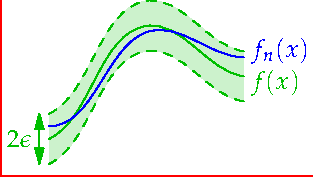
\includegraphics{unifconv1}
\end{defn}

Whenever $n>N$, the graph of $\textcolor{blue}{f_n(x)}$ must lie between those of $\textcolor{Green}{f(x)\pm\epsilon}$.\smallbreak

We'll show that statements 1 and 2 are equivalent momentarily. For the present, compare with the corresponding statements for pointwise convergence:
\begin{itemize}
  \item As with \emph{continuity} versus \emph{uniform continuity,} the distinction comes in the \emph{order of the quantifiers}: in uniform convergence, $x$ is quantified \emph{after} $N$ and so \emph{the same $N$ works for all $x$.}
  \item Uniform convergence implies pointwise convergence.
\end{itemize}

For the last time, we revisit our main example.
\begin{example*}{\ref{ex:seqfn}, mk.\ IV}{}
If $f_n:(0,1)\to\R:x\mapsto x^n$ and $f$ are defined as before, then the pointwise convergence $f_n\to f$ is \emph{non-uniform.} We show this using both criteria.\smallbreak
\begin{minipage}{0.68\linewidth}\vspace{0pt}
\begin{enumerate}
  \item For \emph{every} $n$,
  \[\sup_{x\in(0,1)}\nm{f_n(x)-f(x)} =\sup\{x^n:0<x<1\}=1 \nrightarrow 0\]
  \item Suppose the convergence were uniform and let %\footnotemark
   $\epsilon=\frac 12$. Then 
  \[\exists N\in\N\text{ such that }\forall x\in (0,1),\ n>N\implies x^n<\frac 12\]
  Since $N\in\N$, a simple choice results in a contradiction;
  \[x=\left(\frac 12\right)^{\frac 1{N+1}}\in(0,1)\implies x^{N+1}=\frac 12\]
\end{enumerate} 
  \end{minipage}
  \begin{minipage}{0.31\linewidth}\vspace{0pt}
	\flushright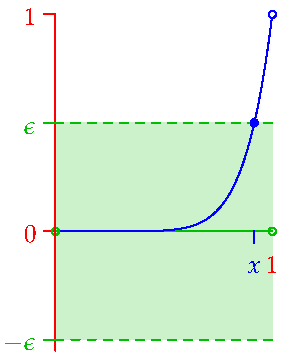
\includegraphics{unifconv2}
  \end{minipage}
\end{example*}

%\footnotetext{We choose $\epsilon=\frac 12$ since this is less than the size of the `jump' in $f_n$ as $n\to\infty$: compare with $g_n$ in the same example.}

\goodbreak


\begin{thm}{}{}
The criteria for uniform convergence in Definition \ref{defn:unifconv} are equivalent.
\end{thm}

\begin{proof}
($1\Rightarrow 2$)\quad This follows from the fact that
\[\forall x\in U,\ \nm{f_n(x)-f(x)}\le\sup_{x\in U}\nm{f_n(x)-f(x)}\]
($2\Rightarrow 1$)\quad Suppose $\epsilon>0$ is given. Then
\[\exists N\in\R\text{ such that }\forall x\in U,\ n>N\implies\nm{f_n(x)-f(x)}<\frac\epsilon 2\]
But then
\[n>N\implies\sup_{x\in U}\nm{f_n(x)-f(x)}\le\frac\epsilon 2<\epsilon\tag*{\qedhere}\]
\end{proof}



Somewhat amazingly, the subtle change of definition results in the preservation of continuity.

\begin{thm}{}{unifcontlimit}
Suppose that $(f_n)$ is a sequence of continuous functions. If $f_n\to f$ uniformly, then $f$ is continuous.
\end{thm}

\begin{proof}
We demonstrate the continuity of $f$ at $a\in U$. Let $\epsilon>0$ be given.
\begin{itemize}
  \item Since $f_n\to f$ uniformly,
	\[\exists N\text{ such that }\forall x\in U,\ n>N\implies\nm{f(x)-f_n(x)}<\frac\epsilon 3\]
	\item Choose any $n>N$. Since $f_n$ is continuous at $a$,
	\[\exists \delta>0\text{ such that }\nm{x-a}<\delta\implies\nm{f_n(x)-f_n(a)} <\frac\epsilon 3\tag{$\dag$}\]
\end{itemize}
Simply put these together with the triangle inequality to see that
\begin{align*}
\nm{x-a}<\delta\implies\nm{f(x)-f(a)}&\le\nm{f(x)-f_n(x)}+\nm{f_n(x)-f_n(a)}+\nm{f_n(a)-f(a)}\\
&<\frac\epsilon 3+\frac\epsilon 3+\frac\epsilon 3=\epsilon \tag*{\qedhere}
\end{align*}
\end{proof}

We need not have fixed $a$ at the start of the proof. Rewriting $(\dag)$ to become
\[\exists\delta>0\text{ such that }\forall x,a\in U,\ \nm{x-a}<\delta\implies\nm{f_n(x)-f_n(a)}<\frac\epsilon 3\]
proves a related result.

\begin{cor}{}{}
If $f_n\to f$ uniformly where each $f_n$ is \emph{uniformly} continuous, then $f$ is uniformly continuous.
\end{cor}

\vfil\goodbreak


\begin{examples}{}{}
\exstart Let $f_n(x)=x+\frac 1nx^2$. This is continuous on $\R$ for all $x$, and converges pointwise to the continuous function $f:x\mapsto x$.
\begin{enumerate}\setcounter{enumi}{1}
  \item[]\begin{enumerate}
    \item On any bounded interval $[-M,M]$ the convergence $f_n\to f$ is uniform,
    \[\sup_{x\in[-M,M]}\nm{f_n(x)-f(x)}=\sup\left\{\frac 1nx^2:x\in[-M,M]\right\}=\frac{M^2}n \xrightarrow[n\to\infty]{}0\]
    \item On any unbounded interval, $\R$ say, the convergence is non-uniform,
    \[\sup_{x\in\R}\nm{f_n(x)-f(x)}=\sup\left\{\frac 1nx^2:x\in\R\right\}=\infty %\nxrightarrow{n\to\infty} 0
    \]
  \end{enumerate}
  
  \begin{minipage}[t]{0.53\linewidth}\vspace{0pt}
  \item Consider $f_n(x)=\frac 1{1+x^n}$; this is continuous on $(-1,\infty)$ and converges pointwise to
  \[\textcolor{Green}{f(x)=\begin{cases}
  0&\text{if }x>1\\
  \frac 12&\text{if }x=1\\
  1&\text{if }-1<x<1
  \end{cases}}\]
  We consider the convergence $f_n\to f$ on several intervals.
  \end{minipage}\begin{minipage}[t]{0.46\linewidth}\vspace{0pt}
  \flushright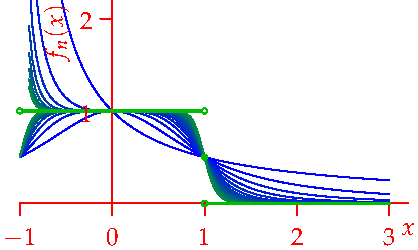
\includegraphics{seqex4}
  \end{minipage}

  \begin{enumerate}
    \item On $[2,\infty)$, the pointwise limit is continuous. Moreover, $f_n(x)$ is decreasing, whence
    \[\sup_{x\in[2,\infty)}\nm{f_n(x)-0}=\frac 1{1+2^n}\xrightarrow[n\to\infty]{} 0\]
    and the convergence is uniform. Alternatively; if $\epsilon\in (0,1)$, let $N=\log_2(\epsilon^{-1}-1)$, then
    \[\forall x\ge 2,\ n>N\implies \nm{f_n(x)-0}=\frac 1{1+x^n}\le \frac 1{1+2^n}<\frac 1{1+2^N}=\epsilon\]
    The same argument shows that $f_n\to f$ uniformly on any interval $[a,\infty)$ where $a>1$.
    \item On $[1,\infty)$ the convergence is not uniform, since the pointwise limit is discontinuous,
		\[f(x)=\begin{cases}
    	0&\text{if }x>1\\
    	\frac 12&\text{if }x=1
    	\end{cases}\]
   	\item The convergence is not even uniform on the open interval $(1,\infty)$,
    \[\sup_{x\in[1,\infty)}\nm{f_n(x)-f(x)}=\sup\left\{\frac 1{1+x^n}:x>1 \right\}=\frac 12\nxrightarrow{n\to\infty} 0\]
    \item Similarly, for any $a\in(0,1)$, the convergence $f_n\to f$ is uniform on $[0,a]$, this time to the (continuous) constant function $f(x)=1$,
    \[\sup_{x\in[0,a]}\nm{f_n(x)-1}=\nm{1-\frac 1{1+a^n}}=\frac{a^n}{1+a^n}\xrightarrow[n\to\infty]{} 0\]
    \item Finally, on $(-1,1)$ the convergence is not uniform,
    \[\sup_{x\in[0,1)}\nm{f_n(x)-f(x)}=\sup\left\{\frac{x^n}{1+x^n}:x\in[0,1) \right\}=\frac 12\nxrightarrow{n\to\infty} 0\]
  \end{enumerate}
\end{enumerate}
\end{examples}

\begin{exercises}
	\emph{Key concepts:\quad ?????}
	
	\begin{enumerate}
		\item\label{exs:uniform1} For each sequence of functions defined on $[0,\infty)$:
		\begin{enumerate}
	    \item[(i)] Find the pointwise limit $f(x)$ as $n\to\infty$.
	    \item[(ii)] Determine whether $f_n\to f$ uniformly on $[0,1]$.
	    \item[(iii)] Determine whether $f_n\to f$ uniformly on $[1,\infty)$.
	  \end{enumerate}\vspace{-12pt}
	  \begin{align*}
	  \text{(a)}&\quad f_n(x)=\frac xn\qquad 
	  &\text{(b)}&\quad f_n(x)=\frac{x^n}{1+x^n}\qquad
	  &\text{(c)}&\quad f_n(x)=\frac{x^n}{n+x^n}\\[4pt]
	  \text{(d)}&\quad f_n(x)=\frac x{1+nx^2}\qquad
	  &\text{(e)}&\quad f_n(x)=\frac{nx}{1+nx^2}
	  \end{align*}
	 	
	 	\item Let $f_n(x)=\left(x-\frac 1n\right)^2$. If $f(x)=x^2$, we clearly have $f_n\to f$ pointwise on any domain.
	 	\begin{enumerate}
	 	  \item Prove that the convergence is uniform on $[-1,1]$.
	 	  \item Prove that the convergence is non-uniform on $\R$.
	 	\end{enumerate}
	  
	  \item For each sequence, find the pointwise limit and decide if the convergence is uniform.
	  \begin{enumerate}
	    \item $f_n(x)=\frac{1+2\cos^2(nx)}{\sqrt n}$ for $x\in\R$.
	    \item $f_n(x)=\cos^n(x)$ on $[-\pi/2,\pi/2]$.
	  \end{enumerate}
	 	
	
		\item\label{ex:classicnonuniform} For each $n\in\N$, consider the continuous function
		\[f_n:[0,1]\to\R:x\mapsto nx^n(1-x)\]
		\begin{enumerate}
		  \item Given $0\le x<1$, let $a\in(x,1)$. Explain why
		   %Since $\lim\limits_{n\to\infty}\frac{f_{n+1}(x)}{f_n(x)}=x<a$,
		   $\exists N$ such that
		  \[n>N\implies \nm{f_{n+1}(x)}\le a\nm{f_n(x)}\]
		  Hence conclude that the pointwise limit of $(f_n)$ is the zero function.
	% 	  \item For any $n,N\in\N$ prove that $n>N\implies \frac{n+1}n<\frac{N+1}N=1+\frac 1N$
	% 	  \item Suppose $x\in(0,1)$ is given and let $N\in\N$ satisfy $x<1-\frac 1N$. Prove that
	% 	  \[n>N\implies \frac{f_n(x)}{f_N(x)} =\frac{n}{n-1}\cdots\frac{N+1}Nx^{n-N}<\left(1-\frac 1{N^2}\right)^{n-N}\]
	% 	  Hence conclude that $f_n$ converges pointwise to the zero function.
		  \item Use elementary calculus $(f'_n(x)=0\iff\ldots)$ to prove that the maximum value of $f_n$ is located at \textcolor{Green}{$x_n=\frac n{1+n}$}. Hence compute
			\[\sup_{x\in[0,1]}\nm{f_n(x)-f(x)}\]
			and use it to show that the convergence $f_n\to 0$ is non-uniform.
		\end{enumerate}
		
		\emph{This shows that the converse to Theorem \ref{thm:unifcontlimit} is false, even on a bounded interval: the continuous sequence $(f_n)$ converges \emph{non-uniformly} to a continuous function. Sketches of several $f_n$ are below.} 
		\begin{center}
		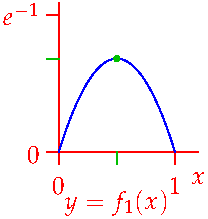
\includegraphics{seqex5}\hfill
		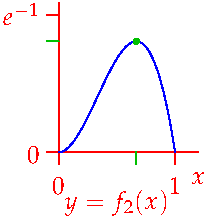
\includegraphics{seqex6}\hfill 
		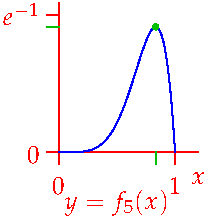
\includegraphics{seqex7}\hfill
		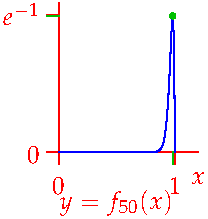
\includegraphics{seqex8}
		\end{center}
	
		\item Explain where the proof of Theorem \ref{thm:unifcontlimit} fails if $f_n\to f$ \emph{non-uniformly.}
	\end{enumerate}
\end{exercises}
\goodbreak


\subsection{More on Uniform Convergence}\label{sec:unifconvmore}

While we haven't yet developed calculus, our familiarity with basic differentiation and integration makes it natural to pause to consider the interaction of these operations with sequences of functions.\smallbreak

We also consider a Cauchy-criterion for uniform convergence, which leads to the useful Weierstraß\ $M$-test.

\begin{example}{}{diffinteasy}
Recall that $f_n(x)=x^n$ converges uniformly to $f(x)=0$ on any interval $[0,a]$ where $a<1$. We easily check that
  \[\int_0^af_n(x)\,\dx=\frac 1{n+1}a^{n+1}\xrightarrow[n\to\infty]{} 0 =\int_0^af(x)\,\dx\]
  In fact the sequence of derivatives converge here also
  \[\diff xf_n(x)=nx^{n-1} \xrightarrow[n\to\infty]{} 0 =f'(x)\]
\end{example}

It is perhaps surprising that integration interacts more nicely with uniform limits than does differentiation. We therefore consider integration first.

\begin{thm}{}{unifintegral}
Let $f_n\to f$ uniformly on $[a,b]$ where the functions $f_n$ are integrable. Then $f$ is integrable on $[a,b]$ and
\[\lim_{n\to\infty}\int_a^bf_n(x)\dx=\int_a^bf(x)\dx\]
\end{thm}

\begin{proof}
Given $\epsilon>0$, note that $\int_a^b\frac\epsilon{2(b-a)}\,\dx=\frac\epsilon 2$. Since $f_n\to f$ uniformly, $\exists N$ such that\footnotemark
\begin{align*}
\forall x\in [a,b],\ n>N&\implies \nm{f_n(x)-f(x)}<\frac\epsilon{2(b-a)}\\
&\implies f_n(x)-\frac\epsilon{2(b-a)}<f(x)< f_n(x)+\frac\epsilon{2(b-a)}\\
&\implies \int_a^b f_n(x)\,\dx-\frac\epsilon 2\le \int_a^bf(x)\,\dx\le \int_a^b f_n(x)\,\dx+\frac\epsilon 2\\
&\implies \nm{\int_a^bf_n(x)\,\dx-\int_a^bf(x)\,\dx}\le \frac\epsilon 2<\epsilon\tag*{\qedhere}
\end{align*}
\end{proof}

\footnotetext{This assumes $f$ is already integrable. Once we've properly defined (Riemann) integrability at the end of the course, we can insert the following
\[\int_a^b f_n(x)\,\dx-\frac\epsilon 2\le L(f)\le U(f)\le \int_a^b f_n(x)\,\dx+\frac\epsilon 2
\implies 0\le U(f)-L(f)\le \epsilon\implies U(f)=L(f)\]
where $U(f)$ and $L(f)$ are the upper and lower Darboux integrals of $f$; their equality shows that $f$ is integrable on $[a,b]$.}

The appearance of uniform convergence in the proof is subtle. If $N=N(\epsilon)$ were allowed to depend on $x$, then the integral $\int_a^bf_n(x)\,\dx$ would be meaningless: Which $n$ would we consider? Larger than $N(x,\epsilon)$ for \emph{which} $x$? Taking $n$ `larger' than \emph{all} the $N(x,\epsilon)$ might produce the absurdity $n=\infty$!\goodbreak

\begin{examples}{}{intnotconvout}
\exstart Uniform convergence is not required for the integrals to converge as we'd like. For instance, recall that extending the previous example to the domain $[0,1]$ results in non-uniform convergence; however, we still have
	\[\int_0^1f_n(x)\,\dx=\frac 1{n+1}\xrightarrow[n\to\infty]{} 0 =\int_0^1f(x)\,\dx\]
  %Since $f$ is discontinuous, the final integral requires a little care.
  
\begin{enumerate}\setcounter{enumi}{1}
  \item\label{ex:intnotconv} To obtain a sequence of functions $f_n\to f$ for which $\int f_n\nrightarrow\int f$ requires a bit of creativity. Consider the sequence\smallbreak
  \begin{minipage}[t]{0.6\linewidth}\vspace{-15pt}
  \begin{align*}
  f_n&:[-1,1]\to\R :x\mapsto \begin{cases}
  n-n^2x&\text{if }0<x<\frac 1n\\
  0&\text{otherwise}
  \end{cases}
  \end{align*}
  If $0<x<1$, then for large $n\in\N$ we have
  \[x\ge\frac 1n\implies f_n(x)=0\]
  \end{minipage}\begin{minipage}[t]{0.4\linewidth}\vspace{-10pt}
  \flushright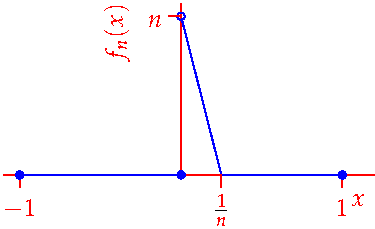
\includegraphics{seqex10}
  \end{minipage}\\[0pt]
  We conclude that $f_n\to 0$ pointwise. Since the area under $f_n$ is a triangle with base $\frac 1n$ and height $n$, the integral is constant and \emph{non-zero};
  \[\int_{-1}^1 f_n(x)\,\dx=\frac 12\neq 0=\int_{-1}^1f(x)\,\dx\]
  It should be obvious why the convergence $f_n\to 0$ is non-uniform; why?
\end{enumerate}
\end{examples}


\boldinline{Derivatives and Uniform Limits}

We've already seen that a uniform limit of differentiable functions \emph{might} be differentiable (Example \ref{ex:diffinteasy}), but this shouldn't be expected in general since even uniform limits of differentiable functions can have corners!

\begin{example}[lower separated=false, sidebyside, sidebyside align=top seam, sidebyside gap=0pt, righthand width=0.4\linewidth]{}{}
For each $n\in\N$, consider the function
\[f_n:[-1,1]\to\R:x\mapsto \begin{cases}
\nm x&\text{if }\nm x\ge\frac 1n\\
\frac n2x^2+\frac 1{2n}&\text{if }\nm x<\frac 1n
\end{cases}\]
\begin{itemize}
  \item $f_n$ converges pointwise to \textcolor{Green}{$f(x)=\nm x$}.
  \item $f_n\to f$ uniformly since\vspace{-5pt}
  \[\sup_{x\in[-1,1]}\nm{f_n(x)-f(x)}=\frac 1{2n}\to 0\]\vspace{-15pt}
 	\item Each $f_n$ is differentiable: $f'_n(x)=\begin{cases}
  1&\text{if }x\ge\frac 1n\\
  nx&\text{if }\nm x<\frac 1n\\
  -1&\text{if }x\le -\frac 1n
  \end{cases}$
  \item The uniform limit $f$ is \emph{not differentiable} at $x=0$.
\end{itemize}
\tcblower
\flushright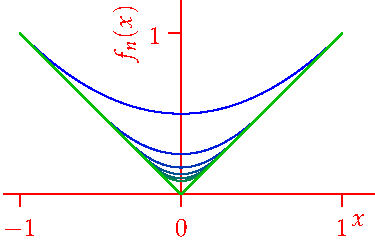
\includegraphics{seqex9}\\
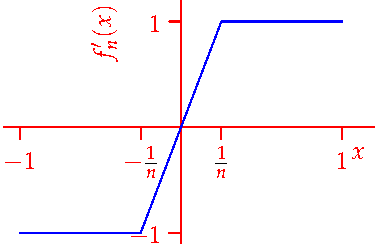
\includegraphics{seqex9-1}
\end{example}\goodbreak


Transferring differentiability to the limit of a sequence of functions is a bit messy.

\begin{thm}{}{unifderiv}
Suppose $(f_n)$ is a sequence and $g$ is a function on $[a,b]$ for which:
\begin{itemize}
  \item $f_n\to f$ pointwise;
  \item Each $f_n$ is differentiable with continuous derivative;\footnotemark
  \item $f_n'\to g$ uniformly.
\end{itemize}
Then $f_n\to f$ uniformly on $[a,b]$ and $f$ is differentiable with derivative $g$.
\end{thm}

\footnotetext{Without the continuity assumption, the fundamental theorem of calculus doesn't apply and the proof requires an alternative approach. One can also weaken the hypotheses: if $f'_n\to g$ uniformly and that $(f_n(x))$ converges for \emph{at least one} $x\in [a,b]$, then there exists $f$ such that $f_n\to f$ is uniform and $f'=g$.}

The issue in the previous example is that the \emph{pointwise limit} of the derived sequence $(f'_n)$ is discontinuous at $x=0$ and therefore $f'_n\to g$ isn't uniform! 

\begin{proof}
For any $x\in [a,b]$, the fundamental theorem of calculus tells us that
\[\int_a^x f'_n(t)\,\dt  = f_n(x)-f_n(a)\]
By Theorem \ref{thm:unifintegral}, the left side converges to $\int_a^x g(t)\,\dt$, while the right converges to $f(x)-f(a)$. Since $f_n'\to g$ uniformly, we see that $g$ is continuous and we can apply the fundamental theorem again: $\int_a^xg(t)\,\dt=f(x)-f(a)$ is differentiable with derivative $g$.\smallbreak
The uniformity of the convergence $f_n\to f$ follows from Exercise \ref{ex:derivunifconvtidy}.
\end{proof}


\subsubsection*{Uniformly Cauchy Sequences and the Weierstraß $M$-Test}

Recall that one may use Cauchy sequences to demonstrate convergence \emph{without knowing the limit in advance.} An analogous discussion is available for sequences of functions.


\begin{defn}{}{}
A sequence of functions $(f_n)$ is \emph{uniformly Cauchy} on $U$ if
\[\forall\epsilon>0,\ \exists N\in\N \text{ such that }\forall x\in U,\ m,n>N\implies\nm{f_n(x)-f_m(x)}<\epsilon\]
\end{defn}

\begin{example}{}{unifcauchy}
Let $f_n(x)=\sum\limits_{k=1}^n\frac 1{k^2}\sin k^2x$ be defined on $\R$. Given $\epsilon>0$, let $N=\frac 1\epsilon$, then\vspace{-10pt}
\begin{align*}
m>n>N\implies \nm{f_m(x)-f_n(x)}&=\nm{\sum_{k=n+1}^m\frac 1{k^2}\sin k^2x} \le\sum_{k=n+1}^m\frac 1{k^2} \le\sum_{k=n+1}^m\frac 1{k(k-1)}\\
&=\sum_{k=n+1}^m\frac 1{k-1}-\frac 1k =\frac 1n-\frac 1m<\frac 1N=\epsilon
\end{align*}
whence $(f_n)$ is uniformly Cauchy.
\end{example}\goodbreak

As with sequences of real numbers, uniformly Cauchy sequences converge; in fact uniformly!

\begin{thm}{}{}
A sequence $(f_n)$ is uniformly Cauchy on $U$ if and only if it converges uniformly to some $f:U\to\R$.
\end{thm}

\begin{proof}
($\Rightarrow$)\quad Let $(f_n)$ be uniformly Cauchy on $U$. For each $x\in U$, the sequence $(f_n(x))\subseteq\R$ is Cauchy and thus convergent. Define $f:U\to\R$ via
\[f(x):=\lim\limits_{n\to\infty}f_n(x)\]
We claim that $f_n\to f$ uniformly. Let $\epsilon>0$ be given, then 
\begin{align*}
\exists N\in\N\text{ such that }m>n>N&\implies \nm{f_n(x)-f_m(x)}<\frac\epsilon 2\\
&\implies f_n(x)-\frac\epsilon 2<f_m(x)<f_n(x)+\frac\epsilon 2\\
&\implies f_n(x)-\frac\epsilon 2\le f(x)\le f_n(x)+\frac\epsilon 2 \tag{take limits as $m\to\infty$}\\
&\implies \nm{f_n(x)-f(x)}\le\frac\epsilon 2<\epsilon
\end{align*}
($\Leftarrow$)\quad This is Exercise \ref{ex:cauchyexproof}.
\end{proof}


\begin{example*}{\ref{ex:unifcauchy}, mk.\ II}{}
Since $(f_n)$ is uniformly Cauchy on $\R$, it converges uniformly to some $f:\R\to\R$. It seems reasonable to write
\[f(x)=\sum\limits_{n=1}^\infty\frac 1{n^2}\sin n^2x\]
The graph of this function looks somewhat bizarre:
\begin{center}
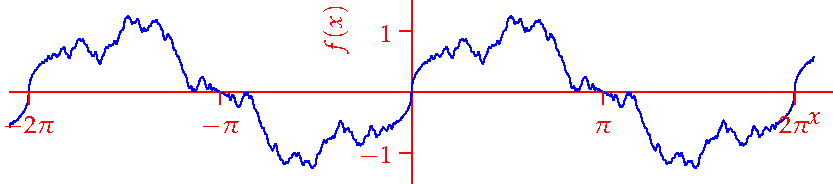
\includegraphics{unifcauchy}
\end{center}
Since each $f_n$ is (uniformly) continuous, Theorem \ref{thm:unifcontlimit} says that $f$ is also (uniformly) continuous. By Theorem \ref{thm:unifintegral}, $f(x)$ is integrable, indeed
\[\int_a^bf(x)\,\dx=\lim_{n\to\infty}\sum_{k=1}^n -k^{-4}\cos k^2x\big|_a^b =\sum_{n=1}^\infty \frac 1{n^4}(\cos n^2a-\cos n^2b)\]
which converges (comparison test) for all $a,b$. By contrast, the derived sequence 
\[f'_n(x)=\sum\limits_{k=1}^n \cos k^2x\]
does not converge for \emph{any} $x$ since $\cos n^2x\nxrightarrow{k\to\infty} 0$. We should thus expect (though we offer no proof) that $f$ is nowhere differentiable.
\end{example*}



The example generalizes. Suppose $(g_k)$ is a sequence of functions on $U$ and define the \emph{series} $\sum g_k(x)$ as the pointwise limit of the sequence $(f_n)$ of partial sums
\[\sum_{k=k_0}^\infty g_k(x):=\lim\limits_{n\to\infty}f_n(x)\quad\text{where}\quad f_n(x)=\sum_{k=k_0}^ng_k(x)\]
whenever the limit exists. The series is said to converge uniformly whenever $(f_n)$ does so. Theorems \ref{thm:unifcontlimit}, \ref{thm:unifintegral} and \ref{thm:unifderiv} immediately translate.

\begin{cor}{}{unifseries}
Let $\sum g_k$ be a series of functions converging uniformly on $U$. Then:
\begin{enumerate}
  \item If each $g_k$ is (uniformly) continuous then $\sum g_k$ is (uniformly) continuous.
  \item If each $g_k$ is integrable, then $\int\sum g_k(x)\,\dx=\sum\int g_k(x)\,\dx$.
  \item If each $g_k$ is continuously differentiable, and the sequence of derived partial sums $f'_n$ converges uniformly, then $\sum g_k$ is differentiable and $\diff x\sum g_k(x)=\sum g'_k(x)$.
\end{enumerate}
\end{cor}\goodbreak

As an application of the uniform Cauchy criterion, we obtain an easy test for uniform convergence.

\begin{thm}{Weierstraß $M$-test}{}
Suppose $(g_k)$ is a sequence of functions on $U$. Moreover assume:
\begin{enumerate}
  \item $(M_k)$ is a non-negative sequence such that $\sum M_k$ converges.
  \item Each $g_k$ is bounded by $M_k$; that is $\nm{g_k(x)}\le M_k$.
\end{enumerate}
Then $\sum g_k(x)$ converges uniformly on $U$.
\end{thm}

\begin{proof}
Let $f_n(x)=\sum\limits_{k=k_0}^ng_k(x)$ define the sequence of partial sums. Since $\sum M_k$ converges, its sequence of partial sums is Cauchy (the \emph{Cauchy criterion} for infinite series); given $\epsilon>0$,
\[\exists N\text{ such that }m>n>N\implies \sum_{k=n+1}^m M_k<\epsilon\]
However, by assumption,
\[m>n>N\implies \nm{f_m(x)-f_n(x)}=\nm{\sum_{k=n+1}^mg_k(x)} \le \sum_{k=n+1}^m\nm{g_k(x)} \le\sum_{k=n+1}^mM_k<\epsilon\tag*{\qedhere}\]
The sequence of partial sums is uniformly Cauchy and thus uniformly convergent.
\end{proof}

\begin{example}{}{mtestex}
Given the series $\sum\limits_{n=1}^\infty\frac{1+\cos^2(nx)}{n^2}\sin(nx)$, we clearly have
\[\nm{\frac{1+\cos^2(nx)}{n^2}\sin(nx)}\le\frac 2{n^2}\text{ for all }x\in\R\]
Since $\sum\frac 2{n^2}$ converges, the $M$-test shows that the original series converges uniformly on $\R$.
\end{example}

\goodbreak

\begin{exercises}
	\emph{Key concepts:\quad ?????}

	\begin{enumerate}
		\item For each $n\in\N$, let $f_n(x)=nx^n$ when $x\in[0,1)$ and $f_n(1)=0$.
		\begin{enumerate}
	    \item Prove that $f_n\to 0$ pointwise on $[0,1]$.\\
	    (\emph{Hint: recall Exercise \hyperref[ex:classicnonuniform]{\ref*{sec:uniformconv}.\ref*{ex:classicnonuniform}} if you're not sure how to prove this})
	    \item By considering the integrals $\int_0^1f_n(x)\,\dx$ show that $f_n\to 0$ is not uniform.
	  \end{enumerate}
	  
	  \item\label{ex:cauchyexproof} Prove that if $f_n\to f$ uniformly, then the sequence $(f_n)$ is uniformly Cauchy.
	  
	  \item\begin{enumerate}
	    \item Suppose $(f_n)$ is a sequence of bounded functions on $U$ and suppose that $f_n\to f$ converges uniformly on $U$. Prove that $f$ is bounded on $U$.
	    \item Give an example of a sequence of bounded functions $(f_n)$ converging pointwise to $f$ on $[0,\infty)$, but for which $f$ is \emph{unbounded.}
	  \end{enumerate}
	  
	  \item The sequence defined by $f_n(x)=\frac{nx}{1+nx^2}$ (Exercise \hyperref[exs:uniform1]{\ref*{sec:uniformconv}.1}) converges uniformly on any closed interval $[a,b]$ where $0<a<b$.
	  \begin{enumerate}
	    \item Check explicitly that $\int_a^b f_n(x)\,\dx\to \int_a^bf(x)\,\dx$, where $f=\lim f_n$.
	    \item Is the same thing true for derivatives?
	  \end{enumerate}
	  
	 	\item Let $f_n(x)=n^{-1}\sin n^2x$ be defined on $\R$.
	 	\begin{enumerate}
	 	  \item Prove that $f_n$ converges uniformly on $\R$.
	 	  \item Check that $\int_0^x f_n(t)\,\dt$ converges for any $x\in\R$.
	 	  \item Does the derived sequence $(f_n')$ converge? Explain.
	 	\end{enumerate}
	  
	%   \item As another example, we've already seen (page \pageref{ex:classicnonuniform}) that the pointwise convergence $f_n\to 0$ where $f_n(x)=nx^n(1-x)$ is not uniform. However the integrals still converge;
	% 	\[\int_0^1f_n(x)\,\dx=\frac n{n+1}-\frac n{n+2}\xrightarrow[n\to\infty]{} 0=\int_0^1f(x)\,\dx\]
		
	
		
		\item Use the $M$-test to prove that $\smash[b]{\sum\limits_{n=1}^\infty\frac{x^n}{n^2}}$ defines a continuous function on $[-1,1]$.
	  
	  \item Prove that $\sum\limits_{n=1}^\infty\frac{x^n\sin x}{(n+1)^32^n}$ converges uniformly to a continuous function on the interval $[-2,2]$.
	
	 \item Prove that if $\sum g_k$ converges uniformly on a set $U$ and if $h$ is a bounded function on $U$, then $\sum hg_k$ converges uniformly on $U$.\\
	 (\emph{Warning: you cannot simply write $\sum hg_k=h\sum g_k$})
	
	% 	\item $f_n(x)=n^{-1}e^{-nx}$ on $[0,\infty)$ converges uniformly to $f(x)=0$ since $\nm{f_n(x)}\le \frac 1n$. However
	% \[f'_n(x)=-e^{-nx}\]
	% only converges to $f'(x)=0$ when $x>0$, and only uniformly so on intervals $[a,\infty)$ where $a>0$.\goodbreak	
	
		\item Consider Example \hyperref[ex:intnotconv]{\ref*{ex:intnotconvout}.\ref*{ex:intnotconv}}.
		\begin{enumerate}
		  \item Check explicitly that the convergence isn't uniform by computing $\sup\limits_{x\in[-1,1]}\nm{f_n(x)-f(x)}$
		  \item Prove that $f_n\to 0$ pointwise on $(0,1]$ using the $\epsilon$--$N$ definition of convergence: that is, given $\epsilon>0$ and $x\in(0,1]$, find an explicit $N(x,\epsilon)$ such that
	  	\[n>N\implies \nm{f(x)}<\epsilon\]
	  	What happens to your choice of $N(x,\epsilon)$ as $x\to 0^+$?
		\end{enumerate}
		
		\item\label{ex:derivunifconvtidy} Suppose $(f_n')$ converges uniformly on $[a,b]$ and that each $f_n'$ is continuous.
		\begin{enumerate}
		  \item Use the fact that $(f_n')$ is uniformly Cauchy to prove that $(f_n)$ is uniformly Cauchy and thus converges uniformly to some function $f$.\\
			(\emph{Hint: $\nm{f_n(x)-f_m(x)}=\nm{\int_a^xf_n'(t)-f_m'(t)\,\dt}\ldots$})
			\item Explain why we need not have assumed the existence of $f$ in Theorem \ref{thm:unifderiv}.
		\end{enumerate}
	\end{enumerate}
\end{exercises}


\goodbreak


\subsection{Differentiation and Integration of Power Series}\label{sec:diffintpower}

In this section we specialize our recent results to power series. While everything will be stated for series centered at $x=0$, all are easily translated to arbitrary centers.

\begin{thm}{}{unifpowerseries}
Let $\sum a_nx^n$ be a power series with radius of convergence $R>0$ and let $T\in(0,R)$. Then:
\begin{enumerate}
  \item The series converges uniformly on $[-T,T]$.
  \item The series is uniformly continuous on $[-T,T]$ and continuous on $(-R,R)$.
\end{enumerate} 
\end{thm}

\vfil

\begin{proof}
This is an easy application of the $M$-test. For each $k$, define $M_k=\nm{a_k}T^k$,
\[T<R\implies \sum a_nT^n\text{ converges absolutely }\implies \sum M_k\text{ converges}\]
By the $M$-test and Corollary \ref{cor:unifseries}, the power series converges uniformly on $[-T,T]$ to a uniformly continuous function.\medbreak

Finally, every $x\in(-R,R)$ lies in some such interval (take $T=\nm x$), whence the power series is continuous on $(-R,R)$.
\end{proof}

%\vfil

\begin{example}{}{geometricps}
On its interval of convergence $(-1,1)$, the geometric series \smash[b]{$\sum\limits_{n=0}^\infty x^n$} converges pointwise to $\frac 1{1-x}$; convergence is uniform on any interval $[-T,T]\subseteq(-1,1)$.\smallbreak
We needn't use the Theorem for this is simple to verify directly: writing $f,f_n$ for the series and its partial sums,
\begin{gather*}
\nm{f_n(x)-f(x)}=\nm{\frac{1-x^{n+1}}{1-x}-\frac 1{1-x}}=\nm{\frac{x^{n+1}}{1-x}}\\
\implies \sup_{x\in [-T,T]}\nm{f_n(x)-f(x)}=\frac{T^{n+1}}{1-T} \xrightarrow[n\to\infty]{} 0
\end{gather*}
\smallbreak
By contrast, the convergence is non-uniform on $(-1,1)$;
\[\sup_{x\in(-1,1)}\nm{f_n(x)-f(x)}=\infty\]
% The convergence is therefore non-uniform on the interval $(-1,1)$.
\end{example}

\vfil

\begin{thm}{}{psintdiff}
Suppose $\sum\limits_{n=0}^\infty a_nx^n$ has radius of convergence $R>0$. Then the series is integrable and differentiable term-by-term on the interval $(-R,R)$. Indeed for any $x\in(-R,R)$,
\[\diff x\sum\limits_{n=0}^\infty a_nx^n=\sum\limits_{n=1}^\infty na_nx^{n-1}\quad\text{and}\quad\int_0^x\sum\limits_{n=0}^\infty a_nt^n\,\dt=\sum\limits_{n=0}^\infty \frac{a_n}{n+1}x^{n+1}\]
where both series also have radius of convergence $R$.
\end{thm}\goodbreak

\begin{proof}
Let $f(x)=\sum a_nx^n$ have radius of convergence $R$, and observe that
\[\limsup\nm{na_n}^{1/n}=\lim n^{1/n}\limsup\nm{a_n}^{1/n}=\frac 1R\]
whence $\sum na_nx^n$ also has radius of convergence $R$. At any given non-zero $x\in(-R,R)$, we may write
\[\textcolor{blue}{\sum\limits_{n=1}^\infty na_nx^{n-1}}=x^{-1}\sum\limits_{n=1}^\infty na_nx^{n}\]
to see that the \textcolor{blue}{derived series} also has radius of convergence $R$. On any interval $[-T,T]\subseteq (-R,R)$, the derived series converges uniformly (Theorem \ref{thm:unifpowerseries}). Since each $a_nx^n$ is continuously differentiable, Corollary \ref{cor:unifseries} says that $f$ is differentiable on $[-T,T]$ and that
\[f'(x)=\sum\limits_{n=0}^\infty\diff xa_nx^n= \sum\limits_{n=1}^\infty na_nx^{n-1}\]
Since any $x\in(-R,R)$ lies in some such interval $[-T,T]$, we are done.\medbreak
The corresponding result for integrals is Exercise \ref{ex:psintegralproof}.
\end{proof}

We postpone the canonical examples until after the next result.


\boldsubsubsection{Continuity at Endpoints?}

There is one small hole in our analysis. If a series has radius of convergence $R$ we know that it converges and is continuous on $(-R,R)$. But what if it additionally converges at $x=\pm R$? Is the series continuous at the endpoints? The answer is an unequivocal yes, though this small benefit requires a lot of work!

\begin{thm}{Abel's Theorem}{}
Power series are continuous on their full interval of convergence.
\end{thm}



\def\exexabel{1}

\begin{examples}{}{abel}
\exstart\phantomsection\label{ex:abel1} Apply our results to the geometric series;
\[\frac 1{(1-x)^2}=\diff x\frac 1{1-x}=\sum_{n=1}^\infty nx^{n-1}=\sum_{n=0}^\infty (n+1)x^n=1+2x+3x^2+4x^3+\cdots\]
  \[\ln(1-x)=-\int_0^x\frac 1{1-t}\,\dt= -\sum_{n=0}^\infty\frac 1{n+1}x^{n+1}
  =-\sum_{n=1}^\infty \frac 1nx^n=-\left(x+\frac 12x^2+\frac 13x^3+\cdots\right)\]
  with both series valid on $(-1,1)$. In fact the first series has the same interval of convergence, while the second is $[-1,1)$. By Abel's Theorem and the fact that logarithms are continuous, we have equality at $x=-1$ and the famous identity
  \[\ln 2=\sum_{n=1}^\infty \frac{(-1)^{n+1}}{n}=1-\frac 12+\frac 13-\frac 14+\cdots\]
	%While the formula is nice, recalling the alternating series test, one sees that the convergence is very slow $\nm{\ln 2-\sum_{k=1}^n\frac{(-1)^{k+1}}{k}}<\frac 1n$.
	This example shows that while the integrated and differentiated series have the same radius of convergence as the original, convergence at the endpoints need not be the same in all cases.
	
\begin{enumerate}\setcounter{enumi}{1}  
	\item Substitute $x\mapsto -x^2$ in the geometric series and integrate term-by-term: if $\nm x<1$, then
	\[\frac 1{1+x^2}=\sum_{n=0}^\infty(-1)^nx^{2n} \implies  \arctan x=\sum_{n=0}^\infty\frac{(-1)^n}{2n+1}x^{2n+1}\]
	In fact the arctangent series also converges at $x=\pm 1$; Abel's Theorem says it is continuous on $[-1,1]$. Since arctangent is continuous (on $\R$!) we recover another famous identity
	\[\frac\pi 4=\arctan 1=\sum_{n=0}^\infty\frac{(-1)^n}{2n+1}=1-\frac 13+\frac 15-\frac 17+\cdots\]
	As with the identity for $\ln 2$, this is a very slowly converging alternating series and therefore doesn't provide an efficient method for approximating $\pi$.
  
  \item The series $\displaystyle f(x)=\sum_{n=0}^\infty \frac{(-1)^n}{(2n)!}x^{2n}$ has radius of convergence $\infty$. Differentiate to obtain
	\[f'(x)=\sum_{n=1}^\infty \frac{(-1)^nx^{2n-1}}{(2n-1)!}=\sum_{n=0}^\infty \frac{(-1)^{n+1}}{(2n+1)!}x^{2n+1}\]
	This series is also valid for all $x\in\R$. Differentiating again,
	\[f''(x)=\sum_{n=0}^\infty \frac{(-1)^{n+1}}{(2n)!}x^{2n}=-\sum_{n=0}^\infty \frac{(-1)^n}{(2n)!}x^{2n}=-f(x)\]
	Recalling that $f(x)=\cos x$ is the unique solution to the initial value problem
	\[\begin{cases}
	f''(x)=-f(x)\\
	f(0)=1,\ f'(0)=0
	\end{cases}\]
	We conclude that, $\forall x\in\R$,
	\[\cos x=\sum_{n=0}^\infty \frac{(-1)^n}{(2n)!}x^{2n} \qquad \sin x=-f'(x)=\sum_{n=0}^\infty \frac{(-1)^n}{(2n+1)!}x^{2n+1}\]
\end{enumerate}
\end{examples}


These expressions can instead be taken as the \emph{definitions} of sine and cosine. As promised earlier in the course, continuity and differentiability now come for free. One difficulty with this definition is believing that it has anything to do with right-triangles!\\[5pt]
We can similarly define other common transcendental functions using power series: for instance
\[\exp(x)=\sum\limits_{n=0}^\infty \frac 1{n!}x^n %,\qquad \cosh x=\frac{e^x+e^{-x}}2=\sum_{n=0}^\infty \frac{x^{2n}}{(2n)!},\qquad \sinh x=\frac{e^x-e^{-x}}2=\sum_{n=0}^\infty \frac{x^{2n+1}}{(2n+1)!}
\]
Example \hyperref[ex:abel1]{\ref*{ex:abel}.\exexabel} could be taken as a definition of the logarithm on the interval $(0,2]$, 
\[\ln x=\ln(1-(1-x))=-\sum_{n=1}^\infty \frac 1n(1-x)^n =\sum_{n=1}^\infty \frac{(-1)^{n+1}}n(x-1)^n\]
though this is unnecessary since it is more natural to define $\ln$ as the inverse of the exponential.\goodbreak


\subsubsection*{Proof of Abel's Theorem (non-examinable)}

This requires a lot of work, so feel free to omit on a first reading!\bigbreak

First observe that there is nothing to check unless $0<R<\infty$. By the change of variable $x\mapsto \pm\frac xR$, it is enough for us to prove the following:
\[\sum\limits_{n=0}^\infty a_n\text{ convergent and } f(x)=\sum\limits_{n=0}^\infty a_nx^n\text{ on }(-1,1)\implies\lim\limits_{x\to 1^-}f(x)=\sum\limits_{n=0}^\infty a_n\]

\begin{proof}
Let \smash[b]{$s_n=\sum\limits_{k=0}^n a_k$} and write $s=\lim s_n=\sum a_n$. It is an easy exercise to check that
\[\sum_{k=0}^na_kx^k =s_nx^n+(1-x)\sum_{k=0}^{n-1}s_kx^k\]
% , by convention $s_{-1}:=0$ and denote $s=\sum_{n=0}^\infty a_n$. For any $x\in(-1,1)$, observe that
% \begin{align*}
% \sum_{k=0}^na_kx^k =&\sum_{k=0}^n(s_k-s_{k-1})x^k =\sum_{k=0}^ns_kx^k-\sum_{k=0}^{n-1}s_kx^{k+1}=s_nx^n+(1-x)\sum_{k=0}^{n-1}s_kx^k
% \end{align*}
If $\nm x<1$, then (since $s_n\to s$) $\lim s_nx^n=0$, whence we obtain
\[\forall x\in(-1,1),\ f(x)=(1-x)\sum_{n=0}^{\infty}s_nx^n\]
Let $\epsilon\in(0,1)$ be given and fix $x\in(0,1)$. Then
\[\exists N\in\N\text{ such that }n>N\implies \nm{s_n-s}<\frac\epsilon 2 \tag{$\ast$}\]
Use the geometric series formula $\sum\limits_{n=0}^{\infty}x^n=\frac 1{1-x}$ and write $h(x)=(1-x)\nm{\sum\limits_{n=0}^N(s_n-s)x^n}$ to observe
\begin{align*}
\nm{f(x)-s}&=\nm{(1-x)\sum_{n=0}^{\infty}s_nx^n-s} =\nm{(1-x)\sum_{n=0}^{\infty}s_nx^n-s(1-x)\sum_{n=0}^{\infty}x^n}\\
&=\nm{(1-x)\sum_{n=0}^{\infty}(s_n-s)x^n} =(1-x)\nm{\sum_{n=0}^N(s_n-s)x^n+\sum_{n=N+1}^\infty(s_n-s)x^n}\\
&\le (1-x)\nm{\sum_{n=0}^N(s_n-s)x^n}+ (1-x)\nm{\sum_{n=N+1}^\infty(s_n-s)x^n} \tag{$\triangle$-inequality}\\
&<h(x)+ \frac\epsilon 2(1-x)\nm{\sum_{n=N+1}^\infty x^n} \tag{by ($\ast$)}\\
&\le h(x)+ \frac\epsilon 2
\end{align*}
Since $h>0$ is continuous and $h(1)=0$, $\exists \delta>0$ such that $x\in(1-\delta,1)\implies h(x)<\frac\epsilon 2$ (the computation of a suitable $\delta$ is another exercise).\medbreak
We conclude that $\lim\limits_{x\to 1^-}f(x)=s$.
%  and define $S=\max\{\nm{s_n-s}:n\le N\}$ to observe
% \begin{align*}
% \nm{f(x)-s}&=\nm{(1-x)\sum_{n=0}^{\infty}s_nx^n-s} =\nm{(1-x)\sum_{n=0}^{\infty}s_nx^n-s(1-x)\sum_{n=0}^{\infty}x^n}\\
% &=\nm{(1-x)\sum_{n=0}^{\infty}(s_n-s)x^n} =(1-x)\nm{\sum_{n=0}^N(s_n-s)x^n+\sum_{n=N+1}^\infty(s_n-s)x^n}\\
% &\le(1-x)\sum_{n=0}^N S x^n+ (1-x)\nm{\sum_{n=N+1}^\infty(s_n-s)x^n}\\
% &\le S(1-x)\frac{1-x^{N+1}}{1-x}+ \frac\epsilon 2(1-x)\nm{\sum_{n=N+1}^\infty x^n}\\
% &=S(1-x^{N+1})+ \frac\epsilon 2
% \end{align*}
% To finish the proof, let $\delta=1-\left(1-\frac\epsilon{2S}\right)^{\frac 1{N+1}}$ to observe that
% \[x\in(1-\delta,1)\implies x>\left(1-\frac\epsilon{2S}\right)^{\frac 1{N+1}}\implies S(1- x^{N+1})<\frac\epsilon 2\tag*{\qedhere}\]
\end{proof}

\clearpage

\begin{exercises}
	\emph{Key concepts:\quad ?????}

	\begin{enumerate}
	  \item\begin{enumerate}
			\item Prove that $\displaystyle\sum_{n=1}^\infty nx^n=\frac x{(1-x)^2}$ for $\nm x<1$.
	   	\item Evaluate $\displaystyle\sum_{n=1}^\infty\frac n{2^n}$, $\displaystyle\sum_{n=1}^\infty\frac{n}{4^n}$ and $\displaystyle\sum_{n=1}^\infty\frac{(-1)^nn}{4^n}$
	 \end{enumerate}
	 
	 \item\begin{enumerate}
	   \item Starting with a power series centered at $x=0$, evaluate the integral $\displaystyle\int_0^{1/2}\frac 1{1+x^4}\,\dx$ as an infinite series.
	   \item (Harder) Repeat part (a) but for $\displaystyle\int_0^{1}\frac 1{1+x^4}\,\dx$. What extra ingredients do you need? 
	 \end{enumerate}
	 
	 \item The probability that a standard normally distributed random variable $X$ lies in the interval $[a,b]$ is given by the integral
	 \[\pr(a\le X\le b)=\frac 1{\sqrt{2\pi}}\int_a^b\exp\left(-\frac{x^2}2\right)\,\dx\]
	 Find $\pr(-1\le X\le 1)$ as an infinite series.
	
	 \item Define $\displaystyle c(x)=\sum_{n=0}^\infty\frac{x^{2n}}{(2n)!}$ and $\displaystyle s(x)=\sum_{n=0}^\infty\frac{x^{2n+1}}{(2n+1)!}$.
	 \begin{enumerate}
	   \item Prove that $c'(x)=s(x)$ and that $s'(x)=c(x)$.
	   \item Prove that $c(x)^2-s(x)^2=1$ for all $x\in\R$.
	 \end{enumerate}
	 (\emph{These functions are the hyperbolic sine and cosine: $s(x)=\sinh x$ and $c(x)=\cosh x$})
	 
	 
		\item Let $a,b\in(-1,1)$. Extending Example \ref{ex:geometricps}, show that the convergence $\sum x^n=\frac 1{1-x}$ is non-uniform on any interval of the form $(-1,a)$ or $(b,1)$.
		
		\item\label{ex:psintegralproof} Prove the integration part of Theorem \ref{thm:psintdiff}.
		
		\item Prove or disprove: If a series converges absolutely at the \emph{endpoints} of its interval of convergence then its convergence is uniform on the entire interval.
	 
	 	\item Complete the proof of Abel's Theorem:
	 	\begin{enumerate}
	   	\item Let \smash[b]{$s_n=\sum\limits_{k=0}^n a_k$} be the partial sum of the series $\sum a_n$. For each $n$, prove that,
	   	\[\sum_{k=0}^na_kx^k =s_nx^n+(1-x)\sum_{k=0}^{n-1}s_kx^k\]
	   	\item Suppose $x>0$. Let $S=\max\{\nm{s_n-s}:n\le N\}$ and prove that $h(x)\le S(1-x^{N+1})$. Hence find an explicit $\delta$ that completes the final step.
		\end{enumerate}
		
		
	% 	\item If $\sum a_nx^n$ has radius of convergence $R$, carfully explain how to find the radius of convergence of $\sum a_n(x-7)^{2n+3}$.
	\end{enumerate}
\end{exercises}


\clearpage



\subsection{The Weierstraß Approximation Theorem}

A major theme of analysis is \emph{approximation}; for instance power series are an example of (uniform) approximation by polynomials. It is reasonable to ask whether any function can be so approximated. In 1885, Weierstraß answered a specific case in the affirmative.


\begin{thm}{Weierstraß}{}
	If $f:[a,b]\to\R$ is continuous, then there exists a sequence of polynomials converging uniformly to $f$ on $[a,b]$.
\end{thm}

Suitable polynomials can be defined in various ways. By scaling the domain, it is enough to do this on $[a,b]=[0,1]$ where perhaps the simplest approach is via the \emph{Bernstein Polynomials,}
\[B_nf(x):=\sum_{k=0}^n \binom nkf\left(\frac kn\right) x^k(1-x)^{n-k} \tag{$\binom nk=\frac{n!}{k!(n-k)!}$ is the binomial coefficient}\]
 We omit the proof due to length; Weierstraß' original argument was completely different. Instead we compute a couple of examples and give an important interpretation/application.


\begin{examples}{}{}
\exstart Suppose $f(x)=2x$ if $x<\frac 12$ and $f(x)=1$ otherwise.
  
\begin{enumerate}\setcounter{enumi}{1}
 	\begin{minipage}[t]{0.6\linewidth}\vspace{-20pt}
		\item[]\begin{gather*}
  B_1f(x)=f(0)(1-x)f(0)+f(1)x=x\\[6pt]
  \begin{aligned}
  B_2f(x)&=f(0)(1-x)^2+2f(\tfrac 12)x(1-x)+f(1)x^2\\
  &=2x(1-x)+x^2\\
  &=x(2-x)
  \end{aligned}
  \end{gather*}
	\end{minipage}\begin{minipage}[t]{0.4\linewidth}\vspace{-25pt}
		\flushright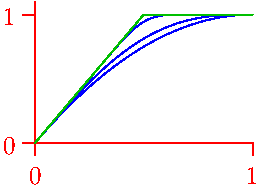
\includegraphics[scale=1]{bernstein}
	\end{minipage}\vspace{-8pt}
	
  \begin{align*}
  B_3f(x)&=f(0)(1-x)^3+3f(\tfrac 13)x(1-x)^2+3f(\tfrac 23)x^2(1-x)+f(1)x^3\\
  &= 0(1-x)^3+ 2x(1-x)^2+3x^2(1-x)+x^3\\
  &=x(2-x)=B_2f(x)\\[5pt]
  B_4f(x)&=0(1-x)^4+2x(1-x)^3+ 6x^2(1-x)^2 +4x^3(1-x)+x^4\\
  &=x(x^3-2x^2+2)
	\end{align*}
	The Bernstein polynomials $B_2f(x), B_4f(x)$ and $B_{50}f(x)$ are drawn.
	
  
  \item Now assume $f(x)=x$ if $x<\frac 12$ and $1-x$ otherwise.\smallbreak
   	\begin{minipage}[t]{0.6\linewidth}\vspace{-20pt}
		\begin{gather*}
  	B_1f(x)=f(0)(1-x)+f(1)x=0\\[5pt]
  	B_2f(x)=x(1-x)\\[5pt]
  	\begin{aligned}
  	B_3f(x)&=0(1-x)^3+x(1-x)^2+x^2(1-x)+0x^3\\
  	&=x(1-x)=B_2f(x)
		\end{aligned}
  	\end{gather*}
	\end{minipage}\begin{minipage}[t]{0.4\linewidth}\vspace{-25pt}
		\flushright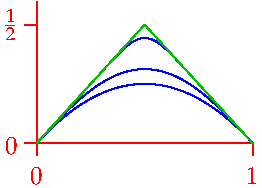
\includegraphics[scale=1]{bernstein2}
	\end{minipage}\vspace{-5pt}
  	\begin{align*}
  	B_4f(x)&=f(0)(1-x)^4+f(\tfrac 14)\!\cdot\! 4x(1-x)^3+f(\tfrac 12)\!\cdot\! 6x^2(1-x)^2 +f(\tfrac 34)\!\cdot\! 4x^3(1-x)+f(1)x^4\\
  	&=x(1-x)^3+3x^2(1-x)^2 +x^3(1-x)\\
  	&=x(1-x)(1+x-x^2)
		\end{align*}
\end{enumerate}
\end{examples}

\clearpage

\def\ray#1{\overrightarrow{#1}}

\boldsubsubsection{Bézier curves (just for fun!)}

\begin{minipage}[t]{0.53\linewidth}\vspace{0pt}
The Bernstein polynomials arise naturally when considering \emph{Bézier curves.} These have many applications, particularly in computer graphics. Given three points $A,B,C$, define points on the line segments $\ray{AB}$ and $\ray{BC}$ for each $t\in[0,1]$, via
\[\ray{AB}(t)=(1-t)A+tB\qquad \ray{BC}(t)=(1-t)B+tC\]
These points move at a constant speed along the corresponding segments. Now consider a \textcolor{blue}{point} on the \textcolor{orange}{\emph{moving} segment} between the points defined above:
\end{minipage}\begin{minipage}[t]{0.47\linewidth}\vspace{0pt}
\flushright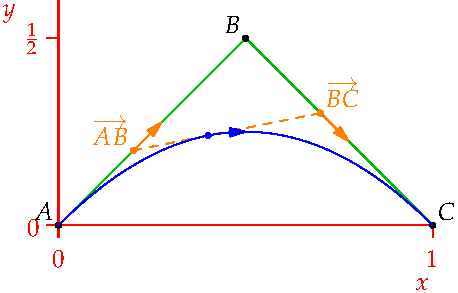
\includegraphics{bezier2}
\end{minipage}\smallbreak

\[R(t):=(1-t)\ray{AB}(t)+t\ray{BC}(t) =(1-t)^2A+2t(1-t)B+t^2C\]
This is the \emph{quadratic Bézier curve with control points $A,B,C$.} The $2^\text{nd}$ Bernstein polynomial for a function $f$ is simply the quadratic Bézier curve with control points $\left(0,f(0)\right)$, $\left(\frac 12,f(\frac 12)\right)$ and $\left(1,f(1)\right)$. The picture\footnote{To see these pictures move, visit \url{https://www.math.uci.edu/~ndonalds/math140b/bezier.html}} above shows $B_2f(x)$ for the above example.\medbreak

We can repeat the construction with more control points: with four points $A,B,C,D$, one constructs $\ray{AB}(t)$, $\ray{BC}(t)$, $\ray{CD}(t)$, then the second-order points between these, and finally the cubic Bézier curve
\begin{align*}
R(t):&=(1-t)\left((1-t)\ray{AB}(t)+t\ray{BC}(t)\right) +t\left((1-t)\ray{BC}(t)+t\ray{CD}(t)\right)\\
&=(1-t)^3A+3t(1-t)^2B+3t^2(1-t)C+t^3D
\end{align*}
where we now recognize the relationship to the $3^\text{rd}$ Bernstein polynomial. 
\begin{center}
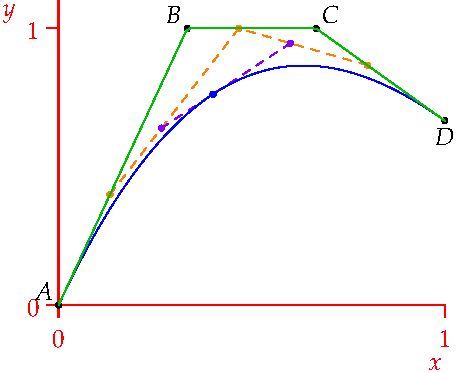
\includegraphics{bezier-cubic2}
\hfill
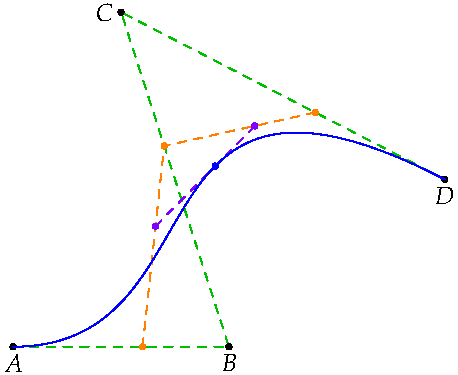
\includegraphics{bezier-cubicalt2}
\end{center}
The pictures show cubic Bézier curves: the first is the graph of the Bernstein polynomial
\[B_3f(x)=0(1-x)^3+3x(1-x)^2+3x^2(1-x)+\tfrac 23x^3\]
while the second is for the four given control points $A,B,C,D$.

\begin{exercises}
	\emph{Key concepts:\quad ?????}

	\begin{enumerate}
	  \item Show that the closed bounded interval assumption in the approximation theorem is required by giving an example of a continuous function $f:(-1,1)\to\R$ which is \emph{not} the uniform limit of a sequence of polynomials.
	  
	  \item If $g:[a,b]\to\R$ is continuous, then $f(x):=g\bigl((b-a)x+a\bigr)$ is continuous on $[0,1]$. If $P_n\to f$ uniformly on $[0,1]$, prove that $Q_n\to g$ uniformly on $[a,b]$, where
		\[Q_n(x)= P_n\left(\frac{x-a}{b-a}\right)\]
	
		\item Use the binomial theorem to check that every Bernstein polynomial for $f(x)=x$ is $B_nf(x)=x$ itself!
	  
		\item Find a parametrization of the cubic Bézier curve with control points $(1,0)$, $(0,1)$, $(-1,0)$ and $(0,-1)$. Now sketch the curve.\\
		(\emph{Use a computer algebra package if you like!})
		
		\item (Hard) Show that the Bernstein polynomials for $f(x)=x^2$ are given by 
		\[B_nf(x)=\frac 1nx+\frac{n-1}nx^2\]
		and thus verify explicitly that $B_nf\to f$ uniformly.
	\end{enumerate}
\end{exercises}

\fi

\graphicspath{{3diff/asy/}}

\section{Differentiation}

Differentiation grew out of the problem of \emph{instantaneous velocity.} Velocity can only easily be measured as an \emph{average} over a time interval:\footnote{%
	Even a modern technique such as Doppler-shift compares measurements separated by the extremely small period of a light or soundwave. These are still therefore \emph{average} velocities, albeit taken over very small time intervals.%
}
if an object travels $\Delta d$ meters in $\Delta t$ seconds, then its average velocity is $v_\text{av}=\frac{\Delta d}{\Delta t}$ ms$^{-1}$. An early `definition' (dating to the 1300s) makes the instantaneous velocity equal to the constant velocity that would be observed if a body were to stop accelerating: while useless for the purposes of measurement, this is essentially Newton's first law regarding inertial motion (1687). We also see the concept of the \emph{tangent line} beginning to appear. Indeed if one graphs position against time, intuition tells us:
\begin{itemize}
  \item The graph of inertial (constant speed) motion is a straight line whose slope is the velocity.
  \item The tangent line to a curve has slope equal to the instantaneous velocity. 
\end{itemize}
The problem of finding, defining and computing instantaneous velocity thus morphed into the consideration of tangent lines to curves. With the advent of analytic geometry in the early 1600s, mathematicians such as Fermat and Descartes pioneered versions of the familiar \emph{secant (`cutting') line} method for computing tangents.

\begin{center}
	\begin{tabular}{p{0.46\linewidth}@{\qquad}p{0.46\linewidth}}
		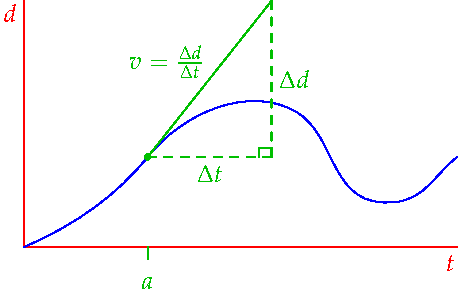
\includegraphics{diff-history}
		&
		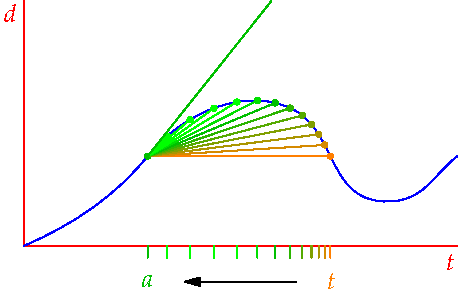
\includegraphics{diff-history2}
		\\
		\centering Instantaneous velocity equals constant velocity corresponding to tangent line
		&
		\centering Secant lines approximate tangent line as $t\to a$
	\end{tabular}
\end{center}

The average velocity of the particle over the time interval $[a,t]$ is the slope of the secant line, namely
\[
	v_\text{av}(a,t)=\frac{d(t)-d(a)}{t-a}
\]
Since the secant lines approximate the tangent line as $t$ approaches $a$, it seems  reasonable that we should compute the instantaneous velocity in this manner:
\[
	v(a)=\lim_{t\to a}v_\text{av}(a,t)
	=\lim_{t\to a}\frac{d(t)-d(a)}{t-a}
\]
This is, of course, the modern definition of the \emph{derivative.}
\goodbreak


\setcounter{subsection}{27}
\subsection{Basic Properties of the Derivative}\label{sec:derivproperties}

\begin{defn}{}{deriv}
	Let $f:U\to\R$ and $a\in U$. We say that \emph{$f$ is differentiable at $a$} if the following limit exists (is \emph{finite}!)
	\[
		\lim_{x\to a}\frac{f(x)-f(a)}{x-a}
	\]
	We call this limit the \emph{derivative of $f$ at $a$} and denote its value by $\diffat[f]{x}{x=a}$ or $f'(a)$.\smallbreak
	If $f'(a)$ exists for all $a\in U$ then $f$ is \emph{differentiable (on $U$)}; the derivative becomes a function $\textcolor{Green}{f'(x)}=\textcolor{red}{\diff[f]{x}}$.
\end{defn}

The two notations are partly attributable to the primary founders of calculus: \textcolor{Green}{Issac Newton} and \textcolor{red}{Gottfried Leibniz}. Each has its pros and cons and you should be comfortable with both.

\boldinline{One-sided derivatives} Since the defining limit is \emph{two-sided,} differentiability only makes sense at \emph{interior points} of $U$. \emph{Left-} and \emph{right-derivatives} may be defined using one-sided limits; differentiability is  equivalent to these being equal. All results in this section hold for one-sided derivatives with suitable (sometimes tedious) modifications. It is common, though strictly incorrect, to say that $f$ is differentiable on $[a,b)$ if it is differentiable on the interior $(a,b)$ and \emph{right-}differentiable at $a$. In these notes we will strictly adhere to Definition \ref{defn:deriv}: differentiable means \emph{two-sided.}


\begin{examples}{}{}
	Basic examples should be familiar from elementary calculus.
	\begin{enumerate}
	  \item Let $f(x)=x^2+4x$. Then, for any $a\in\R$,
		\begin{align*}
			\lim_{x\to a}\frac{f(x)-f(a)}{x-a}
			&=\lim_{x\to a}\frac{x^2+4x-a^2-4a}{x-a} 
			=\lim_{x\to a}\frac{(x-a)(x+a+4)}{x-a}\\
			&=\lim_{x\to a}(x+a+4)=2a+4
		\end{align*}
		Note how the definition of $\lim\limits_{x\to a}$ allows us to cancel the $x-a$ terms from the numerator and denominator. We conclude that $f$ is differentiable (on $\R$) and that $f'(x)=2x+4$.
		
		\item Let $g(x)=\frac{x+1}{2x-3}$. Then, for any $a\neq\frac 32$,
		\begin{align*}
			\lim_{x\to a}\frac{f(x)-f(a)}{x-a}
			&=\lim_{x\to a}\frac 1{x-a}\left[\frac{x+1}{2x-3}-\frac{a+1}{2a-3}\right] 
			=\lim_{x\to a}\frac{5a-5x}{(x-a)(2x-3)(2a-3)}\\
			&=\lim_{x\to a}\frac{-5}{(2x-3)(2a-3)} 
			=\frac{-5}{(2a-3)^2}
		\end{align*}
		$f$ is therefore differentiable on its domain $\R\setminus\{\frac 32\}$ with derivative $f'(x)=\frac{-5}{(2x-3)^2}$.
	\end{enumerate}
\end{examples}

The familiar expressions
\[
	f'(a)=\lim_{h\to 0}\frac{f(a+h)-f(a)}h,\qquad 
	f'(x)=\lim_{h\to 0}\frac{f(x+h)-f(x)}h
\]
are equivalent to the original definition (see Exercise \ref{ex:hderiv}). While seemingly simpler, they sometimes lead to nastier calculations: see what happens if you try the previous example in this language\ldots\medbreak\goodbreak

We now turn to possibly the most well-known result of Freshman Calculus.

\begin{thm}{Power Law}{}
	Let $r\in\R$. Then $f(x)=x^r$ is differentiable with $f'(x)=rx^{r-1}$.
\end{thm}

The domains of $f$ and $f'$ depend messily on $r$, but the above certainly holds on the interval $(0,\infty)$. We leave a complete proof to the exercises and instead consider a few generalizable examples.

\begin{examples}{}{}
\exstart If $n\in\N$ and $a\in\R$, a simple factorization yields
\begin{align*}
	\lim_{x\to a}\frac{x^n-a^n}{x-a}&=\lim_{x\to a}\frac{(x-a)(x^{n-1}+ax^{n-2}+\cdots +a^{n-2}x+a^{n-1})}{x-a}\tag{$\ast$}\\
	&=\lim_{x\to a}(x^{n-1}+ax^{n-2}+\cdots +a^{n-2}x+a^{n-1}) =na^{n-1}
	\end{align*}
We conclude that $\diff x x^n=nx^{n-1}$.
\begin{enumerate}\setcounter{enumi}{1}
	\begin{minipage}[t]{0.7\linewidth}\vspace{0pt}
		\item If \textcolor{blue}{$f(x)=x^{-1}$} and $a\neq 0$, then
		\begin{align*}
			\lim_{x\to a}\frac{x^{-1}-a^{-1}}{x-a}&=\lim_{x\to a}\frac{a-x}{ax(x-a)} =\lim_{x\to a}\frac{-1}{ax}=-\frac 1{a^2}
		\end{align*}
		from which we conclude that \textcolor{Green}{$f'(x)=-x^{-2}$}.\smallbreak
		A similar approach followed by the factorization ($\ast$) proves the power law for all 	negative integer exponents:
		\[\frac{x^{-n}-a^{-n}}{x-a}=\frac{a^n-x^n}{a^nx^n(x-a)}=\cdots\]
	\end{minipage}\begin{minipage}[t]{0.3\linewidth}\vspace{-10pt}
		\flushright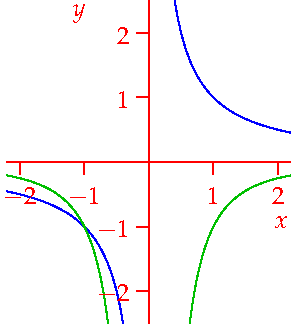
\includegraphics[scale=0.9]{diff-exneg2}
	\end{minipage}\bigbreak


	\begin{minipage}[t]{0.7\linewidth}\vspace{0pt}
		\item To differentiate $x^{1/n}$, simply substitute $x=y^n$ and observe case 1. If \textcolor{purple}{$g(x)=x^{1/3}$} and $a\neq 0$, then $y=x^{1/3}$ and $b=a^{1/3}$ yield
		\begin{align*}
			\lim_{x\to a}\frac{x^{1/3}-a^{1/3}}{x-a}&= \lim_{y\to b}\frac{y-b}{y^3-b^3} = \frac 1{3b^2}=\frac 13a^{-2/3}\\
			&\implies \textcolor{orange}{g'(x)=\frac 13x^{-2/3}}
		\end{align*}
		Note that $g$ is \emph{not} differentiable at $x=0$!
	\end{minipage}\begin{minipage}[t]{0.3\linewidth}\vspace{0pt}
		\flushright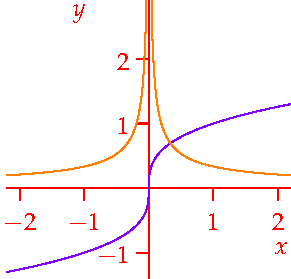
\includegraphics[scale=0.9]{diff-exthird}
	\end{minipage}
\end{enumerate}
\hangindent0pt We could similarly compute the derivative for all rational exponents, though it is much easier to wait for the chain rule. The power law for irrational exponents is somewhat more ticklish.
\end{examples}





\begin{cor}{Basic Transcendental Functions}{}
Recalling our development of power series in the previous chapter, the power law (for positive integers!) is all we need to see that
\[\diff x\exp(x)=\exp(x),\qquad \diff x\sin x=\cos x,\qquad \diff x\cos x=-\sin x\]
\end{cor}

It is also possible to develop these results independently of power series (see e.g.\ Exercise \ref{ex:trigdiff}).
\goodbreak


\boldsubsubsection{Failure of differentiability} It is instructive to consider when a function can fail to be differentiable. First a simple result shows that functions are not differentiable at discontinuities.

\begin{thm}{}{}
If $f$ is differentiable %\footnote{Similarly right/left-differentiability implies right/left-continuity.}
 at $a$ then $f$ is continuous at $a$.
\end{thm}

\begin{proof}
Simply take the limit (think carefully why this works!):
\[\lim_{x\to a}f(x)=\lim_{x\to a}\left[\frac{f(x)-f(a)}{x-a}(x-a)+f(a)\right] =f'(a)(0-0)+f(a) =f(a)\tag*{\qedhere}\]
%The first term approaches $f'(a)\cdot\lim\limits_{x\to a}(x-a)=0$ since $f'(a)$ is defined and finite.
\end{proof}

It remains to consider situations when a function is continuous but not differentiable.

\begin{examples}{}{}
The following cover all situations where a function is continuous on an interval and differentiable everywhere \emph{except} at a single interior point; similarly to isolated discontinuities, these are classified by considering the three ways in which the derivative limit might not exist. 
\begin{enumerate}
	\item A \emph{vertical tangent line} occurs when the derivative is infinite. For instance, $g(x)=x^{1/3}$ at $x=0$. 
  \item \emph{Corners} occur when the one-sided derivatives are unequal (could be infinite). For instance, $f(x)=\nm x$ is not differentiable at zero, the one-sided derivatives being
  \begin{gather*}
  \lim_{x\to 0^+}\frac{\nm x-\nm 0}{x-0}=\lim_{x\to 0^+}\frac xx =1\neq
  \lim_{x\to 0^-}\frac{\nm x-\nm 0}{x-0}=\lim_{x\to 0^-}\frac{-x}x =-1
  \end{gather*}
	Indeed $f$ is differentiable everywhere except at zero, with
  \[f'(x)=\begin{cases}
	1&\text{if }x>0\\
	-1&\text{if }x<0
	\end{cases}\]

	\begin{minipage}[t]{0.65\linewidth}\vspace{0pt}
  \item A \emph{singularity} is where left- and/or right-derivatives do not exist. The standard example in this case is
  \[f(x)=\begin{cases}
  x\sin\frac 1x&\text{if }x\neq 0\\
  0&\text{if }x=0
  \end{cases}\]
  which is continuous on $\R$ and differentiable everywhere except at zero: the details are in Exercise \ref{ex:diffnonzero}.
  \end{minipage}\begin{minipage}[t]{0.35\linewidth}\vspace{0pt}
  \flushright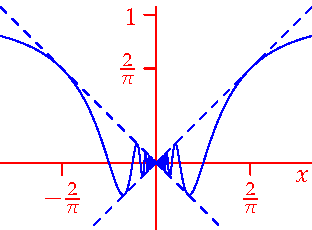
\includegraphics[scale=0.9]{unifcontex2}
  \end{minipage}
\end{enumerate}
\hangindent0pt Singularities and vertical tangent lines can also prevent one-sided differentiability.
\end{examples}

More esoteric examples of non-differentiability are also possible:
\begin{itemize}
  \item Utilizing series, we can create functions which are continuous on an interval but \emph{nowhere differentiable}! For a classic example, see page \ref{strangefunction}.
  \item It is also possible to construct a function which differentiable (and thus continuous) at precisely one point; can you think of an example?
\end{itemize}

\goodbreak


\boldsubsubsection{The Basic Rules of Differentiation}
	
\begin{thm}{}{basicdiff}
Let $f,g$ be differentiable and $k,l$ be constants.
\begin{enumerate}
  \item (Linearity)\quad The function $kf+lg$ is differentiable with $(kf+lg)'=kf'+lg'$.
  \item (Product rule)\quad The function $fg$ is differentiable with $(fg)'=f'g+fg'$.
  \item (Inverse functions)\quad If $f$ is bijective with non-zero derivative, then $f^{-1}$ is differentiable and
	\[\diff xf^{-1}(x)=\frac 1{f'\big(f^{-1}(x))\big)}\] 
\end{enumerate}
\end{thm}

\begin{proof}
Parts 1 and 2 follow from the limit laws:
\begin{gather*}
\lim_{x\to a}\frac{(kf+lg)(x)-(kf+lg)(a)}{x-a}=\lim_{x\to a}\left[k\frac{f(x)-f(a)}{x-a}+l\frac{g(x)-g(a)}{x-a}\right]=kf'(a)+lg'(a)\\
\lim_{x\to a}\frac{f(x)g(x)-f(a)g(a)}{x-a}=\lim_{x\to a}\left[\frac{f(x)-f(a)}{x-a}g(x)+f(a)\frac{g(x)-g(a)}{x-a}\right]=f'(a)g(a)+f(a)g'(a)
\end{gather*}
Note where we used the continuity of $g$ in the second line ($\lim g(x)=g(a)$). Part 3 is an exercise.
\end{proof}

The inverse function rule is intuitive since the graphs of $f$ and $f^{-1}$ are related by reflection in the line $y=x$; gradients at corresponding points are therefore reciprocal. In Leibniz notation the result reads $\diff[x]{y}=\left(\diff[y]{x}\right)^{-1}$.

\begin{examples}{}{}
\hangindent\leftmargin
\textup{1. } Linearity allows us to differentiate any polynomial: for instance
	\[\diff x\big(7x^2+13x^4\big)=7\diff xx^2+13\diff xx^4=14x+52x^3\]
\begin{enumerate}\setcounter{enumi}{1}
	\item The product rule extends the reach of differentiation somewhat:
	\[\diff x(x^4\sin x) =\left(\diff xx^4\right)\sin x+x^4\diff x\sin x = 4x^3\sin x-x^4\cos x\]
	\item The inverse trigonometric functions can now be differentiated. For instance,
	\[y=\sin^{-1}x\implies \diff x\sin^{-1}x=\diff[y]{x}=\left(\diff[x]{y}\right)^{-1}=\frac 1{\cos y}=\frac 1{\sqrt{1-\sin^2\!y}}=\frac 1{\sqrt{1-x^2}}\]
	%We chose the positive square-root since arcsine is, by convention, increasing. %Clearly arcsine is only differentiable on the open interval $(-1,1)$; indeed it has vertical tangent lines at $\pm 1$.
	
	\item Define natural log to be the inverse of the (bijective!) exponential function $\exp(x)$:
	\[y=\ln x\iff x=\exp y\]
	It follows that
	\[\diff x\ln x=\left(\diff[x]{y}\right)^{-1}=\frac 1{\exp y}=\frac 1x\]
	The full details, and the justification that $\exp x=e^x$, form an optional exercise.
\end{enumerate}
\end{examples}\goodbreak


\begin{thm}{Chain Rule}{}
If $g$ is differentiable at $a$ and $f$ is differentiable at $g(a)$ then $f\circ g$ is differentiable at $a$ with derivative
\[(f\circ g)'(a)=f'\big(g(a)\big)\,g'(a)\]
\end{thm}

In Leibniz notation this reads $\diff[(f\circ g)]{x}=\diff[f]{g}\diff[g]{x}$ which looks like a simple cancellation of the $\dg$ terms!\footnote{
This is completely unjustified since $\dg$ does not (for us) mean anything on its own! The same problem appears in the famously faulty one-line `proof' of the chain rule:
\[\lim_{x\to a}\frac{f\big(g(x)\big)-f\big(g(a)\big)}{x-a} \overset{\text{?}}{=} \lim_{x\to a}\frac{f\big(g(x)\big)-f\big(g(a)\big)}{g(x)-g(a)} \lim_{x\to a}\frac{g(x)-g(a)}{x-a}\]
The second limit cannot exist unless $g(x)\neq g(a)$ for all $x$ near, but not equal to, $a$. The faulty argument is repaired by replacing the second difference quotient with $f'\big(g(a))$ whenever $g(x)=g(a)$, \emph{before} taking the limit. This is precisely what $\gamma\bigl(g(x)\bigr)$ does in the correct proof.}



\begin{proof}
Define $\gamma:\dom(f)\to\R$ via
\[\gamma(v)=\begin{cases}
\frac{f\big(v\big)-f\big(g(a)\big)}{v-g(a)}&\text{if }v\neq g(a)\\
f'\big(g(a)\big)&\text{if }v=g(a)
\end{cases} \tag{$\ast$}\]
Since $f$ is differentiable at $g(a)$, we see that $\gamma$ is continuous and \smash[b]{$\lim\limits_{v\to g(a)}\gamma(v)=f'\bigl(g(a)\bigr)$.}\medbreak
Since $g$ is differentiable at $a$, there exists an open interval $U\ni a$ for which $x\in U\implies g(x)\in\dom(f)$.\smallbreak
Now compute: for any $x\in U\setminus\{a\}$, let $v=g(x)$ in ($\ast$), whence
\[\frac{f\big(g(x)\big)-f\big(g(a)\big)}{x-a}=\gamma\bigl(g(x)\bigr)\frac{g(x)-g(a)}{x-a}\]
Take limits as $x\to a$ for the result.
\end{proof}

\begin{cor}{Quotient Rule}{quotinv1}
Suppose $f$ and $g$ are differentiable. Then $\frac fg$ is differentiable whenever $g(x)\neq 0$. Moreover
\[\left(\frac fg\right)'=\frac{f'g-fg'}{g^2}\]
\end{cor}

The proof is an exercise.


% \begin{proof}
% Recalling that $\diff x x^{-1}=-x^{-2}$, apply the chain rule to obtain $\diff x\frac 1{g(x)}=-\frac{g'(x)}{g(x)^2}$. Now apply the product rule to $f\cdot\frac 1g$.
% \end{proof}

% \begin{proof}
% Simply apply the chain rule to $f(g(x))=x$ where $g=f^{-1}$.
% \end{proof}



\begin{examples}{}{}
\exstart By the quotient rule,
	\[\diff x\tan x=\diff x\frac{\sin x}{\cos x}=\frac{\cos^2\!x+\sin^2\!x}{\cos^2\!x}=\sec^2\!x\]
\begin{enumerate}\setcounter{enumi}{1}
	\item We can now differentiate highly involved combinations of elementary functions:
	\[\diff x\left[\tan(e^{4x^2})-\frac{7x}{\sin x}\right]=8xe^{4x^2}\sec^2(e^{4x^2})-\frac{7\sin x-7x\cos x}{\sin^2\!x}\]
\end{enumerate}
\end{examples}

\vfil

\begin{exercises}{}
\exstart Use Definition \ref{defn:deriv} to calculate the derivatives.
\begin{enumerate}\setcounter{enumi}{1}
% 	\item[]\begin{enumeratea}
%     \item $f(x)=x^3$ \ at $x=2$.\qquad\qquad\qquad\ \text{(b)}\ \ $g(x)=x+2$ \ at $x=a$.\vspace{2pt}
%     \item[(c)] $f(x)=x^2\cos x$ \ at $x=0$.\qquad\qquad \text{(d)}\ \ $r(x)=\dfrac{3x+4}{2x-1}$ \ at $x=1$.
%   \end{enumeratea}
  

	\item[]\begin{enumeratea}
	  \item \makebox[170pt][l]{$f(x)=x^3$ \ at $x=2$ \hfill(b)}
		\space $g(x)=x+2$ \ at $x=a$
		\item[(c)] \makebox[170pt][l]{$f(x)=x^2\cos x$ \ at $x=0$ \hfill(d)}
		\space $r(x)=\dfrac{3x+4}{2x-1}$ \ at $x=1$
	\end{enumeratea}
  
  \item Differentiate the function $f(x)=\cos\left(e^{x^5-3x}\right)$ using the chain and product rules.
  
  \item\begin{enumerate}
    \item Prove the quotient rule (Corollary \ref{cor:quotinv1}) by combining the chain and product rules.
  	\item Prove the inverse derivative rule (Theorem \ref{thm:basicdiff}, part 3).\smallbreak
  	(\emph{Hint: You can't simply differentiate $1=\diff[x]x=\diff xf(f^{-1}(x))$ using the chain rule; why not?})
  \end{enumerate}
  
  
  
  \item\begin{enumerate}
    \item Find the derivatives of secant, cosecant and cotangent using the quotient rule.
    \item Why did we choose the positive square-root when computing $\diff x\sin^{-1}x$? What is the standard domain of arcsine, and what happens at $x=\pm 1$?
    \item Find the derivatives of the inverse trigonometric functions using the inverse function rule.
  \end{enumerate}
  
  \item\label{ex:hderiv} Using the definition of the derivative, and supposing that $f$ is differentiable at $a$, prove that
  \[f'(a)=\lim_{h\to 0}\frac{f(a+h)-f(a)}{h}=\lim_{h\to 0}\frac{f(a+h)-f(a-h)}{2h}\]
  
%   \item Use induction to prove the power law $\diff xx^n=nx^{n-1}$ when $n\in\N$ using \emph{only} the following:
%   \begin{enumerate}
%     \item $\diff xx=1$
%     \item The product rule
%   \end{enumerate}
  
  \item Prove that the function $f(x)=x\nm x$ is differentiable everywhere and compute its derivative.
  
  
  \item\label{exs:diffdiscont} Show that following function is differentiable everywhere and compute its derivative:
  \[f(x)=\begin{cases}
  x^2\sin\frac 1x&\text{if }x\neq 0\\
  0&\text{if }x=0
  \end{cases}\]
  Moreover, prove that the derivative $f'$ is \emph{discontinuous} at $x=0$.
  
  \item\label{ex:diffnonzero} Show that the following function is differentiable everywhere \emph{except} at zero:
  \[f(x)=\begin{cases}
  x\sin\frac 1x&\text{if }x\neq 0\\
  0&\text{if }x=0
  \end{cases}\]
  

	\begin{minipage}[t]{0.63\linewidth}\vspace{0pt}
	  \item\label{ex:trigdiff}\begin{enumerate}
	    \item Suppose $0<h<\frac\pi 2$. Use the picture to show that
			\[0<\frac{1-\cos h}h< \sin\frac{h}2 \quad\text{and}\quad  \sin h< h<\tan h\]
			Hence conclude that $\lim\limits_{h\to 0}\frac{\sin h}h=1$ and $\lim\limits_{h\to 0}\frac{1-\cos h}h=0$.
		\item Use part (a) to prove that $\diff x\sin x=\cos x$
	\end{enumerate}
	\end{minipage}\begin{minipage}[t]{0.37\linewidth}\vspace{0pt}
  \flushright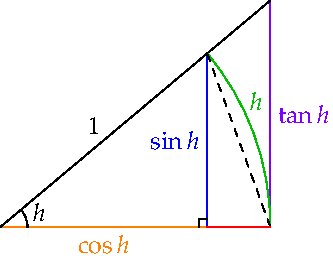
\includegraphics[scale=1]{trig-diff2}
  \end{minipage}
	
   \item (Hard) Use induction to prove the Leibniz rule (general product rule):
   \[(fg)^{(n)}=\sum_{k=0}^n\binom nkf^{(k)}g^{(n-k)}\]
\end{enumerate}
\end{exercises}

\clearpage

\begin{tcolorbox}[exercisestyle,title={\large Masochists Corner (non-examinable)\smallbreak}]

We finish with two \emph{very hard} bonus exercises, though the first is somewhat easier. If you want a challenge, give 'em a go!

\begin{description}
  \item[The Exponential Function \& the General Power Law]\phantom{bob}\smallbreak

  Consider the function $\exp(x):=\sum\limits_{n=0}^\infty\dfrac{x^n}{n!}$ which converges for all real $x$.\\
  As we saw when discussing power series, this function satisfies the initial value problem
  \[\diff x\exp(x)=\exp(x),\qquad \exp(0)=1\]
	\emph{Define} $e:=\exp(1)$. Certainly $e^x$ makes sense whenever $x\in\Q$. When $x$ is  irrational, define
	  \[e^x:=\sup\{e^q:q\in\Q,\ q< x\}\]
	Our primary goal is to \emph{prove} that $\exp(x)=e^x$. As a nice bonus we recover Bernoulli's limit identity $e=\lim\limits_{n\to\infty}\left(1+\frac 1n\right)^n$ and obtain a complete proof of the power law. 
  \begin{enumeratea}
    \item For all $x,y\in\R$, prove that $\exp(x+y)=\exp(x)\exp(y)$\smallbreak
    (\emph{Hint: use the binomial theorem and change the order of summation})
    \item Show that $\exp(x)$ is always positive, \emph{even when $x<0$.}
    \item Prove that $\exp:\R\to (0,\infty)$ is bijective.\smallbreak
    (\emph{Hint: $x\ge 0\implies \exp(x)\ge 1+x$; take limits then apply part (a)})
    \item Prove that $e^x=\exp(x)$. Do this in three stages:
    \begin{itemize}
      \item If $x\in\N$, use part (a). Now check for $x\in\Z^-$.
      \item If $x=\frac mn\in\Q$, first compute $\left[\exp(\frac mn)\right]^n$.
      \item If $x$ is irrational, start with $\exists (q_n)\subseteq\Q$ such that $q_n<x$ and $e^{q_n}\to e^x$\ldots
    \end{itemize}

    \item Let $\ln:(0,\infty)\to\R$ be the inverse function of $\exp$. Prove the logarithm laws:
    \[\ln(xy)=\ln x+\ln y\quad\text{and}\quad \ln x^r=r\ln x\]
    (\emph{Just do this when $r\in\N$; another argument like part (d) is required in general})
    \item We've already seen that $\diff y\ln y=\frac 1y$. Use the fact that
    \[\diff y\ln y=\lim_{h\to 0}\frac{\ln(y+h)-\ln y}h\]
    to prove that $\exp(x)=\lim\limits_{n\to\infty}\left(1+\frac xn\right)^n$, thus recovering Bernoulli's definition of $e$.
		\item For any $r\in\R$, \emph{define} $x^r:=\exp(r\ln x)$. Hence obtain the power law for any exponent.
   \end{enumeratea}
\end{description}
\end{tcolorbox}
   
   \vfill
   
	\goodbreak
	
	\begin{tcolorbox}[exercisestyle,title={}]
\begin{description}
   \item[A Very Strange Function]\phantomsection\label{strangefunction}\phantom{bob}\smallbreak
   
   Here is a classic example of a continuous but nowhere-differentiable function!\smallbreak

Let $f$ be the \emph{sawtooth} function defined by \textcolor{Green}{$f(x)=\nm x$} whenever $x\in[-1,1]$ and extending periodically to $\R$ so that \textcolor{Green}{$f(x+2)=f(x)$}. Now define $\textcolor{blue}{g}:\R\to\R$ via
  \[\textcolor{blue}{g(x)=\sum_{n=0}^\infty \left(\frac 34\right)^nf(4^nx)}\]
  \vspace{-30pt}
  \begin{center}
  \begin{tabular}{c@{\qquad}c}
  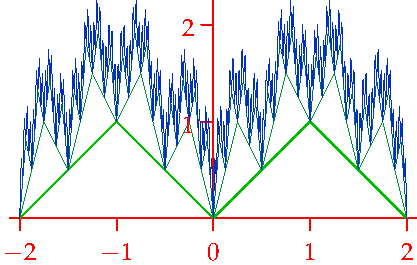
\includegraphics{sawtooth}&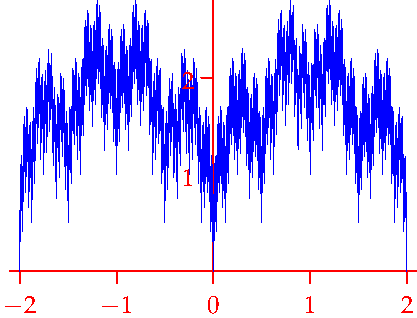
\includegraphics{sawtooth2}\\
  $f(x)$ and iterations to $n=3$
  &$g(x)$ (really $n=6$, but can you tell?!)
  \end{tabular}
  \end{center}
  
  \begin{enumeratea}
    \item Prove that $g$ is well-defined and continuous on $\R$.
    \item Let $x\in\R$ and $m\in\N$ be fixed. Define $h_m=\pm\frac 12\cdot 4^{-m}$ where the $\pm$-sign is chosen so that no integers lie strictly between $4^mx$ and $4^m(x+h_m)=4^mx\pm\frac 12$.\smallbreak
    For each $n\in\N_0$, define
    \[k_n =\frac{f\big(4^n(x+h_m)\big)-f(4^nx)}{h_m}\]
    Prove the following
    \begin{enumerate}
      \item[i.] $\nm{k_n}\le 4^n$ with equality when $n=m$.
      \item[ii.] $n>m\implies k_n=0$.
    \end{enumerate}
    (\emph{Hint: $\nm{f(y)-f(z)}\le\nm{y-z}$: when is this an equality?})

    \item Use part (b) to prove that
    \[\nm{\frac{g(x+h_m)-g(x)}{h_m}}\ge \frac 12(3^m+1)\]
    Hence conclude that $g$ is \emph{nowhere differentiable.}
  \end{enumeratea}
\end{description}

\end{tcolorbox}
	
\clearpage

\subsection{The Mean Value Theorem}\label{sec:mvt}

We now turn to one of the central results in calculus.

\begin{thm}{Mean Value Theorem/MVT}{}
Let $f$ be continuous on $[a,b]$ and differentiable on $(a,b)$. Then there exists $\xi\in(a,b)$ such that $\textstyle f'(\xi)=\frac{f(b)-f(a)}{b-a}$.
\end{thm}

This follows easily from two lemmas.

\begin{lemm}{}{rolle}
\exstart (Critical Points)\quad Suppose $g$ is bounded on $(a,b)$ and attains its maximum or minimum at $\xi\in(a,b)$. If $g$ is differentiable at $\xi$ then $g'(\xi)=0$. \vspace{-5pt} %If $g$ is differentiable at $\xi$ then $g'(\xi)=0$.
\begin{enumerate}\setcounter{enumi}{1}\itemsep0pt
  \item (Rolle's Theorem)\quad Suppose $g$ is continuous on $[a,b]$, differentiable on $(a,b)$, and that $g(a)=g(b)$. Then there exists $\xi\in(a,b)$ such that $g'(\xi)=0$. 
\end{enumerate}
\end{lemm}

The main result follows by applying Rolle's theorem to
\[g(x)=f(x)-\frac{f(b)-f(a)}{b-a}(x-b)\]
and observing that $g(a)=f(b)=g(b)$ and $g'(x)=f'(x)-\frac{f(b)-f(a)}{b-a}$.

\begin{center}
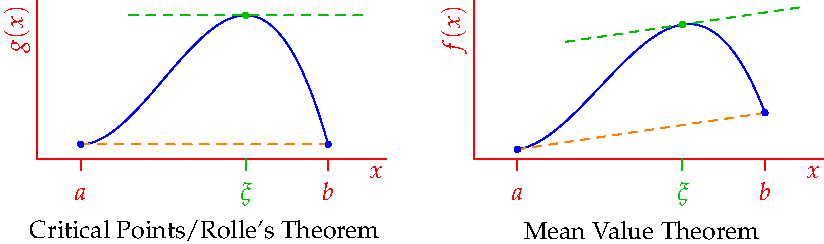
\includegraphics{mvt}
\end{center}

In the pictures, the orange and green lines are \emph{parallel}: the \textcolor{orange}{average slope} over the interval $[a,b]$ equals the \textcolor{Green}{gradient/derivative} $f'(\xi)$.

\begin{proof}[Proof of Lemma]
\begin{enumerate}\itemsep0pt
  \item Suppose, for a contradiction, that
	\[g'(\xi)=\lim_{x\to \xi}\frac{g(x)-g(\xi)}{x-\xi}>0\]
	Let $\epsilon=g'(\xi)$ in the definition of limit: $\exists\delta>0$ such that
	\[0<\nm{x-\xi}<\delta\implies\nm{\frac{g(x)-g(\xi)}{x-\xi}-g'(\xi)}<g'(\xi)\implies 0<\frac{g(x)-g(\xi)}{x-\xi}<2g'(\xi)\]
	In particular, if $x\in(\xi,\xi+\delta)$, then $g(x)>g(\xi)$, contradicting the maximality at $\xi$.\smallbreak
	The argument when $g'(\xi)<0$ is similar. Finally, apply to $-g$ for the result at a minimum.
  \item By the extreme value theorem, $g$ is bounded and attains its bounds.
  If the maximum and minimum \emph{both} occur at the endpoints $a,b$, then $g$ is constant: any $\xi\in(a,b)$ satisfies the result.
Otherwise, at least one extreme value occurs at some $\xi\in(a,b)$: part 1 says that $g'(\xi)=0$.\hfill\qedhere
\end{enumerate}
\end{proof}\goodbreak

\begin{examples}{}{}
\exstart Let $f(x)=(x-1)^2(4-x)+x$ on $[a,b]=[1,4]$: this is roughly the above picture illustrating the mean value theorem. We compute the average slope and the derivative:
	\[\frac{f(b)-f(a)}{b-a}=1,\qquad f'(x)=2(x-1)(4-x)-(x-1)^2+1 =-3x^2+12x-8\]
	and observe that
	\[f'(\xi)=\frac{f(b)-f(a)}{b-a}\iff 3\xi^2-12\xi+9=0\iff \xi=1\text{ or }3\]
	Since only 3 lies in the interval $(1,4)$, this is the value $\xi$ satisfying the mean value theorem.
\begin{enumerate}\setcounter{enumi}{1}
  \item We find the maximum and minimum values of $g(x)=x^4-14x^2+24x$ on the interval $[0,2]$.\vspace{-8pt}
  
  \begin{minipage}[t]{0.68\linewidth}\vspace{0pt}
  The function is differentiable, with
  \[g'(x)=4x^3-28x+24=4(x-2)(x-1)(x+3)\]
  By the Lemma, the locations of the extrema are either the endpoints $x=0,2$ or locations with zero derivative ($x=1$). Since
  \[f(0)=0,\quad f(1)=11,\quad f(2)=8\]
  we conclude that $\max(f)=f(1)=11$ and $\min(f)=f(0)=0$.
  \end{minipage}\begin{minipage}[t]{0.32\linewidth}\vspace{0pt}
  \flushright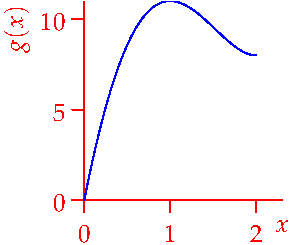
\includegraphics{mvt-ex}
  \end{minipage}
%   
% 	\item Many values of $\xi$ can satisfy the Mean Value or Rolle's Theorem. For instance, if $f(x)=\sin x$ on the interval $[0,10\pi]$, then
% 	\[\frac{f(10\pi)-f(0)}{10\pi-0}=\cos \xi=f'(\xi) \iff \xi=\frac\pi 2,\frac{3\pi}2,\ldots,\frac{19\pi}2\]
\end{enumerate}
\end{examples}

\boldinline{Consequences of the Mean Value Theorem} Several simple corollaries relate to monotonicity.

\begin{defn}{}{}
Suppose $f:I\to\R$ is defined on an interval $I$. We say that $f$ is:\vspace{-5pt}
\begin{description}\itemsep0pt
  \item[\normalfont\emph{Increasing (monotone-up) on $I$}] if $x<y\implies f(x)\le f(y)$
  \item[\normalfont\emph{Decreasing (monotone-down) on $I$}] if $x<y\implies f(x)\ge f(y)$
\end{description}\vspace{-5pt}
We say \emph{strictly} increasing/decreasing if the inequalities are strict.
\end{defn}

\begin{examples}[lower separated=false, sidebyside, sidebyside align=top seam, sidebyside gap=0pt, righthand width=0.4\linewidth]{}{}
\exstart $f:x\mapsto x^2$ is strictly increasing on $[0,\infty)$ and strictly decreasing on $(-\infty,0]$.
\begin{enumerate}\setcounter{enumi}{1}
	\item The floor function $f:x\mapsto \lfloor x\rfloor$ (the greatest integer less than or equal to $x$) is increasing, but not strictly, on $\R$.
\end{enumerate}
\tcblower
  \flushright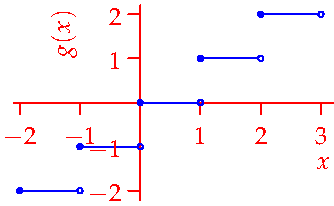
\includegraphics{mvt-floor}
\end{examples}

\begin{cor}{}{mvtincdec}
Suppose $f$ is differentiable on an interval $I$, then
\begin{enumerate}\itemsep0pt
  \item $f'\ge 0\text{ on }I\iff f\text{ is increasing on }I$
  \item $f'\le 0\text{ on }I\iff f\text{ is decreasing on }I$
  \item $f'=0\text{ on }I\iff f\text{ is constant on }I$
\end{enumerate}
\end{cor}
\vfil
\pagebreak

\begin{proof}
($\Rightarrow$)\quad Let $x<y$ where $x,y\in I$. By the mean value theorem, $\exists\xi\in(x,y)$ such that
\[\frac{f(y)-f(x)}{y-x}=f'(\xi)\quad\text{whence}\quad f'(\xi)\ge 0\implies f(y)\ge f(x)\]
($\Leftarrow$)\quad For the converse, use the definition of derivative: \smash{$f'(\xi)=\lim\limits_{x\to\xi}\frac{f(x)-f(\xi)}{x-\xi}$.} If $f$ is increasing, then
\[x>\xi\implies f(x)\ge f(\xi)\implies f'(\xi)\ge 0\]
Parts 2 and 3 are similar.
\end{proof}

Corollary \ref{cor:mvtincdec} yields a couple of flashbacks to elementary calculus.

\begin{cor}{}{1stderivtest}
Let $I$ be an interval.
\begin{enumerate}
  \item (Anti-derivatives on an interval)\quad If $f'(x)=g'(x)$ on $I$, then $\exists c$ such that $g(x)=f(x)+c$ on $I$. %Otherwise said, on an interval \emph{all} anti-derivatives differ by a constant.
  \item (First derivative test)\quad Suppose $f$ is continuous on $I$ and differentiable except perhaps at $\xi$. If
	\begin{gather*}
		\begin{cases}
		f'(x)<0&\text{whenever }x<\xi,\ \ \text{and}\\
		%&\text{and}\\
		f'(x)>0&\text{whenever }x>\xi
		\end{cases}\quad \text{ then $f$ has its minimum value at $x=\xi$}
	\end{gather*}
	The statement for a maximum is similar.
\end{enumerate}
\end{cor}


\begin{examples}{}{}
\exstart Since $\diff x\sin(3x^2+x)=(6x+1)\cos(3x^2+x)$ on (the interval) $\R$, whence all anti-derivatives of $f(x)=(6x+1)\cos(3x^2+x)$ are given by
	\[\int f(x)\,\dx=\int (6x+1)\cos(3x^2+x)\,\dx=\sin(3x^2+x)+c\]
	As is typical, we use the \emph{indefinite integral} notation $\int f(x)\,\dx$ for anti-derivatives.
\begin{enumerate}\setcounter{enumi}{1}
  \begin{minipage}[t]{0.6\linewidth}\vspace{0pt}
  	\item If $f(x)=x^{2/3}e^{x/3}$, then $f'(x)=\frac 13x^{-1/3}(2+x)e^{x/3}$.\smallbreak
  	By Lemma \ref{lemm:rolle}, the only possible critical points are at $x=0$ or $-2$. The sign of the derivative is also clear:
  	\begin{center}
  	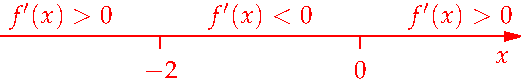
\includegraphics[scale=0.9]{mvt-ex3}
  	\end{center}
  \end{minipage}\begin{minipage}[t]{0.4\linewidth}\vspace{0pt}
  \flushright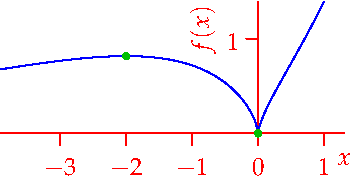
\includegraphics{mvt-ex2}
  \end{minipage}\smallbreak	
	By the 1\st\ derivative test, $f$ has a maximum at $x=-2$ and a minimum at $x=0$.
\end{enumerate}
\end{examples}

We finish this section by tying together the mean and intermediate value theorems.

\begin{thm}{IVT for Derivatives}{intvalderiv}
Suppose $f$ is differentiable on an interval $I$ containing $a<b$, and that $L$ lies between $f'(a)$ and $f'(b)$. Then $\exists\xi\in(a,b)$ such that $f'(\xi)=L$.
\end{thm}

If $f'(x)$ is \emph{continuous,} this is just the intermediate value theorem applied to $f'$. A full proof is left to the exercises; surprisingly, continuity is \emph{not} required\ldots

\goodbreak


% \begin{proof}
% Define $g:I\to\R$ by $g(x)=f(x)-Lx$ and let $\xi\in[a,b]$ be such that\footnote{$g$ differentiable $\implies g$ continuous on the bounded interval $[a,b]$. The extreme value theorem says $g$ is bounded and attains its bounds.}
% \[g(\xi)=\min\{g(x):x\in[a,b]\}\]
% If $\xi\in(a,b)$, Lemma \ref{lemm:rolle} says that $g'(\xi)=0\implies f'(\xi)=L$.\\[5pt]
% To complete the proof, we need to prove that $\xi\neq a$ or $b$. WLOG, assume that $f'(a)<f'(b)$. Then
% \[g'(a)=f'(a)-L<0<f'(b)-L=g'(b)\]
% In particular,
% \[\lim_{x\to a^+}\frac{g(x)-g(a)}{x-a}=g'(a)<0 \implies \exists \delta>0\text{ such that }a<x<a+\delta\implies g(x)<g(a)\]
% whence $g(a)$ is not the minimum value of $g$ on $[a,b]$. That $g(b)$ is not the minimum is similar.
% \end{proof}

% The classic example of a differentiable function with discontinuous derivative is
% \[f(x)=\begin{cases}
% x^2\sin(1/x)&x\neq 0\\
% 0&x=0
% \end{cases} \implies f'(x)=\begin{cases}
% 2x\sin(1/x)-\cos(1/x)&x\neq 0\\
% 0&x=0
% \end{cases}\]
% We leave the analysis of this to the homework.

% The derivative is discontinuous at $x=0$. We can still apply the theorem however. For instance, given $n\in\N$, let $a=0$ and $b=\frac 1{2\pi n}$ so that $f'(a)=0>f'(b)=-1$. If $L$ is any number in this interval, the theorem says
% \[\exists \xi_n\in\left(0,\frac 1{2\pi n}\right)\text{ such that }f'(x_n)=L\]
% With a little thinking, this says that the set of all possible limits $\lim\limits_{n\to\infty}f(x_n)$ taken over all sequences $x_n\to 0$ is in fact the interval $[-1,1]$!\goodbreak


% \begin{cor}{}{incdec}
% Suppose $f$ is differentiable on an interval and that $f'(x)\neq 0$. Then $f$ is either strictly increasing or strictly decreasing.
% \end{cor}
% 
% The proof is an easy exercise.

% \begin{proof}
% Suppose $a,b\in I$, that $f'(a)<0<f'(b)$. Then $\exists\xi$ such that $f'(\xi)=0$. Contradiction. it follows that 
% \end{proof}

\begin{exercises}
\exstart Determine whether the conclusion of the mean value theorem holds for each function on the given interval. If so, find a suitable point $\xi$. If not, state which hypothesis fails.
\begin{enumerate}\setcounter{enumi}{1}\itemsep0pt
  \item[]\begin{enumerate}
    \item $x^2$ on $[-1,2]$\qquad\qquad (b)\space\space $\sin x$ on $[0,\pi]$\qquad\qquad (c)\space\space $\nm x$ on $[-1,2]$
    \item[(d)] $1/x$ on $[-1,1]$\qquad\qquad (e)\space\space $1/x$ on $[1,3]$
  \end{enumerate}
  
  \item Suppose $f$ and $g$ are differentiable on an open interval $I$, that $a<b$ and $f(a)=f(b)=0$. By considering $h(x)=f(x)e^{g(x)}$, prove that $f'(\xi)+f(\xi)g'(\xi)=0$ for some $\xi\in (a,b)$.
  
  \item Use the Mean Value Theorem to prove the following:\vspace{-5pt}
  \begin{enumerate}
    \item $x<\tan x$ for all $x\in(0,\pi/2)$.
    \item $\frac{x}{\sin x}$ is a strictly increasing function on $(0,\pi/2)$.
    \item $x\le\frac{\pi}2\sin x$ for all $x\in[0,\pi/2]$.
  \end{enumerate}
  
  \item Suppose that $\nm{f(x)-f(y)}\le (x-y)^2$ for all $x,y\in\R$. Prove that $f$ is a constant function.  
  
	\item\begin{enumerate}
	  \item Prove that $f'>0$ on an interval $I\implies f$ is \emph{strictly} increasing on $I$.
	  \item Show that the converse of part (a) is \emph{false.}
  	\item Carefully prove the first derivative test (Corollary \ref{cor:1stderivtest}).
	\end{enumerate}
% 	but the converse does not. For example, $f:x\mapsto x^3$ is strictly increasing on $\R$ with derivative $f'(x)=3x^2\ge 0$: clearly $f'(0)=0$.
	
  \item\label{exs:fincdec} If $f$ is differentiable on an interval $I$ such that $f'(x)\neq 0$ for all $x\in I$, use the intermediate value theorem for derivatives to prove that $f$ is either strictly increasing or strictly decreasing.
  
  \item We prove the intermediate value theorem for derivatives. Let $f,a,b$ and $L$ be as in the Theorem, define $g:I\to\R$ by $g(x)=f(x)-Lx$, and let $\xi\in[a,b]$ be such that
	\[g(\xi)=\min\{g(x):x\in[a,b]\}\]
	\begin{enumerate}
	  \item Why can we be sure that $\xi$ exists? If $\xi\in(a,b)$, explain why $f'(\xi)=L$.
		\item Now assume WLOG that $f'(a)<f'(b)$. Prove that $g'(a)<0<g'(b)$. By considering $\lim\limits_{x\to a^+}\frac{g(x)-g(a)}{x-a}$, show that $\exists x>a$ for which $g(x)<g(a)$. Hence complete the proof.
	\end{enumerate}
  
  \item Suppose $f'$ exists on $(a,b)$, and is continuous except for a discontinuity at $c\in(a,b)$.
  \begin{enumerate}
    \item Obtain a contradiction if $\lim\limits_{x\to c^+}f'(x)=L<f'(c)$. Hence argue that $f'$ cannot have a \emph{removable} or a \emph{jump} discontinuity at $x=c$.\\
    (\emph{Hint: let $\epsilon=\frac{f'(c)-L}2$ in the definition of limit then apply IVT for derivatives})
    \item Similarly, obtain a contradiction if \smash[b]{$\lim\limits_{x\to c^+}f'(x)=\infty$} and conclude that $f'$ cannot have an \emph{infinite} discontinuity at $x=c$.
  	\item It remains to see that $f'$ can have an essential discontinuity. Recall (Exercise \hyperref[exs:diffdiscont]{\ref*{sec:derivproperties}.\ref*{exs:diffdiscont}}) that
		\[f:\R\to\R:x\mapsto \begin{cases}
		x^2\sin(1/x)&x\neq 0\\
		0&x=0
		\end{cases}\]
		is differentiable on $\R$, but has discontinuous derivative at $x=0$.
		\begin{enumerate}
  		\item By considering $x_n=\frac 1{2n\pi}$ and $y_n=\frac 1{(2n+1)\pi}$, show that $f'$ has an essential discontinuity at $x=0$.
  		\item Prove that if $s_n\to 0$ and $f'(s_n)$ converges to some $M$, then $M\in[-1,1]$.
			\item Use IVT for derivatives to show that for any $L\in[-1,1]$, $\exists (t_n)\subseteq\R\setminus\{0\}$ such that $\lim\limits_{n\to \infty}f'(t_n)=L$. 
		\end{enumerate}
  \end{enumerate}
\end{enumerate}
\end{exercises}

\goodbreak

\subsection{L'Hôpital's Rule}\label{sec:lhopital}

We are often forced to consider limits known as \emph{indeterminate forms,} which do not yield easily to the standard limits laws. For example, it is tempting to try to write
\[\lim_{x\to 0}\frac{\sin 2x}{e^{3x}-1}=\frac{\lim\limits_{x\to 0}\sin 2x}{\lim\limits_{x\to 0}e^{3x}-1} =\frac 00\tag{$\ast$}\]
This is an incorrect application of the limit laws since the resulting quotient has no meaning.

\begin{defn}{}{indetform}
An \emph{indeterminate form} is a limit where a naïve application of the limit laws results in a meaningless expression: the primary types are $\frac 00$, $\frac\infty\infty$, $\infty-\infty$, $0\cdot\infty$, $0^0$, $0^\infty$, and $1^\infty$.
\end{defn}

\begin{examples}{}{}
\exstart $\lim\limits_{x\to 7^+}(x-7)^\frac 1{x-7}$ is an indeterminate form of type $0^\infty$.
\begin{enumerate}\setcounter{enumi}{1}
  \item The above indeterminate form $(\ast)$ may be evaluated using the definition of the derivative
	\[\lim_{x\to 0}\frac{\sin 2x}{e^{3x}-1}= \lim_{x\to 0}\frac{\sin 2x-0}{x-0}\frac{x-0}{e^{3x}-1} =\left(\diffat x{x=0}\sin 2x\right) \left(\diffat x{x=0}e^{3x}\right)^{-1} =\frac 23\]
	By considering $\lim\limits_{x\to 0}\frac{3a\sin 2x}{2(e^{3x}-1)}$, we see that an indeterminate form of type $\frac 00$ can take \emph{any value} $a$!
\end{enumerate}
\end{examples}

This approach generalizes: if $f(a)=0=g(a)$, we obtain the simplest version of l'Hôpital's rule;
\[\tcbhighmath{\lim_{x\to a}\frac{f(x)}{g(x)}=\lim_{x\to a}\frac{f(x)-f(a)}{x-a}\cdot \frac{x-a}{g(x)-g(a)} =\frac{f'(a)}{g'(a)}}\]
This obviously isn't rigorous. Our goal is to make it so and to extend to the following situations:
\begin{itemize}
  \item Limits where $a=\pm\infty$.
  \item When the RHS cannot be cleanly evaluated: for instance $g'(a)=0$ or if the original limit is $\pm\infty$.
\end{itemize}

Covering all cases makes the proof an absolute behemoth! Because of this, and because such limits can often be evaluated more instructively using elementary methods, the rule is often discouraged in Freshman calculus. To prepare for the upcoming monster, we first  generalize the MVT.

\begin{lemm}{Extended Mean Value Theorem}{extmvt}
Fix $a<b$, suppose $f,g$ are continuous on $[a,b]$ and differentiable on $(a,b)$. Then there exists $\xi\in(a,b)$ such that
\[\big(f(b)-f(a)\big)g'(\xi)=\big(g(b)-g(a)\big)f'(\xi)\] 
\end{lemm}

\begin{proof}
Simply apply the standard mean value theorem (really \hyperref[lemm:rolle]{Rolle's Theorem}) to
\[h(t)=(f(b)-f(a))g(t)-(g(b)-g(a))f(t)\]
which satisfies $h(a)=h(b)$.
\end{proof}\goodbreak

\begin{thm}{l'Hôpital's rule}{}
Let $a\in\R\cup\{\pm\infty\}$ and suppose functions $f$ and $g$ satisfy:
\begin{enumerate}%\itemsep0pt
  \item $\displaystyle\lim\limits_{x\to a}\frac{f'(x)}{g'(x)}=L$ for some $L\in\R\cup\{\pm\infty\}$
  \item (a)\space\space $\displaystyle\lim\limits_{x\to a}f(x)=\lim\limits_{x\to a} g(x)=0$,\quad or\quad (b)\space\space $\displaystyle\lim\limits_{x\to a}g(x)=\infty$\space\space (no condition on $f$)
\end{enumerate}
Then $\displaystyle\lim\limits_{x\to a}\frac{f(x)}{g(x)}=L$. The same result holds for one-sided limits.
\end{thm}

\vfil

\begin{examples}{}{lhopital}
\exstart If $f(x)=e^{4x}$ and $g(x)=21x-17$, then
  \[\lim_{x\to\infty}\frac{f'(x)}{g'(x)}=\lim_{x\to\infty}\frac{4e^{4x}}{21}=\infty\implies \lim_{x\to\infty}\frac{e^{4x}}{21x-17}=\infty\]
  This is an example of type $\frac\infty\infty$.
\begin{enumerate}\setcounter{enumi}{1}
  \item For an example of type $\frac 00$, consider $f(x)=x^2-9$ and $g(x)=\ln(4-x)$:
  \[\lim_{x\to 3^-}\frac{f'(x)}{g'(x)} = \lim_{x\to 3^-}\frac{2x}{-1/(4-x)} = \lim_{x\to 3^-}2x(x-4)=-6\implies \lim_{x\to 3^-}\frac{x^2-9}{\ln(4-x)}=-6\]
  \item One can apply the rule repeatedly: for example
  \[\lim_{x\to 0}\frac{e^{4x}-1-4x}{x^2}=\lim_{x\to 0}\frac{4e^{4x}-4}{2x} =\lim_{x\to 0}\frac{16e^{4x}}{2}=8\]
  There is an abuse of protocol here, since the existence of the first limit is dependent on the last. The approach is acceptable, though you should understand why it is an abuse. Indeed\ldots
  \item\label{ex:lhopitalproblem1} It is important that the limit $\lim\frac{f'}{g'}$ be seen to exist \emph{before} applying l'Hôpital's rule! Consider $f(x)=x+\cos x$ and $g(x)=x$: certainly $\lim\limits_{x\to\infty}\frac{f(x)}{g(x)}$ has type $\frac\infty\infty$, however
  \[\lim\limits_{x\to\infty}\frac{f'(x)}{g'(x)}=\lim\limits_{x\to\infty}1-\sin x\]
  does not exist! In this case the rule is unnecessary, since
  \[\frac{f(x)}{g(x)}=1+\frac{\cos x}x\xrightarrow[x\to\infty]{} 1\]
  by the squeeze theorem.
 	\item Finally, a short example to explain why l'Hôpital's rule is often prohibited in Freshman calculus. Consider the calculation:
 	\[\lim_{x\to 0}\frac{\sin x}x=\lim_{x\to 0}\frac{\cos x}{1}=1\]
 	This appears to be a legitimate application of the rule. However, recall (Exercise \hyperref[ex:trigdiff]{\ref*{sec:derivproperties}.\ref*{ex:trigdiff}}) that one purpose of this limit is to demonstrate that $\diff x\sin x=\cos x$; to use this fact to calculate the limit on which it depends is the very definition of circular logic!
\end{enumerate}
\end{examples}

\boldsubsubsection{Other Indeterminate Forms}

The remaining indeterminate forms listed in Definition \ref{defn:indetform} may be modified so that l'Hôpital's rule applies. Since you've likely seen several such examples in elementary calculus, we give just a couple.


\begin{examples}{}{}
\exstart An indeterminate form of type $\infty-\infty$ is transformed to one of type $\frac 00$ before applying the rule (twice):
  \begin{align*}
  	\lim\limits_{x\to 0^+}\frac 1{e^x-1}-\frac 1x&=\lim\limits_{x\to 0^+}\frac{x+1-e^x}{x(e^x-1)} \tag{type $\frac 00$}\\
  	&=\lim\limits_{x\to 0^+}\frac{1-e^x}{e^x-1+xe^x} \tag{still type $\frac 00$}\\
  	&=\lim\limits_{x\to 0^+}\frac{-e^x}{2e^x+xe^x} =-\frac 12
  \end{align*}
\begin{enumerate}\setcounter{enumi}{1}
 	\item For an indeterminate form of type $1^\infty$, we use the log laws \& the continuity of the exponential:
 	\begin{align*}
 	\lim_{x\to 0^+} (1+\sin x)^{1/x}&=\exp\left(\lim_{x\to 0^+} \frac 1x\ln(1+\sin x)\right) \tag{type $\frac 00$}\\
 	&=\exp\left(\lim_{x\to 0^+} \frac{\cos x}{1+\sin x}\right)\\
 	&=e^1=e
 	\end{align*}
 	\end{enumerate}
\end{examples}

\boldsubsection{Proving l'Hôpital's Rule}

The complete argument is very long; if you do nothing else, read the following proof of the simplest case. Everything else is a modification.

\begin{proof}[Proof (type $\frac 00$ with right limits)]
We prove first for \emph{right-limits} $x\to a^+$. First observe that condition 1.\ forces the existence of an interval $(a,b)$ on which $f,g$ are differentiable and $g'(x)\neq 0$.\smallbreak
Assume we have a form of type $\frac 00$ (case 2.\,(a)) and assume additionally that $a$ and $L$ are finite. Everything follows from the definition of limit (condition 1.) and Lemma \ref{lemm:extmvt}:
\begin{gather*}
\textcolor{Green}{\text{Given $\epsilon>0$, }} \textcolor{blue}{\exists\delta\in(0,b-a)\text{ such that }a<\xi<a+\delta}\implies \textcolor{Green}{\nm{\frac{f'(\xi)}{g'(\xi)}-L}<\frac\epsilon 2}\tag{$\ast$}\\
a<y<x<a+\delta\implies \exists\xi\in(y,x)\text{ such that }\frac{f(x)-f(y)}{g(x)-g(y)}=\frac{f'(\xi)}{g'(\xi)} \tag{$\dag$}
\end{gather*}
Since $g'\neq 0$, the usual mean value theorem says we never divide by zero in $(\dag)$:
\[\exists c\in(y,x)\text{ such that } g(x)-g(y)=g'(c)(x-y)\neq 0\]
Observe that $\nm{\frac{f(x)-f(y)}{g(x)-g(y)}-L}=\nm{\frac{f'(\xi)}{g'(\xi)}-L}<\frac\epsilon 2$, let $y\to a^+$ and use 2.\,(a)\ to see that
\[\forall x\in(a,a+\delta),\quad \nm{\frac{f(x)}{g(x)}-L}\le\frac\epsilon 2<\epsilon\]
which is the required result.
\end{proof}

We now describe some modifications.
\begin{description}\itemsep1pt
	\item[\normalfont\emph{If $a=-\infty$}:] Replace the blue part of ($\ast$) as follows:
	\[\textcolor{Green}{\text{Given $\epsilon>0$, }} \textcolor{blue}{\exists m\le b\text{ such that }\xi<m}\implies \textcolor{Green}{\smash[t]{\nm{\frac{f'(\xi)}{g'(\xi)}-L}<\frac\epsilon 2}}\]
	The rest of the proof goes through after replacing $a$ with $-\infty$ and $a+\delta$ with $m$.
	\item[\normalfont\emph{If $L=\infty$}:] Replace the green parts of ($\ast$) with \textcolor{Green}{Given $M>0$} and $\textcolor{Green}{\frac{f'(\xi)}{g'(\xi)}>2M}$. Fixing the rest of the proof is again straightforward.
	\item[\normalfont\emph{If $L=-\infty$}:] Replace the green parts of ($\ast$) with \textcolor{Green}{Given $M>0$} and $\textcolor{Green}{\frac{f'(\xi)}{g'(\xi)}<-2M}$.
	\item[\normalfont\emph{Left-limits}:] If $f,g$ are differentiable on $(c,a)$, then the blue part may be replaced with either:
	\begin{itemize}
	  \item ($a$ finite)\quad\textcolor{blue}{$\exists\delta\in(0,a-c)\text{ such that }a-\delta<\xi<a$}
	  \item ($a=\infty$)\quad $\textcolor{blue}{\exists m\ge c\text{ such that }\xi>m}$
	\end{itemize} 
\end{description}
The blue and green parts of ($\ast$) can be replaced independently. This completes the proof for all indeterminate forms of type $\frac 00$.

\begin{proof}[Proof (case 2.\,(b) when $\lim g(x)=\infty$)]
This requires a little more modification.\footnotemark Since $g'\neq 0$, and $\lim_{x\to a^+}g(x)=\infty$, Exercise \hyperref[exs:fincdec]{\ref*{sec:mvt}.\ref*{exs:fincdec}} says that $g$ is \emph{strictly decreasing} on $(a,b)$. By replacing $b$ by some $\tilde b\in(a,b)$, if necessary, we may assume that
\[a<y<x<b\implies 0<g(x)<g(y)\tag{\ddag}\]
Assume $a$ and $L$ are finite, and obtain $(\ast)$ and $(\dag)$ as before. Let $x\in(a,a+\delta)$ be fixed and multiply ($\dag$) by $\frac{g(y)-g(x)}{g(y)}$ (this is \emph{positive} by ($\ddag$)): a little algebra and the triangle inequality tell us that 
\begin{align*}
a<y<x \implies& \frac{f(y)}{g(y)} =\frac{f'(\xi)}{g'(\xi)}+\frac{f(x)}{g(y)}- \frac{g(x)}{g(y)}\cdot\frac{f'(\xi)}{g'(\xi)}\\
\implies& \nm{\frac{f(y)}{g(y)}-L}\le \nm{\frac{f'(\xi)}{g'(\xi)}-L} +\frac 1{g(y)}\left(\nm{f(x)}+\nm{g(x)}\left(L+\frac\epsilon 2\right)\right)
\end{align*}
Since $\lim\limits_{y\to a^+}g(y)=\infty$ and $x$ is fixed, we see that there exists $\eta\le x-a<\delta$ such that
\[y\in(a,a+\eta)\implies \frac 1{g(y)}\left(\nm{f(x)}+\nm{g(x)}\left(L+\frac\epsilon 2\right)\right) <\frac\epsilon 2\]
Finally combine with $(\ast)$: given $\epsilon>0,\exists \eta>0$ such that $y\in(a,a+\eta)\implies \nm{\frac{f(y)}{g(y)}-L}<\epsilon$.\\
The same modifications listed previously complete the proof.
\end{proof}

\footnotetext{\emph{Forms of type $\frac\infty\infty$?}\quad Instead of assumption 2.\,(b), why not simply assume $\lim f=\lim g=\infty$ and write $\frac fg=\frac{1/g}{1/f}$ to obtain a form of type $\frac 00$? The problem is that the derivative of the `new' denominator $\diff x\frac 1f=\frac{-f'}{f^2}$ need not be non-zero on any interval $(a,b)$ and so condition 1.\ need not hold. We could modify this, but it would make for a weaker theorem. Example \hyperref[ex:lhopitalproblem1]{\ref*{ex:lhopital}.\ref*{ex:lhopitalproblem1}} illustrates this: $f'(x)=1+\sin x$ has zeros on any unbounded interval.\par
\emph{After} the 2.\,(b) case is proved and we know that $\lim\frac fg=L$, it is then clear that $\lim f$ must also be infinite (unless $L=0$ in which case $\lim f$ could be anything and need not exist). This situation therefore really does deal with forms of type $\frac\infty\infty$.}




\begin{exercises}
\exstart Evaluate the following limits, if they exist:\vspace{-5pt}
\begin{enumerate}\setcounter{enumi}{1}
  \item[]\renewcommand{\arraystretch}{1.5}
  \begin{tabular}{r@{\ \ }l@{\qquad}r@{\ \ }l}
  (a)
  &
  $\displaystyle\lim_{x\to 0}\frac{x^3}{\sin x-x}$
  &
  (b)
  &
  $\displaystyle\lim_{x\to {\frac\pi 2}^-}\tan x-\frac 2{\pi-2x}$
  \\
  (c)
  &
  $\displaystyle\lim_{x\to 0}(\cos x)^{1/x^2}$
	&
	(d)
	&
	$\displaystyle\lim_{x\to 0}(1+2x)^{1/x}$
	\\
	(e)
	&
	$\displaystyle\lim_{x\to \infty}(e^x+x)^{1/x}$
  &
  \end{tabular}
  	
	\item Let $f$ be differentiable on $(c,\infty)$ and suppose that $\lim\limits_{x\to\infty}[f(x)+f'(x)]=L$ is finite.
	\begin{enumerate}
	  \item Prove that $\lim\limits_{x\to\infty}f(x)=L$ and that $\lim\limits_{x\to\infty}f'(x)=0$.\\
		(\emph{Hint: write $f(x)=\frac{f(x)e^x}{e^x}$})
		\item Does anything change if $L$ exists and is \emph{infinite}?
	\end{enumerate}
	
	\item\label{exs:pnexplimit} If $p_n(x)$ is a polynomial of degree $n$, use induction to prove that $\lim\limits_{x\to\infty}p_n(x)e^{-x}=0$
	
	\item Let $f(x)=x+\sin x\cos x$, \ $g(x)=e^{\sin x}f(x)$ and $h(x)=\dfrac{2\cos x}{e^{\sin x}(f(x)+2\cos x)}$
	\begin{enumerate}
	  \item Prove that $\lim\limits_{x\to\infty}f(x)=\infty=\lim\limits_{x\to\infty}g(x)$ but that $\lim\limits_{x\to\infty}\frac{f(x)}{g(x)}$ does not exist.
	  \item If $\cos x\neq 0$, and $x$ is large, show that $\frac{f'(x)}{g'(x)}=h(x)$.
	  \item Prove that $\lim\limits_{x\to\infty}h(x)=0$. Explain why this does not contradict part (a)!
	\end{enumerate}
\end{enumerate}
\end{exercises}
\clearpage

\subsection{Taylor's Theorem}

A primary goal of power series is the approximation of functions. As such, there are two natural questions to ask of a given function $f$:\vspace{-8pt}
\begin{enumerate}\itemsep0pt
  \item\label{taylormotiv} Given $c\in\dom(f)$, is there a series $\sum a_n(x-c)^n$ which equals $f(x)$ on an interval containing $c$?
  \item If we take the first $n$ terms of such a series, how accurate is this polynomial approximation?
\end{enumerate}

\begin{example}{}{}
Recall the geometric series\smallbreak
\begin{minipage}[t]{0.59\linewidth}\vspace{-12pt}
\[\textcolor{blue}{f(x)=\frac 1{1-x}}=\sum_{n=0}^\infty x^n\text{ whenever }-1<x<1\]
The polynomial approximation
\[p_n(x)=\sum_{k=0}^nx^k=1+x+\cdots+x^n =\frac{1-x^{n+1}}{1-x}\]
has error
\[R_n(x)=f(x)-p_n(x)=\frac{x^{n+1}}{1-x}\]
\end{minipage}
\begin{minipage}[t]{0.4\linewidth}\vspace{-20pt}
\flushright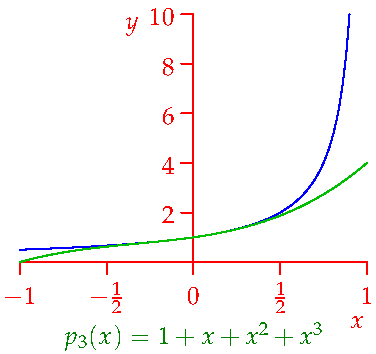
\includegraphics{taylor-remainder}
\end{minipage}\medbreak
If $x$ is close to 0, this is likely very small; for instance if $x\in\left[-\frac 12,\frac 12\right]$, then
\[\nm{R_n(x)}\le\frac 1{1-\frac 12}\left(\frac 12\right)^{n+1}=2^{-n}\]
However, when $x$ is close to 1, the error is unbounded!
\end{example}

The behavior in the Example occurs in general: the truncated polynomial approximations are better near the center of the series. To see this, we first need to consider higher-order derivatives.

\begin{defn}{}{}
We write $f''$ for the \emph{second derivative} of $f$, namely the derivative of its derivative
\[f''(a)=\lim_{x\to a}\frac{f'(x)-f'(a)}{x-a}\]
The existence of $f''(a)$ presupposes that $f'$ exists on an (open) interval containing $a$. We can similarly consider third, fourth, and higher-order derivatives. As a function, the $n\th$ derivative is written
\[f^{(n)}(x)=\diff[^nf]{x^n}\]
By convention, the \emph{zeroth derivative} is the function itself $f^{(0)}(x)=f(x)$. We say that $f$ is \emph{$n$ times differentiable} at $a$ if $f^{(n)}(a)$ exists, and \emph{infinitely differentiable} (or \emph{smooth}) if derivatives of all orders exist.
\end{defn}

\begin{example}{}{}
$f(x)=x^2\nm x$ is twice differentiable, with $f''(x)=6\nm x$. It is smooth everywhere except at $x=0$, where third (and higher-order) derivatives do not exist.
\end{example}

\goodbreak

\begin{defn}{}{}
Suppose $f$ is $n$ times differentiable at $x=c$. The \emph{$n\th$ Taylor polynomial} $p_n$ of $f$ centered at $c$ is
\[p_n(x):=\sum_{k=0}^n\frac{f^{(k)}(c)}{k!}(x-c)^k =f(c)+f'(c)(x-c)+\frac{f''(c)}2(x-c)^2+\cdots+\frac{f^{(n)}(c)}{n!}(x-c)^n\]
The \emph{remainder} $R_n(x)$ is the error in the polynomial approximation
\[R_n(x)=f(x)-p_n(x)=f(x)-\sum_{j=0}^{n}\frac{f^{(k)}(c)}{k!}(x-c)^k\]
If $f$ is infinitely differentiable at $x=c$, then its \emph{Taylor series} centered at $x=c$ is the power series
\[\rT f(x)=\sum_{n=0}^\infty\frac{f^{(n)}(c)}{n!}(x-c)^n\]
When $c=0$ this is known as a \emph{Maclaurin series.}\footnotemark
\end{defn}

\footnotetext{Named for Englishman Brook Taylor (1685--1731) and Scotsman Colin Maclaurin (1698--1746). Taylor's general method expanded on examples discovered by James Gregory and Issac Newton in the mid-to-late 1600's.}

For simplicity we'll most often work with Maclaurin series, with general cases hopefully being clear.

\begin{examples}{}{basictaylor}
\exstart If $f(x)=e^{3x}$, then $f^{(n)}(x)=3^ne^x$, from which the Maclaurin series is\vspace{-18pt}
\begin{enumerate}\setcounter{enumi}{1}
  \item[]\[\rT f(x)=\sum_{n=0}^\infty\frac{3^n}{n!}x^n\]
  \item If $g(x)=\sin 7x$, then the sequence of derivatives is
  \[7\cos 7x,\ \ -7^2\sin 7x,\ \ -7^3\cos 7x,\ \ 7^4\sin 7x,\ \ 7^5\cos 7x,\ \ -7^6\sin 7x,\ldots\]
	At $x=0$, every even derivative is zero, while the odd derivatives alternate in sign; the Maclaurin series is easily seen to be
  \[\rT g(x)=\sum_{n=0}^\infty\frac{(-1)^n7^{2n+1}}{(2n+1)!}x^{2n+1}\]
  \item\label{ex:basictaylor3} If $h(x)=\sqrt x$, then $h'(x)=\frac 12x^{-1/2}$, $h''(x)=\frac{-1}{2^2}x^{-3/2}$, and $h'''(x)=\frac{3}{2^3}x^{-5/2}$, from which the third Taylor polynomial centered at $c=1$ is
  \begin{align*}
  p_2(x)&=h(1)+h'(1)(x-1)+\frac{h''(1)}{2}(x-1)^2+\frac{h'''(1)}{6}(x-1)^3\\
  &=1+\frac 12(x-1)-\frac 18(x-1)^2+\frac 1{16}(x-1)^3
  \end{align*}
\end{enumerate}
\end{examples}

Rather than compute more examples, we develop a little theory that makes verifying Taylor series much easier.
\goodbreak


	
\boldsubsubsection{Differentiation of Taylor Polynomials and Series}
	
Suppose $P(x)=\sum a_jx^j$ is a power series with radius of convergence $R>0$. As we discovered previously, this is differentiable term-by-term on $(-R,R)$. Indeed
\begin{gather*}
%P(0)=a_0\\
P'(x)=\sum_{j=1}^\infty a_jjx^{j-1} \implies P'(0)=a_1\\
P''(x)=\sum_{j=2}^\infty a_jj(j-1)x^{j-2} \implies P''(0)=2a_2\\
P'''(x)=\sum_{j=3}^\infty a_jj(j-1)(j-2)x^{j-3} \implies P'''(0)=3!a_3\\[-8pt]
\quad\vdots\\[-3pt]
P^{(k)}(x)=\sum_{j=k}^\infty a_jj(j-1)\cdots(j-k+1)x^{j-k}=\sum_{j=k}^\infty\frac{j!a_j}{(j-k)!}x^{j-k} \implies P^{(k)}(0)=k!a_k
\end{gather*}
Otherwise said, $P$ is its own Maclaurin series! The same discussion holds for polynomials: indeed if $P(x)=a_0+a_1x+\cdots+a_nx^n$ is a polynomial, then for all $k\le n$,
\[P^{(k)}(0)=f^{(k)}(0)\iff a_k=\frac{f^{(k)}(0)}{k!}\]
If this holds for \emph{all} $k\le n$, then $P$ must be the Taylor polynomial of $f$! With a little modification, we've proved the following:

\begin{thm}{}{taylorlem}
\exstart If $f(x)=\smash[b]{\sum\limits_{n=0}^\infty} a_n(x-c)^n$ on a neighborhood of $c$, then $\smash[b]{\sum\limits_{n=0}^\infty} a_n(x-c)^n$ is the Taylor series of $f$.
\begin{enumerate}\setcounter{enumi}{1}
	\item The $n\th$ Taylor polynomial of $f$ centered at $x=c$ is the unique polynomial $p_n$ of degree $\le n$ whose value and first $n$ derivatives agree with those of $f$ at $x=c$: that is
	\[\forall k\le n,\ \ \smash[t]{p_n^{(k)}(c)=f^{(k)}(c)}\]
\end{enumerate}
\end{thm}

This answers our first \hyperref[taylormotiv]{motivating question:} a function can equal at most one power series with a given center. The second question requires a careful study of the \emph{remainder}: we'll do this shortly.

\begin{examples}{Common Maclaurin Series}{taylorexs}
These should be familiar from elementary calculus. Each of these functions equals the given series by our previous discussion of power series: by the Theorem, each series is therefore the Maclaurin series of the given function with no requirement to calculate directly!
\[\def\arraystretch{2}
\begin{array}{ll@{\qquad\qquad\qquad}ll}
\displaystyle e^x=\sum_{n=0}^\infty\frac{x^n}{n!} & x\in\R
&\displaystyle\frac 1{1-x}=\sum_{n=0}^\infty x^n & x\in(-1,1)\\
\displaystyle\sin x=\sum_{n=0}^\infty\frac{(-1)^n}{(2n+1)!}x^{2n+1} & x\in\R
&\displaystyle\ln(1+x)=\sum_{n=1}^\infty \frac{(-1)^{n+1}}nx^n & x\in (-1,1]\\
\displaystyle\cos x=\sum_{n=0}^\infty\frac{(-1)^n}{(2n)!}x^{2n} & x\in\R
&\displaystyle\tan^{-1}x=\sum_{n=0}^\infty \frac{(-1)^n}{2n+1}x^{2n+1} & x\in[-1,1]
\end{array}
\]
\end{examples}

\goodbreak

% 
% \[\def\arraystretch{2}
% \begin{array}{c|c|c}
% \text{Function $f(x)$} & \text{Maclaurin Series $\rT f(x)$} & \text{Interval of convergence}\\\hline
% e^x & \displaystyle\sum_{n=0}^\infty\frac{x^n}{n!} & (-\infty,\infty)\\
% \sin x & \displaystyle\sum_{n=0}^\infty\frac{(-1)^n}{(2n+1)!}x^{2n+1} & (-\infty,\infty)\\
% \cos x & \displaystyle\sum_{n=0}^\infty\frac{(-1)^n}{(2n)!}x^{2n} & (-\infty,\infty)\\
% \dfrac 1{1-x} & \displaystyle\sum_{n=0}^\infty x^n & (-1,1)\\
% \ln(1+x) & \displaystyle\sum_{n=1}^\infty \frac{(-1)^{n+1}}nx^n & (-1,1]\\
% \tan^{-1}x & \displaystyle\sum_{n=0}^\infty \frac{(-1)^n}{2n+1}x^{2n+1} & [-1,1]
% \end{array}\]

\begin{examples}{Modifying Maclaurin Series}{modmaclaurin}
By substituting for $x$ in a common series, we quickly obtain new ones.
\begin{enumerate}
  \item Substitute $x\mapsto 7x$ in the Maclaurin series for $\sin x$, to recover our earlier example
 	\[\sin 7x=\sum_{n=0}^\infty\frac{(-1)^n7^{2n+1}}{(2n+1)!}x^{2n+1},\quad x\in \R\]
	Note how this requires almost no calculation: since the function equals a series, the Theorem says we have the Maclaurin series for $\sin 7x$!
	
	\item Substitute $x\mapsto x^2$ in the Maclaurin series for $e^x$ to obtain
  \[e^{x^2}=\exp(x^2)=\sum_{n=0}^\infty \frac{1}{n!}x^{2n},\quad x\in\R\]
  This would be disgusting to verify directly, given the difficulty of repeatedly differentiating $e^{x^2}$.
  
  \item We find the Taylor series for $f(x)=\frac 1{5-x}$ centered at $x=2$:
  \[f(x)=\frac 1{3+2-x} =\frac 1{3(1-\frac{2-x}3)} =\frac 13\sum_{n=0}^\infty\left(\frac{2-x}3\right)^n\]
  which is valid whenever $-1<\frac{2-x}3<1\iff -1<x<5$.
  
  \item Fix $c\in\R$ and observe that, for all $x\in\R$,
  \[e^x=e^{c+x-c}=e^ce^{x-c}=\sum_{n=0}^\infty \frac{e^c}{n!}(x-c)^n\]
  We conclude that the series is the Taylor series of $e^x$ centered at $x=c$. Of course this is easily verified using the definition, since $\diffat[^n]{x^n}{x=c}e^x=e^c$.
  
  \item Combining the Theorem with the multiple-angle formula, we obtain the Taylor series for $\sin x$ centered at $x=c$:
  \begin{align*}
  \sin x&=\sin(c+x-c)=\sin c\cos(x-c)+\cos x\sin(x-c)\\
  &=\sum_{n=0}^\infty\frac{(-1)^n\sin c}{(2n)!}(x-c)^{2n} +\sum_{n=0}^\infty\frac{(-1)^n\cos c}{(2n+1)!}(x-c)^{2n+1}
  \end{align*}
\end{enumerate}
\end{examples}


\begin{defn}{}{}
A function is \emph{analytic} on a domain if for each $c$ there exists a neighborhood of $c$ on which the function equals its Taylor series centered at $c$.
\end{defn} 
	
All the examples we've so far seen are analytic on their domains; indeed the last two of Examples \ref{ex:modmaclaurin} \emph{prove} this for the exponential and sine functions. Every analytic function is automatically smooth (infinitely differentiable), however the converse is \emph{false} in that not every smooth function is analytic (see Exercise \ref{exs:macnoteq}). Analyticity is of greater importance in complex analysis where it is seen to be equivalent to complex-differentiability.

\boldsubsubsection{Accuracy of Taylor Approximations}

Our final goal is to estimate the accuracy of a Taylor polynomial as an approximation to its generating function. Otherwise said, we want to estimate the size of the remainder $R_n(x)=f(x)-p_n(x)$.

\begin{thm}{Taylor's Theorem: Lagrange's form}{taylor}
Suppose $f$ is $n+1$ times differentiable on an open interval $I$ containing $c$ and let $x\in I\setminus\{c\}$. Then there exists some $\xi$ between $c$ and $x$ for which the remainder centered at $c$ satisfies
\[R_n(x)=\frac{f^{(n+1)}(\xi)}{(n+1)!}(x-c)^{n+1}\] 
\end{thm}

\begin{proof}
For simplicity let $c=0$. Fix $x\neq 0$, define a constant $M_x$ and a function $g:I\to\R$ by
\[R_n(x)=\frac{M_x}{(n+1)!}x^{n+1}\quad\text{and}\quad g(t)=\frac{M_x}{(n+1)!}t^{n+1}+p_{n}(t)-f(t) = \frac{M_x}{(n+1)!}t^{n+1}-R_{n}(t)\]
Observe that
\begin{align*}
k\le n+1\implies &g^{(k)}(x)=\frac{M_x}{(n+1-k)!}t^{n+1-k}+p^{(k)}_n(t)-f^{(k)}(t)\tag{$\ast$}\\
\implies &g^{(k)}(0)=
p^{(k)}_n(0)-f^{(k)}(0) =0\quad \text{if $k\le n$}%\\
%&g^{(n+1)}(t)=M_x-f^{(n+1)}(t)
\end{align*}
where we invoked Theorem \ref{thm:taylorlem}.\smallbreak
Apply \hyperref[lemm:rolle]{Rolle's Theorem} repeatedly (WLOG assume $x>0$):
\begin{itemize}
  \item $\exists\xi_1$ between 0 and $x$ such that $g'(\xi_1)=0$.
  \item $\exists\xi_2$ between 0 and $\xi_1$ such that $g''(\xi_2)=0$, etc.
  \item Iterate to obtain a sequence $(\xi_k)$ such that
  \[0<\xi_{n+1}<\xi_n<\cdots <\xi_1<x\quad\text{and}\quad g^{(k)}(\xi_k)=0\]
\end{itemize}
Take $\xi=\xi_{n+1}$ and consider $(\ast)$: since $\operatorname{deg}p_n\le n$, we see that
\[0=g^{(n+1)}(\xi)=M_x-f^{(n+1)}(\xi) \implies R_n(x)=f(x)-p_n(x)=\frac{f^{(n+1)}(\xi)}{(n+1)!}x^{n+1}\tag*{\qedhere}\]
\end{proof}

\begin{cor}{}{}
Suppose $f$ is smooth on an open interval $I$ containing $c$ and that all derivatives $f^{(n)}$ of all orders are bounded on $I$. Then $f$ equals its Taylor series (centered at $c$) on $I$.
\end{cor}

\begin{proof}
For simplicity, let $c=0$. Suppose $\nm{f^{(n+1)}(\xi)}\le K$ for all $\xi\in I$. Choose any $N>\nm{x}$ and observe that
\[n>N\implies\nm{R_n(x)}\le\frac{K\nm{x}^{n+1}}{(n+1)!} = \frac{K\nm x^{n+1}}{N!(N+1)\cdots(n+1)} \le \frac{K\nm x^{N}}{N!}\left(\frac{\nm x}{N}\right)^{n+1-N}\xrightarrow[n\to\infty]{} 0\tag*{\qedhere}\]
\end{proof}

\goodbreak

%It is important to note that $\xi$ depends on $x$!
\begin{examples}{}{}
\exstart The functions sine and cosine have derivatives bounded by 1 on $\R$, and thus both functions equal their Maclaurin series on $\R$. This removes the need to have previously justified these facts using the theory of differential equations.
\begin{enumerate}\setcounter{enumi}{1}
	\item The exponential function does not have bounded derivatives, however we can still apply Taylor's Theorem. For any fixed $x$, $\exists\xi$ between $0$ and $x$ such that
	\[\nm{R_n(x)}=\nm{\frac{e^\xi}{(n+1)!}x^{n+1}}\xrightarrow[n\to\infty]{} 0\]
	by the same argument in the Corollary. Thus $e^x$ equals its Maclaurin series on the real line.
	\item Extending Example \hyperref[ex:basictaylor3]{\ref*{ex:basictaylor}.\ref*{ex:basictaylor3}}, we see that the function $h(x)=\sqrt x$ has the following linear approximation (1\textsuperscript{st} Taylor polynomial) centered at $c=9$
	\[p_1(x)=h(9)+h'(9)(x-9)=3+\frac 16(x-9)\]
	This yields the simple approximation
	\[\sqrt{10}\approx p_1(10)= 3+\frac 16=\frac{19}6\]
	Taylor's Theorem can be used to estimate its accuracy (remember to shift the center to 9!):
	\[R_1(10)=\frac{h''(\xi)}{2!}(10-9)^2= -\frac{1}{2^2\cdot 2!}\xi^{-3/2} =-\frac 1{8\xi^{3/2}}\quad\text{for some}\quad \xi\in(9,10)\]
	Certainly $\xi^{-3/2}<9^{-3/2}=\frac 1{27}$, whence
	\[-\frac 1{216}<R_1(10)<0\implies \frac{19}6-\frac 1{216}=\frac{683}{216}<\sqrt{10}<\frac{684}{216}=\frac{19}6\]
	$\frac{19}6$ is therefore an overestimate for $\sqrt{10}$, but is accurate to within $\frac 1{216}<0.005$.
\end{enumerate}
\end{examples}

%\vfil


\boldsubsubsection{Alternative Versions of Taylor's Theorem}

The two other common expressions for the remainder are typically less easy to use than Lagrange's form, but can sometimes provide sharper estimates for the remainder, particularly when $x$ is far from the center of the series.

\begin{cor}[breakable]{}{}
Suppose $f^{(n+1)}$ is continuous on an open interval $I$ containing $c$, let $x\in I\setminus\{c\}$, and let $R_n(x)=f(x)-p_n(x)$ be the remainder for the Taylor polynomial centered at $c$. Then:
\begin{enumerate}
  \item (Integral Remainder)\quad $\displaystyle R_n(x)=\int_c^x\frac{(x-t)^n}{n!}f^{(n+1)}(t)\,\dt$
	\item (Cauchy's Form)\quad $\exists\xi$ between $c$ and $x$ such that \
	$\displaystyle R_n(x)=\frac{(x-\xi)^{n}}{n!}(x-c)f^{(n+1)}(\xi)$
\end{enumerate} 
\end{cor}

\goodbreak

Using these expressions it is possible to explicitly prove Newton's binomial series formula:

\begin{thm}{}{binomseries}
If $\alpha\in\R$ and $\nm x<1$, then
\begin{align*}
(1+x)^\alpha&=1+\sum_{n=1}^\infty\frac{\alpha(\alpha-1)\cdots(\alpha-n+1)}{n!}x^n\\
&=1+\alpha x+\frac{\alpha(\alpha-1)}{2!}x^2 +\frac{\alpha(\alpha-1)(\alpha-2)}{3!}x^3 +\frac{\alpha(\alpha-1)(\alpha-2)(\alpha-3)}{4!}x^4 +\cdots
\end{align*}
\end{thm}

If $\alpha\in\N_0$, this is the usual binomial theorem. Otherwise it is more interesting, for instance,
\begin{gather*}
\sqrt{1+x}=(1+x)^{1/2}=1+\frac 12x-\frac 18x^2+\frac 1{16}x^3-\frac 5{128}x^4+\cdots\\
\frac 1{(1+x)^3}=1-3x+6x^2-10x^3+15x^4-\cdots
\end{gather*}
Of course this last could easily be obtained from $\frac 1{1+x}=\sum (-1)^nx^n$ by differentiating twice!

% \begin{proof}
% If $\alpha\in\N_0$, then the above is just a polynomial. Hence assume otherwise. First check that if $f(x)=(1+x)^\alpha$, then
% \[f^{(n)}(x)=\alpha(\alpha-1)\cdots(\alpha-n+1)(1+x)^{\alpha-n}\]
% from which it is clear that the above is the Maclaurin series of $f$. Now compute the radius of convergence,
% \[R=\lim_{n\to\infty}\nm{\frac{a_n}{a_{n+1}}}=\lim_{n\to\infty}\nm{\frac{n+1}{\alpha-n}}=1\]
% It follows that $a_nx^n\to 0$ for any $x\in(-1,1)$. Now consider Taylor's Theorem: for any $x\in(-1,1)$, $\exists\xi$ between $0$ and  $x$ for which
% \[\nm{R_n(x)}=\nm{\frac{f^{(n)}(\xi)}{n!}x^n}\]
% \end{proof}



\begin{exercises}
\exstart Compute the Maclaurin series for $\cos x$ directly from the definition and use Taylor's Theorem to indicate why it converges to $\cos x$ for all $x\in \R$.
\begin{enumerate}\setcounter{enumi}{1}
  \item Repeat the previous exercise for $\sinh x=\frac 12(e^x-e^{-x})$ and $\cosh x=\frac 12(e^x+e^{-x})$.
  
  \item Find the Maclaurin series for the function $\sin(3x^2)$. How do you know you are correct?
  
  \item Find the Taylor series of $f(x)=x^4-3x^2+2x-5$ centered at $x=2$ and show that $\rT f(x)=f(x)$.
  
  \item Find a rational approximation to $\sqrt[3]{9}$ using the first Taylor polynomial for $f(x)=\sqrt[3]{x}$. Now use Taylor's Theorem to estimate its accuracy.
  
  \item If $c\neq 1$, use the fact that $1-x=(1-c)\left(1-\frac{x-c}{1-c}\right)$ to obtain the Taylor series of $\frac 1{1-x}$ centered at $c$. Hence conclude that $\frac 1{1-x}$ is analytic on its domain $\R\setminus\{1\}$.
  
 	\item We use Taylor's Theorem to prove that the Maclaurin series $\smash[b]{\sum\limits_{n=1}^\infty} \frac{(-1)^{n+1}}nx^n$ converges to $\ln(1+x)$ whenever $0<x\le 1$.
 	\begin{enumerate}
 	  \item Explicitly compute $\diff[^{n+1}]{x^{n+1}}\ln(1+x)$. 
 	  \item Suppose $0<x\le 1$. Using Taylor's Theorem, prove that $\lim\limits_{n\to\infty}R_n(x)=0$.
	\end{enumerate}
	(\emph{If $-1<x<0$, the argument is tougher, being similar to Exercise \ref{exs:binomialseries}})
	
	\item Why can't we use Taylor's Theorem to approximate the error in $\frac 1{1-x}=1+x+R_1(x)$ when $x\ge 1$? Try it when $x=2$, what happens? What about when $x=-2$?
 	
	\item Prove Taylor's Theorem with integral remainder when $c=0$ by using the following as an induction step: for each $n\in\N$, define
 	\[A_n(x)=\int_0^x\frac{(x-t)^n}{n!}f^{(n+1)}(t)\,\dt\]
 	and use integration by parts to prove that $A_{n+1}=A_n-\frac{x^{n+1}}{(n+1)!}f^{(n+1)}(0)$.\smallbreak
 	(\emph{The Cauchy form follows from the intermediate value theorem for integrals which we'll see later})
 	
 	\goodbreak
 	
 	\item\label{exs:macnoteq} Consider the function
	\[f(x)=\begin{cases}
		e^{-1/x}&\text{if }x>0\\
		0&\text{otherwise}
	\end{cases}\]
	\begin{enumerate}
	  \item Prove by induction that there exists a degree $2n$ polynomial $q_n$ for which
		\[f^{(n)}(x)=q_n\left(\tfrac 1x\right)e^{-1/x}\text{ whenever }x>0\]
		\item Prove that $f$ is infinitely differentiable at $x=0$ with $f^{(n)}(0)=0$ (\emph{use Exercise \hyperref[exs:pnexplimit]{\ref*{sec:lhopital}.\ref*{exs:pnexplimit}}}).
	\end{enumerate}
	\emph{The Maclaurin series of $f$ is identically zero! Moreover, $f$ is smooth (infinitely differentiable) on $\R$ but non-analytic at zero since it does not equal its Taylor series on any open interval containing zero.\\
	A modification allows us to create \emph{bump functions,} which find wide use in analysis. If $a<b$, define
	\[g_{a,b}:x\mapsto f(x-a)f(b-x)\]}

\begin{minipage}[t]{0.6\linewidth}\vspace{-5pt}
\emph{This is smooth on $\R$ but non-zero only on the interval $(a,b)$. A further modification involving two such functions $g_{a,b}$ creates a smooth function on $\R$ which satisfies
\[h_{a,b,\epsilon}(x)=\begin{cases}
0&\text{if $x\le a-\epsilon$ or $x\ge b+\epsilon$}\\
1&\text{if $a\le x\le b$}
\end{cases}\]
This `switches on' rapidly from 0 to 1 near $a$ and switches off similarly near $b$. By letting $\epsilon$ be small, we smoothly (but not uniformly) approximate the indicator function on $[a,b]$.}
\end{minipage}\begin{minipage}[t]{0.4\linewidth}\vspace{-5pt}
\flushright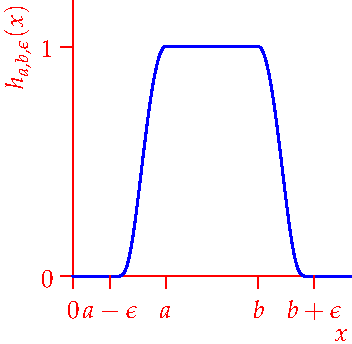
\includegraphics[scale=0.85]{diff-bump}
\end{minipage}
 	
 	\item\label{exs:binomialseries} (Hard) We prove the binomial series formula. Let $f(x)=(1+x)^\alpha$ and $g(x)=1+\sum\limits_{n=1}^\infty a_nx^n$ where $a_n=\frac{\alpha(\alpha-1)\cdots(\alpha-n+1)}{n!}$. Our goal is to prove that $f=g$ on the interval $(-1,1)$.
 	\begin{enumerate}
 	  \item Check that $f^{(n)}(0)=n!a_n$ so that $g$ really is the Maclaurin series of $f$.
 	  \item\begin{enumerate}
 	    	\item Prove that the radius of convergence of $g$ is 1.
 	  		\item Prove that $\lim\limits_{n\to\infty}na_nx^n=0$ whenever $\nm x<1$.
 	  		\item If $\nm x<1$ and $\xi$ lies between 0 and $x$, prove that $\nm{\frac{x-\xi}{1+\xi}}\le\nm x$.\\
 	  		(\emph{Hint: $\xi=tx$ for some $t\in(0,1)$\ldots})
 	  	\end{enumerate}
 	  \item Use Taylor's Theorem with Cauchy remainder to prove that
 	  \[\nm{R_n(x)}< (n+1)\nm{a_{n+1}}\nm x^{n+1}(1+\xi)^{\alpha-1}\]
 	  Hence conclude that $g=f$ whenever $\nm x<1$.
 	  \item Here is an alternative argument:
 	  \begin{enumerate}
 	    \item Show that $(n+1)a_{n+1}+na_n=\alpha a_n$.
 	    \item Differentiate term-by-term to prove directly that $g$ satisfies the differential equation $(1+x)g'(x)=\alpha g(x)$. Solve this to show that $g=f$ whenever $\nm x<1$.
 	  \end{enumerate}
 	\end{enumerate}
 	
\end{enumerate}
\end{exercises}



 
% 
% One use of this example is in the creation of \emph{bump functions,} which find great use throughout analysis. If $f$ is the above function and $a<b$, then we may define the function
% \[g_{a,b}:x\mapsto f(x-a)f(b-x)\]
% 
% \begin{minipage}[t]{0.6\linewidth}\vspace{0pt}
% This function is infinitely differentiable on $\R$ but is non-zero only on the interval $(a,b)$. With a little modification, one can even create an infinitely differentiable function on $\R$ which satisfies
% \[h_{a,b,\epsilon}(x)=\begin{cases}
% 0&\text{if $x\le a-\epsilon$ or $x\ge b+\epsilon$}\\
% 1&\text{if $a\le x\le b$}
% \end{cases}\]
% This `switches on' from 0 to 1 over an interval of width $\epsilon$ near $a$, then switches off with similar rapidity near $b$. As $\epsilon\to 0$ this approximates the indicator function for the interval $[a,b]$.
% \end{minipage}\begin{minipage}[t]{0.4\linewidth}\vspace{0pt}
% \flushright\includegraphics{diff-bump}
% \end{minipage}


% Indeed $g^{(n)}(\frac{a+b}2)=0$ for all $n\ge 1$, so one can even extend this: for any $a<b$ and $\epsilon>0$,
% \[h_{a,b,\epsilon}:x\mapsto \begin{cases}
% \frac 1{(g(a-\frac\epsilon 2))^2}g_{a-\epsilon,a}(x) & \text{if $x\in(a-\epsilon,a)$}\\
% 1&\text{if }a\le x\le b\\
% \frac 1{(g(b+\frac\epsilon 2))^2}g_{b,b+\epsilon}(x) & \text{if $x\in(b,b+\epsilon)$}\\
% 0 & \text{otherwise}
% \end{cases}\]
% 
% \begin{thm}[Taylor's theorem with integral remainder]
% Let $f$ be $n$ times differentiable on $(a,b)$ where $a<0<b$. Then for $x\in(a,b)$ we have
% \[R_n(x)=\int_0^x\frac{(x-t)^{n-1}}{(n-1)!}f^{(n)}(t)\D t.\tag*{$(\ast)$}\]
% \end{thm}
% 
% \begin{proof}
% We argue by induction. When $n=1$ we have $R_1(x)=f(x)-f(0)=\int_0^1f'(t)\D t$ (to be proved when we see the Fundamental Theorem of Calculus). Now assume that $(\ast)$ holds for some $n$. Then, by integration by parts (also to be justified later) we see that
% \begin{align*}
% R_n(x)&=\int_0^x\frac{(x-t)^{n-1}}{(n-1)!}f^{(n)}(t)\D t\\
% &=\left[-\frac{(x-t)^n}{n!}f^{(n)}(x)\right]_0^x+\int_0^x\frac{(x-t)^n}{n!}f^{(n+1)}(t)\D t\\
% &=\frac{x^n}{n!}f^{(n)}(x)+\int_0^x\frac{(x-t)^n}{n!}f^{(n+1)}(t)\D t.
% \end{align*}
% However this first term is precisely the difference $R_n(x)-R_{n+1}(x)$ from Definition \ref{defn:taylor}. Hence $(\ast)$ holds for $n+1$ and thus for all $n$ by induction.
% \end{proof}
% 
% Even though the result of the following example is easier to see directly from the previous corollary, we include it here for variety.
% 
% \begin{example}{}{}
% Let $f(x)=\sin x$. Then $\nm{f^{(n)}(x)}\le 1$ for all $x$. Hence
% \[\nm{R_n(x)}=\nm{\int_0^x\frac{(x-t)^{n-1}}{(n-1)!}f^{(n)}(t)\D t}\le\int_0^x\nm{\frac{(x-t)^{n-1}}{(n-1)!}}\D t=\frac{\nm x^n}{n!}\underset{n\to\infty}{\longrightarrow}0.\]
% Hence $\sin x$ is equal to its Taylor series for all $x\in\R$.




\graphicspath{{4int/asy/}}

\section{Integration}

The theory of infinite series addresses how to sum infinitely many \emph{finite} quantities. Integration, by contrast, is the business of summing infinitely many \emph{infinitesimal} quantities. Attempts to do both have been part of mathematics for well over 2000 years, and the philosophical objections are just as old.\footnote{%
	Two of Zeno's ancient paradoxes are relevant here: Achilles and the Tortoise concerns a convergent infinite series, while the Arrow Paradox toys with integration by questioning whether time can be viewed as a sum of instants. Perhaps the most famous contemporary criticism comes from Bishop George Berkeley, who gave his name to the city and first UC campus: in 1734's \href{https://en.wikipedia.org/wiki/The_Analyst}{\emph{The Analyst}}, Berkeley savaged the foundations of calculus, describing the infinitesimal increments required in Newton's theory of \emph{fluxions} (derivatives) as merely the ``ghosts of departed quantities.''%
} The development and increased application of calculus from the late 1600s onward spurred mathematicians to put the theory on a firmer footing, though from Newton and Leibniz it took another 150 years before Bernhard Riemann (1856) provided a thorough development of the integral.



\setcounter{subsection}{31}
\subsection{The Riemann Integral}\label{sec:riemann}

The basic idea behind Riemann integration is to approximate area using a sequence of rectangles whose \emph{width} tends to zero. The following discussion illustrates the essential idea, which should be familiar from elementary calculus.

\begin{example}[lower separated=false, sidebyside, sidebyside align=top seam, sidebyside gap=0pt, righthand width=0.37\linewidth]{}{riemannintro}
	Suppose $f(x)=x^2$ is defined on $[0,1]$.\medbreak
	For each $n\in\N$, let $\Delta x=\frac 1n$ and define $x_i=i\Delta x$.\smallbreak
	Above each \emph{subinterval} $[x_{i-1},x_i]$, raise a rectangle of height $f(x_i)=x_i^2$. The sum of the areas of these rectangles is the \emph{Riemann sum with right-endpoints}\footnotemark
	\begin{align*}
	  R_n&=\sum_{i=1}^n f(x_i)\Delta x 
	  =\sum_{i=1}^n\frac{i^2}{n^3}
	  =\frac{n(n+1)(2n+1)}{6n^3}\\ 
	  &=\frac 13+\frac{3n+1}{6n^2}
	\end{align*}
	
	The \emph{Riemann sum with left-endpoints} is defined similarly:
	\begin{align*}
	  L_n&=\sum_{i=1}^n f(x_{i-1})\Delta x 
	  =\sum_{i=1}^n\frac{(i-1)^2}{n^3} =\frac 13-\frac{3n-1}{6n^2}
	\end{align*}
	Since $f$ is an increasing function, the area $A$ under the curve plainly satisfies
	\[
		L_n\le A\le R_n
	\]
	By the squeeze theorem, we conclude that $A=\frac 13$.
	\tcblower
	\vspace{-5pt}
	\flushright\href{https://www.math.uci.edu/~ndonalds/math140b/riemann.html}{\includegraphics[scale=0.95]{area-up}\smallbreak
	\includegraphics[scale=0.95]{area-down}}
\end{example}

The example should feel convincing, though perhaps this is due to the simplicity of the function. To apply this approach to more general functions, we need to be significantly more rigorous.

\footnotetext{%
	Recall some basic identities:
	$\sum\limits_{i=1}^n i=\frac 12n(n+1)$, \ $\sum\limits_{i=1}^n i^2=\frac 16n(n+1)(2n+1)$, \ $\sum\limits_{i=1}^n i^3=\frac 14n^2(n+1)^2$%
}


\goodbreak


\begin{defn}{}{}
	A \emph{partition} $P=\{x_0,\ldots,x_n\}$ of an interval $[a,b]$ is a finite sequence for which
	\[
		a=x_0<x_1<\cdots< x_{n-1}< x_n=b
	\]
	Choosing a \emph{sample point} $x_i^*$ in each \emph{subinterval} $[x_{i-1},x_i]$ results in a \emph{tagged partition}.\smallbreak
	The \emph{mesh} of the partition is $\mesh(P):=\max\Delta x_i$, the width $\Delta x_i=x_i-x_{i-1}$ of the largest subinterval.\smallbreak
	If $f:[a,b]\to\R$, the \emph{Riemann sum} \smash{$\sum_{i=1}^n f(x_i^*)\,\Delta x_i$} evaluates the area of a family of $n$ rectangles, as pictured. The heights $f(x_i^*)$ and thus areas can be negative or zero.
	\begin{center}
	\includegraphics[scale=0.95]{riemann-sum}
	\end{center}
\end{defn}

In elementary calculus, one typically computes Riemann sums for \emph{equally-spaced} partitions with \emph{left,} \emph{right} or \emph{middle} sample points. The flexibility of tagged partitions makes applying Riemann's definition a challenge, so we instead consider two special families of rectangles. 


\begin{defn}{}{darbouxint}
	Given a partition $P$ of $[a,b]$ and a bounded function $f$ on $[a,b]$, define\par
	\begin{minipage}[t]{0.6\linewidth}\vspace{-15pt}
		\begin{align*}
			&M_i=\!\!\sup_{x\in [x_{i-1},x_i]}\! f(x)\qquad &&U(f,P)=\sum_{i=1}^n M_i\,\Delta x_i\\
			&m_i=\!\!\inf_{x\in [x_{i-1},x_i]}\! f(x) &&L(f,P)=\sum_{i=1}^n m_i\,\Delta x_i
		\end{align*}
		$U(f,P)$ and $L(f,P)$ are the \emph{upper} and \emph{lower Darboux sums} for $f$ with respect to $P$.
		The \emph{upper} and \emph{lower Darboux integrals} are
		% \begin{gather*}
		% U(f)=\upint_a^b f(x)\,\dx:=\inf\{U(f,P):P\text{ is a partition of $[a,b]$}\}\\
		% L(f)=\lowint_a^bf(x)\,\dx:=\sup\{L(f,P):P\text{ is a partition of $[a,b]$}\}
		% \end{gather*}
		\[
			U(f)=\inf U(f,P)\qquad L(f)=\sup L(f,P)
		\]
		where the supremum/infimum are taken over all partitions. Necessarily both integrals are \emph{finite.}\smallbreak
		We say that $f$ is \emph{(Riemann) integrable} on $[a,b]$ if $U(f)=L(f)$. We denote this value by
		\[
			\int_a^bf\quad\text{or}\quad\int_a^bf(x)\,\dx
		\]
		\end{minipage}
		\hfill
		\begin{minipage}[t]{0.39\linewidth}\vspace{-5pt}
			\centering
			\includegraphics[scale=0.95]{darboux-sum-upper}\par
			Upper Darboux sum $U(f,P)$\bigbreak
			\includegraphics[scale=0.95]{darboux-sum-lower}\par
			Lower Darboux sum $L(f,P)$
		\end{minipage}\medbreak
	If the interval is understood or irrelevant, one often simply says that $f$ is integrable and writes $\int f$.
	% We say that $f$ is integrable on a bounded interval $(a,b)$ if every extension of $f$ to $[a,b]$ is integrable.\smallbreak
\end{defn}


Intuitively, $L(f,P)$ is the sum of the areas of rectangles built on $P$ which just fit under the graph of $f$. It is also the infimum of all Riemann sums on $P$. If $f$ is discontinuous, then $L(f,P)$ need not itself be a Riemann sum, as there might not exist suitable sample points!

\goodbreak

\begin{examples}{}{}
	\exstart We revisit Example \ref{ex:riemannintro} in this language.
	\begin{enumerate}\setcounter{enumi}{1}
	  \item[]Given a partition $Q=\{x_0,\ldots,x_n\}$ of $[0,1]$ and sample points $x_i^*\in[x_{i-1},x_i]$, we compute the Riemann sum for $f(x)=x^2$
		\[
			\sum_{i=1}^nf(x_i^*)\,\Delta x_i=\sum_{i=1}^n(x_i^*)^2(x_i-x_{i-1})
		\]
		Since $f$ is increasing,  we have $x_{i-1}^2\le (x_i^*)^2\le x_i^2$ on each interval, whence
		\[
			L(f,Q) =\sum_{i=1}^n(x_{i-1})^2(x_i-x_{i-1})
			\le\sum_{i=1}^n(x_i^*)^2(x_i-x_{i-1})
			\le\sum_{i=1}^n(x_i)^2(x_i-x_{i-1})=U(f,Q)
		\]
		The Darboux sums are therefore the Riemann sums for left- and right-endpoints.\smallbreak
		If we take $Q_n$ to be the partition with subintervals of equal width $\Delta x=\frac 1n$, then
		\[
			U(f)=\inf_P U(f,P)\le U(f,Q_n)
			=\sum_{i=1}^n\left(\frac in\right)^2\!\Delta x =R_n
		\]
		is the right Riemann sum discussed originally. Similarly $L(f)\ge L_n$. Since $L_n$ and $R_n$ both converge to $\frac 13$ as $n\to \infty$, the squeeze theorem forces
		\[
			L_n\le L(f)\le U(f)\le R_n
			\implies L(f)=U(f)=\frac 13
		\]
		Otherwise said, $f$ is integrable on $[0,1]$ with $\int_0^1x^2\,\dx=\frac 13$.

		\begin{minipage}[t]{0.58\linewidth}\vspace{0pt}
			\item Suppose $f(x)=kx+c$ on $[a,b]$, and that $k>0$. Take the evenly spaced partition $P_n$ where $x_i=a+\frac{b-a}ni$. Since $f$ is increasing, the upper Darboux sum is again the Riemann sum with right-endpoints:
			\begin{align*}
				U(f,P_n)
				&=R_n=\sum_{i=1}^nf(x_i)\Delta x\\
				&=\frac{b-a}n\sum_{i=1}^n\frac{k(b-a)}ni+ak+c
			\end{align*}
		\end{minipage}
		\hfill
		\begin{minipage}[t]{0.4\linewidth}\vspace{0pt}
			\flushright\includegraphics[scale=0.95]{darboux-triangle}
		\end{minipage}\vspace{-5pt}
  
		\begin{align*}
			\phantom{U(f,P_n)}
			&=\frac{b-a}n\left[\frac{k(b-a)}n\cdot \frac 12n(n+1)+(ak+c)n\right]\\
			&\xrightarrow[n\to\infty]{} \frac 12k(b-a)^2+(b-a)(ak+c)
				=\frac k2(b^2-a^2)+c(b-a)
		\end{align*}
		Similarly, the lower Darboux sum is the Riemann sum with left-endpoints:
		\[
			L(f,P_n)=L_n
			=\frac{b-a}n\left[\frac{k(b-a)}n\cdot \frac 12n(n-1)+(ak+c)n\right] 
			\xrightarrow[n\to\infty]{} \frac k2(b^2-a^2)+c(b-a)
		\]
		As above, $L_n\le L(f)\le U(f)\le R_n$ and the squeeze theorem prove that $f$ is integrable on $[a,b]$ with $\int_a^bf=\frac k2(b^2-a^2)+c(b-a)$. 
	\end{enumerate}
\end{examples}

\goodbreak


\phantomsection\label{pg:riemanndefthm}
Now we have some examples, a few remarks are in order.
\begin{description}
  \item[\normalfont\emph{Riemann versus Darboux} ] Definition \ref{defn:darbouxint} is really that of the \emph{Darboux integral.} Here is Riemann's definition: $f:[a,b]\to\R$ being integrable with integral $\int_a^bf$ means
	\begin{gather*}
		\forall\epsilon>0,\ \exists\delta\text{ such that }(\forall P,x_i^*)\ \mesh(P)<\delta\implies \nm{\sum_{i=1}^nf(x_i^*)\Delta x_i-\int_a^bf}<\epsilon
	\end{gather*}
	This is significantly more difficult to work with, though it can be shown to be equivalent to the Darboux integral. We won't pursue Riemann's formulation further, except to observe that \emph{if} a function is integrable and $\mesh(P_n)\to 0$, then $\int_a^b f=\lim\limits_{n\to\infty}\sum_{i=1}^nf(x_i^*)\Delta x_i$: this allows us to approximate integrals using any sample points we choose, hence why \emph{right}-endpoints ($x_i^*=x_i$) are so common in Freshman calculus.
  \item[\normalfont\emph{Monotone Functions} ] Darboux sums are easy to compute for monotone functions. As in the examples, if $f$ is increasing, then each $M_i=f(x_i)$, from which $U(f,P)$ is the Riemann sum with \emph{right-endpoints.} Similarly, $L(f,P)$ is the Riemann sum with \emph{left-endpoints.} %The roles reverse if $f$ is decreasing.
  \item[\normalfont\emph{Area} ] If $f$ is positive and continuous,\footnote{%
  	We'll see in Theorem \ref{thm:monotoneint} that every continuous function is integrable.%
  } the Riemann integral $\int_a^bf$ serves as a \emph{definition} for the area under the curve $y=f(x)$. This should make intuitive sense:
  \begin{enumerate}
    \item In the second example where we have a straight line, we obtain the same value for the area by computing directly as the sum of a rectangle and a triangle!
    \item For any partition $P$, the area under the curve should satisfy the inequalities
  	\[
  		L(f,P)\le \text{Area}\le U(f,P)
  	\]
  	But these are precisely the same inequalities satisfied by the integral itself!
  	\[
  		L(f,P)\le L(f)=\int_a^bf=U(f)\le U(f,P)
  	\]
  \end{enumerate}
\end{description}


In the examples we exhibited a sequence of partitions $(P_n)$ where $U(f,P_n)$ and $L(f,P_n)$ converged to the same limit. The remaining results in this section develop some basic properties of partitions and make this limiting process rigorous.

\begin{defn}{}{}
	If $P\subseteq Q$ are both partitions of $[a,b]$, we call $Q$ a \emph{refinement} of $P$.
\end{defn}

To refine a partition, we simply throw some more points in! 

\begin{lemm}{}{partitionseqlemm}
	Suppose $f:[a,b]\to\R$ is bounded.
	\begin{enumerate}\itemsep2pt
	  \item If $Q$ is a refinement of $P$ (on $[a,b]$), then
	  \[
	  	L(f,P)\le L(f,Q)\le U(f,Q)\le U(f,P)
	  \]
	  \item For any partitions $P,Q$ of $[a,b]$, we have $L(f,P)\le U(f,Q)$.
	  \item $L(f)\le U(f)$
	\end{enumerate} 
\end{lemm}

\goodbreak

\begin{proof}
	\exstart We prove inductively. Suppose first that $Q=P\cup\{t\}$ contains exactly one additional point $t\in(x_{k-1},x_k)$. Write\par
	\begin{minipage}[t]{0.6\linewidth}\vspace{-15pt}
		\begin{enumerate}
		  \item[]\begin{gather*}
		  	m_1=\inf\bigl\{f(x):x\in[x_{k-1},t]\bigr\}\\
		  	m_2=\inf\big\{f(x):x\in[t,x_{k-1}]\bigr\}\\
		  	m=\inf\bigl\{f(x):x\in[x_{k-1},x_k]\bigr\}
		  	=\min\{m_1,m_2\}\\[-15pt]
		  \end{gather*}
		  The Darboux sums $L(f,P)$ and $L(f,Q)$ are identical except for the terms involving $t$. This results in \textcolor{Green}{extra area}:
	  \end{enumerate}
	\end{minipage}
	\hfill
	\begin{minipage}[t]{0.36\linewidth}\vspace{-17pt}
		\flushright\includegraphics[scale=0.95]{riemann-sum3}
	\end{minipage}
	\par\vspace{-17pt}
	
	\begin{enumerate}\setcounter{enumi}{1}
	  \item[]\begin{align*}
	  	\textcolor{Green}{L(f,Q)-L(f,P)} 
	  	&=m_1(t-x_{k-1}) +m_2(x_{k}-t) -m(x_k-x_{k-1})\\
	  	&=(m_1-m)(t-x_{k-1}) +(m_2-m)(x_k-t)
	  	\mathrel{\textcolor{Green}{\ge 0}}
	  \end{align*}
	  More generally, since a refinement $Q$ is obtained by adding \emph{finitely many} new points, induction tells us that $P\subseteq Q\Longrightarrow L(f,P)\le L(f,Q)$.\smallbreak
	  The argument for $U(f,Q)\le U(f,P)$ is similar, and the middle inequality is trivial.
	  
	  \item If $P$ and $Q$ are partitions, then $P\cup Q$ is a refinement of both $P$ and $Q$. By part 1,
	  \[
	  	L(f,P)\le L(f,P\cup Q)\le U(f,P\cup Q)\le U(f,Q)\tag{$\ast$}
	  \]
	  
		\item This is an exercise.\qedhere
	\end{enumerate}
\end{proof}


\begin{thm}{}{partitionseq}
	Suppose $f:[a,b]\to\R$ is bounded.
	\begin{enumerate}
	  \item\label{thm:partitionseq1} (Cauchy criterion)\lstsp $f$ is integrable $\Longleftrightarrow\forall\epsilon>0$, $\exists P$ such that $U(f,P)-L(f,P)<\epsilon$.
	  \item $f$ is integrable $\Longleftrightarrow\exists (P_n)_{n\in\N}$ such that $U(f,P_n)-L(f,P_n)\to 0$. In such a situation, both sequences $U(f,P_n)$ and $L(f,P_n)$ converge to $\int_a^bf$.
	\end{enumerate} 
\end{thm}

Part 1 is termed a `Cauchy' criterion since it doesn't mention the integral (limit). 


\begin{proof}
	We prove the Cauchy criterion, leaving part 2 as an exercise. 
	\begin{description}
		\item[$(\Rightarrow)$] Suppose $f$ is integrable and that $\epsilon>0$ is given. Since $\inf U(f,Q)=\int f=\sup L(f,R)$, there exist partitions $Q,R$ such that
		\[
			U(f,Q)<\int f+\frac\epsilon 2
			\quad\text{and}\quad 
			L(f,R)>\int f-\frac \epsilon 2
		\]
		Let $P=Q\cup R$ and apply ($\ast$): \ $L(f,R)\le L(f,P)\le U(f,P)\le U(f,Q)$. But then
		\[
			U(f,P)-L(f,P)\le U(f,Q)-L(f,R) 
			=U(f,Q)-\int f+\int f-L(f,R)<\epsilon
		\]
		\item[$(\Leftarrow)$] Assume the right hand side. For every partition, $L(f,P)\le L(f)\le U(f)\le U(f,P)$. Thus
		\[
			0\le U(f)-L(f)\le U(f,P)-L(f,P)<\epsilon
		\]
		Since this holds for all $\epsilon>0$, we see that $U(f)=L(f)$: that is, $f$ is integrable.\qedhere
	\end{description}
\end{proof}

\goodbreak


\begin{examples}{}{riemannint2}
	\exstart Consider $f(x)=\sqrt x$ on the interval $[0,b]$. We choose a sequence of partitions $(P_n)$ that evaluate nicely when fed to this function:
	\begin{gather*}
	  P_n=\{x_0,\ldots,x_n\}\quad\text{where}\quad x_i=\left(\frac in\right)^2b\\
	  \implies \Delta x_i=x_i-x_{i-1}=\frac b{n^2}\bigl(i^2-(i-1)^2\bigr)=\frac{(2i-1)b}{n^2}
	\end{gather*}
	Since $f$ is increasing on $[0,b]$, we see that
	\begin{align*}
	  U(f,P_n)
	  &=\sum_{i=1}^nf(x_i)\Delta x_i 
	  	=\sum_{i=1}^n\frac{i\sqrt b}n\cdot\frac{(2i-1)b}{n^2} 
	  	=\frac{b^{3/2}}{n^3}\sum_{i=1}^n2i^2-i \\
	  &=\frac{b^{3/2}}{n^3}\left[\frac 13n(n+1)(2n+1)-\frac 12n(n+1)\right] 
	  	\xrightarrow[n\to\infty]{}\frac 23b^{3/2}
	\end{align*}
	Similarly
	\begin{align*}
	  L(f,P_n)
	  &=\sum_{i=1}^nf(x_{i-1})\Delta x_i 
	  	=\sum_{i=1}^n\frac{(i-1)\sqrt b}n\cdot\frac{(2i-1)b}{n^2} 
	  	=\frac{b^{3/2}}{n^3}\sum_{i=1}^n2i^2-3i+1 \\
	  &=\frac{b^{3/2}}{n^3}\left[\frac 13n(n+1)(2n+1)-\frac 32n(n+1) +n\right] 
	  	\xrightarrow[n\to\infty]{}\frac 23b^{3/2}
	\end{align*}
	Since the limits are equal, we conclude that $f$ is integrable and $\int_0^b\sqrt x\,\dx=\frac 23b^{3/2}$.
	
	\begin{enumerate}\setcounter{enumi}{1}
	  \item[]\begin{center}
		  \begin{tabular}{c@{\qquad}c}
		  	\includegraphics[scale=0.95]{darboux-ex1}
		  	&
		  	\includegraphics[scale=0.95]{darboux-ex2}
	  	\end{tabular}
	  \end{center}
	  
		\item\label{ex:riemannint2nonint} Here is the classic example of a \emph{non-integrable function}. Let $f:[a,b]\to\R$ to be the indicator function of the irrational numbers,
		\[
			f(x)=
			\begin{cases}
				1&\text{if }x\not\in\Q\\
				0&\text{if }x\in\Q
			\end{cases}
		\]
		Suppose $P=\{x_0,\ldots,x_n\}$ is \emph{any} partition of $[a,b]$. Since any interval of positive length contains both rational and irrational numbers, we see that
		\begin{gather*}
			\sup\bigl\{f(x):x\in[x_{i-1},x_i]\bigr\} =1 \implies U(f,P)=\sum_{i=1}^n(x_i-x_{i-1})=b-a\implies U(f)=b-a\\
			\inf\bigl\{f(x):x\in[x_{i-1},x_i]\bigr\}=0 \implies L(f,P)=0\implies L(f)=0
		\end{gather*}
		Since the upper and lower Darboux integrals differ, $f$ is not (Riemann) integrable.
	\end{enumerate}
\end{examples}


% \begin{asidep}
% The definition we have given is strictly that of the \emph{Darboux integral}. Riemann's definition is as follows:
% 
% \begin{defn}
% Let $f$ be bounded on $[a,b]$ and let $P$ be a partition. A \emph{Riemann sum} of $f$ associated to $P$ is a sum
% \[\sum_{k=1}^nf(x_k)(t_k-t_{k-1}),\text{ where }x_k\in[t_{k-1},t_k].\]
% $f$ is \emph{Riemann integrable} on $[a,b]$ with integral $r$ if for all $\epsilon>0$ there exists $\delta>0$ such that for all Riemann sums $S$ with partitions finer than $\delta$ (i.e. $t_k-t_{k-1}<\delta$ for all $k$) we have
% \[\nm{S-r}<\epsilon.\]
% \end{defn}
% 
% It is common to use the term Riemann integral for either Riemann's or Darboux's definition since they coincide (by contrast, alternative definitions of the integral allow more functions to be considered integrable). Indeed we have the following theorem:
% 
% \begin{thm}
% $f$ is Riemann integrable on $[a,b]$ iff it is Darboux integrable on $[a,b]$, in which case the values of the integrals coincide.
% \end{thm}
% 
% In order to prove the theorem, and several others in the next section, it is convenient to have the following definition and $\epsilon$--$\delta$ criterion for integrability, which we state without its uninstructive proof.
% 
% \begin{defn}
% Given a partition $P=\{t_0<\cdots<t_n\}$ of $[a,b]$, the \emph{mesh} of $P$ is the maximum of the distances between successive $t_k$. I.e. $\mesh(P)=\max(t_k-t_{k-1})$.
% \end{defn}
% 
% \begin{prop}\label{prop:intepsilon}
% A bounded function $f$ on $[a,b]$ is integrable iff either of the following conditions hold:
% \begin{enumerate}
%   \item For each $\epsilon>0$ there exists a partition $P$ of $[a,b]$ such that
% \[U(f,P)-L(f,P)<\epsilon.\]
% \item For all $\epsilon>0$ there exists $\delta>0$ such that
% \[\mesh(P)<\delta\Longrightarrow U(f,P)-L(f,P)<\epsilon.\]
% \end{enumerate}
% \end{prop}
% 
% The proposition is intuitive in the sense that we visualize the upper and lower Darboux sums as converging to the integral. This is, of course, not technically correct, since there is no sequence of Darboux sums.
% 
% \begin{proof}[Proof of Theorem]
% Suppose $f$ is Darboux integrable and let $\epsilon>0$ be chosen. Let $\delta>0$ be chosen satisfying Proposition \ref{prop:intepsilon}. Let $P$ be any partition of $[a,b]$ with $\mesh(P)<\delta$ and let $S$ be a Riemann sum associated to $P$. Clearly we have
% \[L(f,P)\le S\le U(f,P).\]
% By Proposition \ref{prop:intepsilon} we have
% \[U(f,P)<L(f,P)+\epsilon\le L(f)+\epsilon.\]
% Similarly
% \[L(f,P)>U(f,P)-\epsilon\ge U(f)-\epsilon.\]
% Since $U(f)=L(f)=\int_a^bf$ we see that
% \[\int_a^bf-\epsilon<S<\int_a^b+\epsilon.\]
% Hence $f$ is Riemann integrable, with integral $r=\int_a^bf$.\\
% Now suppose $f$ is Riemann integrable with integral $r$. Let $\epsilon>0$ be given, $\delta>0$ satisfying the definition and $P$ a partition finer than $\delta$. Then any Riemann sum associated to $P$ satisfies
% \[\nm{S-r}<\epsilon.\]
% Since $\epsilon>0$ we may select $x_k\in[t_{k-1},t_k]$ such that
% \[f(x_k)>\sup\{f(x):x\in[t_{k-1},t_k]\}-\epsilon.\]
% The Riemann sum $S$ for these $x_i$ clearly satisfies
% \[S\ge U(f,P)-\epsilon(b-a).\]
% But then, for all $\epsilon>0$ we have
% \[U(f)\le U(f,P)\le S+\epsilon(b-a)\le r+\epsilon+\epsilon(b-a)=r+\epsilon(1+b-a),\]
% so that $U(f)\le r$. Similarly we see that $L(f)\ge r$. Then $U(f)\ge L(f)$ implies equality and so $f$ is Darboux integrable with integral $\int_a^bf=r$.
% \end{proof}
% \end{asidep}\newpage

As any freshman calculus student can attest, if you can find an anti-derivative, then the fundamental theorem of calculus (Section \ref{sec:ftc}) makes evaluating integrals far easier. For instance, you are probably desperate to write
\[
	\diff x\frac 23x^{3/2}=x^{1/2}
	\implies \int_0^b\sqrt x\,\dx
	=\frac 23x^{3/2}\Big|_0^b
	=\frac 23b^{3/2}
\]
rather than computing Riemann/Darboux sums as in the previous example! However, in most practical situations, no easy-to-compute anti-derivative exists; the best we can do is to approximate using Riemann sums for progressively finer partitions. Thankfully computers excel at such tedious work!


\begin{exercises}
	\emph{Key concepts:\quad Darboux sums/integrals,\qquad Partitions, sample points \& refinements,}
	\begin{quote}
		\emph{Cauchy \& sequential criteria for integrability}
	\end{quote}
	
	\begin{enumerate}
		\item\label{exs:easydarbint} Use partitions to find the upper and lower Darboux integrals on the interval $[0,b]$. Hence prove that the function is integrable and compute its integral.
		\begin{enumerate}
		  \item $f(x)=x^3$\qquad\qquad\qquad (b) \ $g(x)=\sqrt[3]{x}$%\par
		  %(\emph{Hint: mimic Example \hyperref[ex:riemannint2]{\ref*{ex:riemannint2}.1})}
		\end{enumerate}
		
		
		\item Repeat question \ref*{exs:easydarbint} for the following two functions. You cannot simply compute Riemann sums for left and right endpoints and take limits: why not?
		\begin{enumerate}  
		  \item $h(x)=x(2-x)$ on $[0,2]$\smallbreak
		  (\emph{Hint: choose a partition with $2n$ points such that $x_n=1$ and observe that $h(2-x)=h(x)$})
		  
		  \item On the interval $[0,3]$, let $k(x)=\begin{cases}
		  2x&\text{if }x\le 1\\
		 	5-x&\text{if }x>1
		  \end{cases}$\smallbreak
		  (\emph{Hint: this time try a partition with $3n$ points})
		\end{enumerate}
	
	
	  \item Let $f(x)=x$ for rational $x$ and $f(x)=0$ for irrational $x$. Calculate the upper and lower Darboux integrals for $f$ on the interval $[0,b]$. Is $f$ integrable on $[0,b]$?
	
	    
		\item Prove part 3 of Lemma \ref{lemm:partitionseqlemm}: $L(f)\le U(f)$.
	
	
		\item Prove part 2 of Theorem \ref{thm:partitionseq}.
	 	\begin{quote}
	 		$f$ is integrable $\iff\exists (P_n)_{n\in\N}$ such that $\lim\limits_{n\to\infty}\bigl(U(f,P_n)-L(f,P_n)\bigr) =0$
	 	\end{quote}
	 	Moreover, prove that both $U(f,P_n)$ and $L(f,P_n)$ converge to $\int f$.
		
		\item\begin{enumerate}
		  \item Reread Definition \ref{defn:darbouxint}. What happens if we allow $f:[a,b]\to\R$ to be \emph{unbounded}?
		  \item (Hard)\lstsp Read ``\emph{Riemann versus Darboux}'' on page \pageref{pg:riemanndefthm}. Explain why being \emph{Riemann} integrable also forces $f$ to be bounded.
		  \item (Hard)\lstsp Explain the observation that $L(f,P)$ is the infimum of the set of all Riemann sums on $P$.
		\end{enumerate}
	
		\item (If you like coding)\quad Write a short program to estimate $\int_a^bf(x)\,\dx$ using Riemann sums. This can be very simple (equal partitions with right endpoints), or more complex (random partition and sample points given a mesh). Apply your program to estimate $\int_0^{5}\sin(x^2e^{-\sqrt x})\,\dx$.
	\end{enumerate}
\end{exercises}



\clearpage



\subsection{Properties of the Riemann Integral}\label{sec:riemannproperties}

The rough take-away of this long section is that everything you think is integrable probably is! Examples will be few, since we have not established many explicit values for integrals.


\begin{thm}{Linearity}{intlinear}
	If $f,g$ are integrable and $k,l$ are constant, then $kf+lg$ is integrable and
	\[
		\int  kf+lg=k\int f+l\int g
	\]
\end{thm}

\begin{example}{}{}
Thanks to examples in the previous section, we can now calculate, e.g.,
\[
	\int_0^25x^3-3\sqrt x\,\dx
	=5\cdot\frac 14\cdot 2^4 -3\cdot \frac 23\cdot 2^{3/2} 
	=20-4\sqrt 2
\]
\end{example}

\begin{proof}
	Suppose $\epsilon>0$ is given. By the Cauchy criterion (Theorem \ref{thm:partitionseq}, part \ref*{thm:partitionseq1}), there exist partitions $R,S$ such that
	\[
		U(f,R)-L(f,R)<\smash{\frac\epsilon 2}
		\quad\text{and}\quad 
		U(g,S)-L(g,S)<\smash{\frac\epsilon 2}
	\]
	If $P=R\cup S$, then both inequalities are satisfied by $P$ (Lemma \ref{lemm:partitionseqlemm}). On each subinterval,
	\[
		\inf f(x)+\inf g(x)\le \inf\bigl(f(x)+g(x)\bigr)
		\quad\text{and}\quad 
		\sup\bigl(f(x)+g(x)\bigr)\le\sup f(x)+\sup g(x)
	\]
	since the individual suprema/infima could be `evaluated' at different places. Thus
	\[
		L(f,P)+L(g,P)\le L(f+g,P)\le U(f+g,P)\le U(f,P)+U(g,P)
	\]
	whence $U(f+g,P)-L(f+g,P)<\epsilon$ and $f+g$ is integrable. Moreover,
	\[
		\int(f+g)-\int f-\int g \le \Bigl(U(f,P)-\int f\Bigr)+\Bigl(U(g,P)-\int g\Bigr)<\epsilon
	\]
	Using lower Darboux integrals similarly obtains the other half of the inequality
	\[
		-\epsilon<\int(f+g)-\int f-\int g<\epsilon
	\]
	Since this holds for all $\epsilon>0$, we conclude that $\int(f+g)=\int f+\int g$.\smallbreak
	That $kf$ is integrable with $\int kf=k\int f$ is an exercise. Put these together for the result.
\end{proof}


\begin{cor}{Changing endvalues}{intopen}
	Suppose $f$ is integrable on $[a,b]$ and $g:[a,b]\to\R$ satisfies $f(x)=g(x)$ on $(a,b)$. Then $g$ is also integrable on $[a,b]$ and $\int_a^b g=\int_a^b f$.
\end{cor}


\begin{defn}{Integration on an open interval}{intopen}
	A \emph{bounded} function $g:(a,b)\to\R$ is \emph{integrable} if it has an integrable extension $f:[a,b]\to\R$ where $f(x)=g(x)$ on $(a,b)$.
	In such a case, we define $\int_a^bg:=\int_a^bf$.
\end{defn}

The Corollary (its proof is an exercise) shows that the choice of extension is irrelevant.


\goodbreak


\begin{thm}{Basic integral comparisons}{intineq}
	Suppose $f$ and $g$ are integrable on $[a,b]$. Then:
	\begin{enumerate}\itemsep1pt\parsep=1pt
	  \item $f(x)\le g(x) \Longrightarrow\int f\le\int g$
	  \item $m\le f(x)\le M\Longrightarrow m(b-a)\le\int_a^bf\le M(b-a)$
	  \item $fg$ is integrable.
	  \item $\nm f$ is integrable and $\nm{\int f}\le\int \nm f$
	  \item $\max(f,g)$ and $\min(f,g)$ are both integrable.
	\end{enumerate}
\end{thm}

Part 3 is \emph{not} integration by parts since it doesn't tell us how $\int fg$ relates to $\int f$ and $\int g$!

\begin{proof}
	\begin{enumerate}\itemsep=1pt\parsep=1pt
	  \item Since $g-f$ is positive and integrable, $L(g-f,P)\ge 0$ for all partitions $P$. But then
	  \[
	  	\smash{0\le \inf L(g-f,P)=L(g-f)=\int g-f=\int g-\int f}
	  \]
	  \item Apply part 1 twice.
	  \item This is an exercise.
	  \item The integrability is an exercise. For the comparison, apply part 1 to $-\nm f\le f\le\nm f$.
	  \item Use $\max(f,g)=\frac 12(f+g)+\frac 12\nm{f-g}$, etc., together with the previous parts.\qedhere
	\end{enumerate}
\end{proof}


\begin{thm}[lower separated=false, sidebyside, sidebyside align=top seam, sidebyside gap=0pt, righthand width=0.35\linewidth]{Domain splitting}{domainsplit}
	Suppose $f:[a,b]\to\R$ and let $c\in(a,b)$. If $f$ is integrable on both $[a,c]$ and $[c,b]$, then it is integrable on $[a,b]$ and
	\[
		\int_a^bf=\int_a^cf+\int_c^bf
	\]
	\tcblower
	\flushright\includegraphics[scale=0.95]{domain-split}
\end{thm}

In light of this result, it is conventional to allow integral limits to be reversed: if $a<b$, then
\[
	\int_b^af:=-\int_a^bf
	\quad\text{ is consistent with }\quad 
	\int_a^af=0
\]


\begin{proof}
	Let $\epsilon>0$ be given, then $\exists R,S$ partitions of $[a,c],[c,b]$ such that\par
	\begin{minipage}[t]{0.65\linewidth}\vspace{-10pt}
		\[
			U(f,R)-L(f,R)<\frac\epsilon 2,\qquad U(f,S)-L(f,S)<\frac\epsilon 2
		\]
		Choose $P=R\cup S$ to partition $[a,b]$, then
		\[
			U(f,P)-L(f,P)=U(f,R)+U(f,S)-L(f,R)-L(f,S)<\epsilon
		\]
		Moreover
	\end{minipage}
	\hfill
	\begin{minipage}[t]{0.34\linewidth}\vspace{0pt}
		\flushright\includegraphics[scale=0.95]{domain-split2}
	\end{minipage}\par
	\[
		\int_a^bf-\int_a^cf-\int_c^bf
		\le U(f,P)-L(f,R)-L(f,S)
		=U(f,P)-L(f,P)<\epsilon
	\]
	Showing that this expression is greater than $-\epsilon$ is similar.
\end{proof}


\goodbreak


\begin{example}{}{}
	If $f(x)=\sqrt x$ on $[0,1]$ and $f(x)=1$ on $[1,2]$, then
	\[
		\int_0^2f =\int_0^1\sqrt x\,\dx+\int_1^2 1\,\dx
		=\frac 23+1 =\frac 53
	\]
\end{example}


\boldinline{Monotonic \& Continuous Functions}

We establish the integrability of two large classes of functions.

\begin{defn}{}{}
	A function $f:[a,b]\to\R$ is:
	\begin{description}\itemsep1pt
		\item[\normalfont\emph{Monotonic}] if it is either \emph{increasing} ($x<y\Longrightarrow f(x)\le f(y)$) or \emph{decreasing}.
		\item[\normalfont\emph{Piecewise monotonic}] if there is a partition $P=\{x_0,\ldots,x_n\}$ (finite!) of $[a,b]$ such that $f$ is monotonic on each open subinterval $(x_{k-1},x_k)$.
		\item[\normalfont\emph{Piecewise continuous}] if there is a partition such that $f$ is \emph{uniformly continuous} on each $(x_{k-1},x_k)$.
	\end{description}
\end{defn}


\begin{thm}{}{monotoneint}
	If $f$ is \emph{monotonic} or \emph{continuous} on $[a,b]$, then it is integrable.
\end{thm}


\begin{examples}{}{}
	\exstart Since sine is continuous, we can approximate via a sequence of Riemann sums
	\[
		\int_0^\pi\sin x\,\dx 
		=\frac\pi{n}\lim_{n\to\infty}\sum_{i=1}^n\sin\frac{\pi i}n
	\]
	\emph{Evaluating} this limit is another matter entirely, one best handled in the next section...\vspace{-3pt}
	\begin{enumerate}\setcounter{enumi}{1}
	  \item Similarly, $e^{\sqrt x}$ is integrable and therefore may be approximated via Riemann sums:
	  \[
	  	\int_0^1 e^{\sqrt x}\,\dx 
	  	=\frac 1{n}\lim\limits_{n\to\infty}\sum_{i=1}^n \exp\sqrt{\frac in} 
	  	=\lim\limits_{n\to\infty}\sum_{j=1}^n \frac{2j-1}n\exp\frac jn
	  \]
	  Both sums use right endpoints: the first has equal subintervals, while the second is analogous to Example \ref{ex:riemannint2}.1. These limits would typically be estimated using a computer.
	\end{enumerate}
\end{examples}

\begin{proof}
	Since $[a,b]$ is closed and bounded, a continuous function $f$ is \emph{uniformly} so. Let $\epsilon>0$ be given:
	\[
		\exists\delta>0\text{ such that }
		\forall x,y\in[a,b],\ 
		\nm{x-y}<\delta \implies \nm{f(x)-f(y)}<\frac\epsilon{b-a}
	\]
	Let $P$ be a partition with $\mesh P<\delta$. Since $f$ attains its bounds on each $[x_{i-1},x_i]$,
	\[
		\exists x_i^*,y_i^*\in [x_{i-1},x_i]
		\quad\text{such that}\quad 
		M_i-m_i=f(x_i^*)-f(y_i^*)<\frac\epsilon{b-a}
	\]
	from which
	\[
		U(f,P)-L(f,P)
		<\smash[t]{\sum_{i=1}^n}\frac\epsilon{b-a}(x_i-x_{i-1})
		=\epsilon
	\]
	The monotonicity argument is an exercise.
\end{proof}

Combining the proof with Definition \ref{defn:intopen}: every \emph{uniformly continuous} $f:(a,b)\to\R$ is integrable.

\goodbreak


\begin{cor}{}{piecewiseint}
	Piecewise continuous and \textbf{bounded} piecewise monotonic functions are integrable.
\end{cor}


\begin{proof}
	If $f$ is piecewise continuous, then the restriction of $f$ to $(x_{k-1},x_k)$ has a continuous extension $g_k:[x_{k-1},x_k]\to\R$; this is integrable by Theorem \ref{thm:monotoneint}. By Corollary \ref{cor:intopen}, $f$ is integrable on $[x_{k-1},x_k]$ with $\int_{x_{k-1}}^{x_k}f=\int_{x_{k-1}}^{x_k}g_k$. Theorem \ref{thm:domainsplit} ($n-1$ times!) finishes things off:
	\[
		\int_a^bf=\sum_{k=1}^n\int_{x_{k-1}}^{x_k}f
	\]
	The argument for piecewise monotonicity is similar.
\end{proof}


\begin{example}[lower separated=false, sidebyside, sidebyside align=top seam, sidebyside gap=0pt, righthand width=0.35\linewidth]{}{fracpart}
	The `fractional part' function $f(x)=x-\lfloor x\rfloor$ is both piecewise continuous and piecewise monotone on any bounded interval. It is therefore integrable on any such interval.
	\tcblower
	\flushright\includegraphics{fracpart}
\end{example}


For a final corollary, here is one more incarnation of the intermediate value theorem.

\begin{cor}{IVT for integrals}{}
	If $f$ is continuous on $[a,b]$, then $\exists \xi\in (a,b)$ for which
	\[
		f(\xi)=\frac 1{b-a}\int_a^bf
	\]
\end{cor}

\begin{proof}
	Since $f$ is continuous, it is integrable on $[a,b]$. By the extreme value theorem it is also bounded and attains its bounds: $\exists p,q\in[a,b]$ such that\par
	\begin{minipage}[t]{0.55\linewidth}\vspace{-5pt}
		\[
			f(p):=\inf\limits_{x\in[a,b]}f(x),\qquad f(q)=\sup\limits_{x\in[a,b]}f(x)
		\]
		Applying Theorem \ref{thm:intineq}, part 2, with $m=f(p)$ and $M=f(q)$, we see that
		\[
			(b-a)f(p)\le\int_a^bf\le (b-a)f(q)
		\]
	\end{minipage}
	\hfill
	\begin{minipage}[t]{0.44\linewidth}\vspace{-5pt}
		\flushright\includegraphics[scale=0.95]{average}
	\end{minipage}\bigbreak

	Divide by $b-a$ and apply the usual intermediate value theorem for $f$ to see that the required $\xi$ exists between $p$ and $q$.
\end{proof}

In the picture, when $f$ is positive and continuous, the grey area equals that under the curve; imagine levelling off the blue hill with a bulldozer\ldots{} The notation $\textcolor{orange}{f_{\text{av}}}=\frac 1{b-a}\int_a^bf$ indicates the \textcolor{orange}{average value} of $f$ on $[a,b]$: to see why this interpretation is sensible, take a sequence of Riemann sums on equally-spaced partitions $P_n$ to see that
\[
	\frac 1{b-a}\int_a^b f 
	=\lim_{n\to\infty}\sum_{i=1}^nf(x_i^*)\Delta x
	=\lim_{n\to\infty}\frac{f(x_1^*)+\cdots+f(x_n^*)}n
\]
is the limit of a sequence of \emph{averages} of equally-spaced samples $f(x_i^*)$.


\goodbreak


\boldsubsubsection{What can/cannot be integrated?}

We now know a great many examples of integrable functions:
\begin{itemize}\itemsep0pt
  \item Piecewise continuous \& monotonic functions are integrable.
  \item Linear combinations, products, absolute values, maximums and minimums of (already) integrable functions.
\end{itemize}

By contrast, we've only seen one non-integrable function (Example \ref*{ex:riemannint2}.\ref{ex:riemannint2nonint}). After so many positive integrability conditions, it is reasonable to ask precisely which functions are Riemann integrable. Here is the answer, though it is quite tricky to understand.

\begin{thm}{Lebesgue}{lebesgue}
	Suppose $f:[a,b]\to\R$ is bounded. Then
	\begin{quote}
		$f$ is Riemann integrable $\iff$ it is continuous except on a set of \emph{measure zero}
	\end{quote}
\end{thm}

Naïvely, the \emph{measure} of a set is the sum of the lengths of its maximal subintervals, though unfortunately this doesn't make for a very useful definition.\footnote{%
	Formally, the \emph{length} of an open interval $(a,b)$ is $b-a$ and a set $A\subseteq \R$ has \emph{measure zero} if
	\[
		\forall\epsilon>0,\ \exists \text{ open intervals $I_n$ such that }
		A\subseteq\bigcup_{n=1}^\infty I_n
		\text{ and }
		\sum_{i=1}^\infty\operatorname{length}(I_n)<\epsilon
	\]
	More generally, the \emph{Lebesgue measure} of a set (subject to a technical condition) is the infimum of the sum of the lengths of any countable collection of open covering intervals. \emph{Measure theory} is properly a matter for graduate study.	Surprisingly, there exist \href{https://en.wikipedia.org/wiki/Smith-Volterra-Cantor_set}{sets} with positive measure that contain no subintervals, and even sets which are non-measurable!%
}
Any countable subset has measure zero, so Lebesgue's result is almost as if we can extend Corollary \ref{cor:piecewiseint} to allow for infinite sums. For instance, Exercise \ref*{sec:cont}.\ref{exs:discontq} describes a function which is continuous only on the irrationals: it is thus Riemann integrable (indeed $\int_a^bf=0$ for any $a<b$). There are also uncountable sets with measure zero such as Cantor's middle-third set $\mathcal C$: the function
\[
	f(x)=
	\begin{cases}
		1&\text{if }x\in\mathcal C\\
		0&\text{otherwise}
	\end{cases}
\]
is continuous except on $\mathcal C$ and therefore Riemann integrable; again $\int_0^1 f(x)\,\dx=0$.


\vfil

\begin{exercises}
	\emph{Key concepts:\quad Linear combinations, products, etc., of integrable functions are integrable,}\vspace{-5pt}
 	\begin{quote}
 		\emph{Continuous and monotone functions are integrable,\qquad Integrability on open intervals}
 	\end{quote}


	\begin{enumerate}
	  \item Explain why $\int_{0}^{2\pi}x^2\sin^8(e^x)\,\dx \le\frac 83\pi^3$
	  
	  
		\item If $f$ is integrable on $[a,b]$ prove that it is integrable on any interval $[c,d]\subseteq[a,b]$.
		
		
		\item We complete the proof of Theorem \ref{thm:intlinear} (linearity of integration).
		\begin{enumerate}
	  	\item Suppose $k>0$, let $A\subseteq\R$ and define $kA:=\{kx:x\in A\}$. Prove that $\sup kA=k\sup A$ and $\inf kA=k\inf A$.
	  	\item If $k>0$ prove that $kf$ is integrable on any interval and that $\int kf=k\int f$.
	  	\item How should you modify your argument if $k<0$?
		\end{enumerate}
		
	  
	  \item Give an example of an integrable but \emph{discontinuous} function on a closed bounded interval $[a,b]$ for which the conclusion of the Intermediate Value Theorem for Integrals is \emph{false.}
	  
	  
		\item Use Darboux sums to compute the value of the integral $\int_{1/2}^{{15/2}} x-\lfloor x\rfloor \,\dx$ (Example \ref{ex:fracpart}).
		
		
		\item\label{exs:extensionlemma} We prove and extend Corollary \ref{cor:intopen}. Suppose $f$ is integrable on $[a,b]$. 
		\begin{enumerate}
		  \item If $g:[a,b]\to\R$ satisfies $f(x)=g(x)$ for all $x\in (a,b)$, prove that $g$ is integrable and $\int_a^bg=\int_a^bf$.\smallbreak
			(\emph{Hint: consider $h=f-g$ and show that $\int h=0$})
			\item Now suppose $g:[a,b]\to\R$ satisfies $f(x)=g(x)$ for all $x\in [a,b]$ except at finitely many points. Prove that $g$ is integrable and $\int_a^bg=\int_a^bf$.
		\end{enumerate}
	  
	  
	  \item Show that an increasing function on $[a,b]$ is integrable and thus complete Theorem \ref{thm:monotoneint}.\par
	  (\emph{Hint: Choose a partition with $\mesh P<\frac\epsilon{f(b)-f(a)}$})
	 
	  
	  \item Suppose $f$ and $g$ are integrable on $[a,b]$.
		\begin{enumerate}
	    \item Define $h(x)=\bigl(f(x)\bigr)^2$. We know:
	  	\begin{itemize}
	    	\item $f$ is bounded: $\exists K$ such that $\nm{f(x)}\le K$ on $[a,b]$.
	    	\item Given $\epsilon>0$, $\exists P$ such that $U(f,P)-L(f,P)<\frac\epsilon{2K}$.
	  		For each subinterval $[x_{i-1},x_i]$, let
	  		\[
	  			M_i=\sup f(x),\qquad m_i=\inf f(x),\qquad 
	  			\cl M_i=\sup h(x),\qquad \cl m_i=\inf h(x)
	  		\]
	  	\end{itemize}
	  	Prove that $\cl M_i-\cl m_i\le 2(M_i-m_i)K$. Hence conclude that $h$ is integrable.
	  	
	  	\item Prove that $fg$ is integrable.\par
	  	(\emph{Hint: $fg=\frac 14(f+g)^2-\frac 14(f-g)^2$})
	  	
	  	\item Prove that $U(\nm f,P)-L(\nm f,P)\le U(f,P)-L(f,P)$ for any partition $P$. Hence conclude that $\nm f$ is integrable.
	  \end{enumerate}

	  (\emph{One can extend these arguments to show that if $j$ is continuous, then $j\circ f$ is integrable. Parts (a) and (c) correspond, respectively, to $j(x)=x^2$ and $j(x)=\nm x$.})
	  
	  
	  \item (Hard)\quad Let $f(x)=
	  \begin{cases}
	  	x&\text{if }x\neq 0\text{ and }\sin\frac 1x>0\\
	  	-x&\text{if }x\neq 0\text{ and }\sin\frac 1x<0\\
	  	0&\text{if }x=0 
	  \end{cases}$
	  \begin{enumerate}
	  	\item Show that $f$ is not piecewise continuous on $[0,1]$.
	  	
	    \item Show that $f$ is not piecewise monotonic on $[0,1]$.
	    
	    \item Show that $f$ is integrable on $[0,1]$.\par
	    (\emph{Hint: given $\epsilon$, hunt for a suitable partition to make $U(f,P)-L(f,P)<\epsilon$ by considering $[0,x_1]$ differently to the other subintervals})
	    
	    \item Make a similar argument which proves that $g=\sin\frac 1x$ is integrable on $(0,1]$.\par
	    (\emph{Hint: Show that $g$ has an integrable extension on $[0,1]$})
	  \end{enumerate}
	
	\end{enumerate}
\end{exercises}


\clearpage


\subsection{The Fundamental Theorem of Calculus}\label{sec:ftc}

The key result linking integration and differentiation is usually presented in two parts. While there are significant subtleties, the rough statements are as follows (we follow the traditional numbering):

\begin{description}
	\item[\normalfont\emph{Part I} ] Differentiation reverses integration: $\diff x\int_a^xf(t)\,\dt=f(x)$
	\item[\normalfont\emph{Part II} ] Integration reverses differentiation: $\int_a^bF'(x)\,\dx =F(b)-F(a)$
\end{description}

\begin{minipage}[t]{0.7\linewidth}\vspace{-10pt}
	These facts seemed intuitively obvious to early practitioners of calculus. Given a continuous positive function $f$:
	\begin{itemize}
	  \item Let $F(x)$ denote the area under $y=f(x)$ between $0$ and $x$. 
	  \item A small increase $\Delta x$ results in the area increasing by $\Delta F$.
	  \item $\Delta F\approx f(x)\Delta x$ is approximately the area of a rectangle, whence $\frac{\Delta F}{\Delta x}\approx f(x)$. This is part I.
	  \item $F(b)-F(a)\approx\sum \Delta F_i\approx \sum f(x_i)\Delta x_i$. Since $F'=f$, this is part II.
	\end{itemize}
\end{minipage}
\hfill
\begin{minipage}[t]{0.29\linewidth}\vspace{-10pt}
	\flushright\includegraphics[scale=0.95]{ftcold}
\end{minipage}\medbreak

When Leibniz introduced the symbols $\int$ and $\D$ in the late 1600s, it was partly to reflect the fundamental theorem.\footnote{%
	\def\dF{\D F}$\int$ is a stylized S for \emph{sum,} while $\D$ stands for \emph{difference.} Given a sequence $F=(F_0,F_1,F_2,\ldots,F_n)$, construct a new sequence of \emph{differences}
	\[
		\dF=(F_1-F_0,F_2-F_1,\ldots,F_n-F_{n-1})
	\]
	which can then be summed:
	\[
		\int\dF=(F_1-F_0)+(F_2-F_1)+\cdots (F_n-F_{n-1})=F_n-F_0 \tag{$\ast$}
	\]
	Viewing a function as an `infinite sequence' of values spaced along an interval, $\dF$ becomes a sequence of \emph{infinitesimals} and $(\ast)$ is essentially the fundamental theorem: $\int\dF =F(b)-F(a)$. It is the concept of \textbf{function} that is suspect here, not the essential relationship between sums and differences.%
}
If you're happy with non-rigorous notions of limit, rate of change, area, and (infinite) sums, the above is all you need!\smallbreak
Of course we are very much concerned with the details: What must we assume about $f$ and $F$, and how are these properties used in the proof?

\begin{thm}{FTC, part I}{ftc1}
	Suppose $f$ is integrable on $[a,b]$. For any $x\in[a,b]$, define
	\[
		F(x):=\int_a^xf(t)\,\dt
	\]
	Then:
	\begin{enumerate}
	  \item $F$ is uniformly continuous on $[a,b]$;
	  \item If $f$ is continuous at $c\in[a,b]$, then $F$ is differentiable\footnotemark{} at $c$ with $F'(c)=f(c)$.
	\end{enumerate}
\end{thm}

\footnotetext{%
	Strictly: if $c=a$, then $F$ is \emph{right}-differentiable, etc.%
}

Compare this with the naïve version above where we assumed $f$ was continuous. We now require only the \emph{integrability} of $f$, and its continuity at \emph{one point} for the full result.


\goodbreak


\begin{examples}{}{ftc1}
	Examples in every elementary calculus course.
	\begin{enumerate}
	  \item Since $f(x)=\sin^2(x^3-7)$ is continuous on any bounded interval, we conclude that
	  \[
	  	\diff x\int_4^x\sin^2(t^3-7)\,\dt=\sin^2(x^3-7)
	  \]
	  If one follows Theorem \ref{thm:domainsplit} and its conventions, then this is valid for all $x\in\R$.
	  
	  
	  \item The chain rule permits more complicated examples. For instance: $f(t)=\sin\sqrt t$ is continuous on its domain $[0,\infty)$ and $y(x)=x^2+3$ has range $[3,\infty)\subseteq\dom(f)$, whence
	  \[
	  	\diff x\int_0^{x^2+3}\sin\sqrt t\,\dt 
	  	=\diff[y]{x}\diff y\int_0^{y}\sin\sqrt t\,\dt
	  	=2x\sin\sqrt{x^2+3}
	  \]
	  
	  
	  \item For a final positive example, we consider when
	  \[
			\diff x\int_{\sin x}^{e^x} \tan(t^2)\,\dt 
			=e^x\tan(e^{2x}) -\cos x\tan(\sin^2\!x)
		\]
	  Makes sense. To evaluate this, first choose any constant $a$ and write
	  \[
	  	\int_{\sin x}^{e^x} 
	  	=\int_a^{e^x}+\int_{\sin x}^a 
	  	=\int_a^{e^x}-\int_a^{\sin x}
	  \]
	  before differentiating. This is valid provided $\sin x$, $e^x$ and $a$ all lie in the same subinterval of
	  \[
	  	\dom\tan(t^2) =\R\setminus\{\pm\sqrt{\tfrac\pi 2},
	  	\pm\sqrt{\tfrac{3\pi}2},
	  	\pm\sqrt{\tfrac{5\pi}2},
	  	\ldots\}
	  \]
	  Since $\nm{\sin x}\le 1<\sqrt{\frac\pi 2}$, this requires
	  \[
	  	\nm{e^{2x}}<\frac\pi 2 \iff x<\frac 12\ln\frac\pi 2
	  \]
	  Choosing $a=1$ would certainly suffice.
	  
	  
	  \begin{minipage}[t]{0.7\linewidth}\vspace{0pt}
		  \item\label{ex:ftcdiscont} Now consider why the theorem requires continuity. The piecewise continuous function
		  \[
		  	f:[0,2]\to\R:x\mapsto
		  	\begin{cases}
		  		2x&\text{if }x\le 1\\
		  		\frac 12&\text{if }x>1
		  	\end{cases}
		 	\]
		  has a jump discontinuity at $x=1$. We can still compute
		  \[
		  	F(x)=
		  	\begin{cases}
		  		\int_0^x 2t\,\dt=x^2&\text{if }x\le 1\\
		  		\int_0^12t\,\dt+\int_1^x\frac 12\dt=\frac 12(x+1)&\text{if }x>1
		  	\end{cases}
		  \]
		  This is continuous, indeed uniformly so! However the discontinuity of $f$ results in $F$ having a \emph{corner} and thus being \emph{non-differentiable} at $x=1$. Indeed $F'(x)=f(x)$ whenever $x\neq 1$: that is, at all values of $x$ where $f$ is continuous.
	  \end{minipage}
	  \hfill
	  \begin{minipage}[t]{0.29\linewidth}\vspace{0pt}
	  	\flushright\includegraphics[scale=0.95]{ftc1}
	  \end{minipage}
	\end{enumerate}
\end{examples}


\goodbreak


\boldinline{Proving FTC\,I} Neither half of the theorem is particularly difficult once you write down what you know and what you need to prove. Here are the key ingredients:

\begin{enumerate}
  \item Uniform continuity for $F$ means we must control the size of
  \[
  	\nm{F(y)-F(x)}
  	=\nm{\int_a^yf(t)\,\dt-\int_a^xf(t)\,\dt}
  	=\nm{\int_x^yf(t)\,\dt}\le \int_x^y\nm{f(t)}\,\dt
  \]
  But the boundedness of $f$ allows us to control this last integral\ldots
  
  \item $F'(c)=f(c)$ means showing that $\lim\limits_{x\to c}\frac{F(x)-F(c)}{x-c}=f(c)$, which means controlling the size of
  \[
  	\nm{\frac{F(x)-F(c)}{x-c}-f(c)} =\nm{\frac 1{x-c}\int_{c}^xf(t)\,\dt-f(c)}
  \]
  The trick here will is to bring the \emph{constant} $f(c)$ inside the integral as $\frac 1{x-c}\int_c^xf(c)\,\dt$ so that the above becomes $\frac 1{\nm{x-c}}\int_c^x\nm{f(t)-f(c)}\,\dt$. This may now be controlled via the continuity of $f$\ldots
\end{enumerate}

\begin{proof}
	\begin{enumerate}
	  \item Since $f$ is integrable, it is bounded: $\exists M>0$ such that $\nm{f(x)}\le M$ for all $x$.\smallbreak
		Let $\epsilon>0$ be given and define $\delta=\frac{\epsilon}M$. Then, for any $x,y\in[a,b]$,
		\begin{align*}
			0<y-x<\delta \implies \nm{F(y)-F(x)}
			&=\nm{\int_x^yf(t)\,\dt}
				\le \int_x^y\nm{f(t)}\,\dt 
				\tag{Theorem \ref{thm:intineq}, part 4}\\
			&\le M(y-x) \tag{Theorem \ref{thm:intineq}, part 2}\\
			&<M\delta =\epsilon
		\end{align*}
		We conclude that $F$ is uniformly continuous on $[a,b]$.
		
		\item Let $\epsilon>0$ be given. Since $f$ is continuous at $c$, $\exists\delta>0$ such that, for all $t\in[a,b]$,
		\[
			\nm{t-c}<\delta \implies \nm{f(t)-f(c)}<\frac\epsilon 2
		\]
		Now for all $x\in[a,b]$ (except $c$),
		\begin{align*}
			0<\nm{x-c}<\delta\implies 
			&\nm{\frac{F(x)-F(c)}{x-c}-f(c)} 
				=\nm{\frac 1{x-c}\int_{c}^xf(t)-f(c)\,\dt} 
				\tag{Theorem \ref{thm:intlinear}}\\
			&\qquad\qquad\le\frac 1{\nm{x-c}}\int_{c}^x\nm{f(t)-f(c)}\dt 
				\tag{Theorem \ref{thm:intineq}}\\
			&\qquad\qquad\le\frac 1{\nm{x-c}}\frac\epsilon 2\nm{x-c}
				=\frac\epsilon 2<\epsilon
		\end{align*}
		Clearly $\lim\limits_{x\to c}\frac{F(x)-F(c)}{x-c}=f(c)$. Otherwise said, $F$ is differentiable at $c$ with $F'(c)=f(c)$.\qedhere
	\end{enumerate}
\end{proof}


\vfil\goodbreak


\boldinline{The Fundamental Theorem, part II}

As with part I, the \emph{formulaic} part of the result should be familiar, though we are more interested in the assumptions and where they are needed.

\begin{thm}{FTC, part II}{ftc2}
	Suppose $g$ is continuous on $[a,b]$, differentiable on $(a,b)$, and moreover that $g'$ is integrable on $(a,b)$ (recall Definition \ref{defn:intopen}). Then,
	\[
		\int_a^bg'=g(b)-g(a)
	\]
\end{thm}


Part II is often expressed in terms of \emph{anti-derivatives}: $F$ being an anti-derivative of $f$ if $F'=f$. Combined with FTC, part I, we recover the familiar `$+c$' result and a simpler version of the fundamental theorem often seen in elementary calculus.


\begin{cor}{}{}
	Let $f$ be continuous on $[a,b]$.
	\begin{itemize}
	  \item If $F$ is an anti-derivative of $f$, then $\int_a^bf=F(b)-F(a)$.
	  \item Every anti-derivative of $f$ has the form $F(x)=\int_a^xf(t)\,\dt+c$ for some constant $c$.
	\end{itemize}
\end{cor}


\begin{examples}{}{ftc2}
	Again, basic examples should be familiar.
	\begin{enumerate}
	  \item Plainly $g(x)=x^2+2x^{3/2}$ is continuous on $[1,4]$ and differentiable on $(1,4)$ with derivative $g'(x)=2x+3\sqrt x$; this last is continuous (and thus integrable) on $(1,4)$. We conclude that
	  \[
	  	\int_1^42x+3\sqrt x\,\dx =x^2+2x^{3/2}\Big|_1^4 =(16+16)-(1+2)=29
	  \] 
	  
	  \item If $g(x)=\sin(3x^2)$, then $g'(x)=6x\cos(3x^2)$. Certainly $g$ satisfies the hypotheses of the theorem on any bounded interval $[a,b]$. We conclude
		\[
			\int_a^b 6x\cos(3x^2)\,\dx=\sin(3b^2)-\sin(3a^2)
		\]
		Moreover, every anti-derivative of $f(x)=6x\cos(3x^2)$ has the form $F(x)=\sin(3x^2)+c$.
		
		\item\label{ex:ftcdiscont2} Recall Example \ref*{ex:ftc1}.\ref{ex:ftcdiscont} where the discontinuity of $f$ at $x=1$ led to the \emph{non-differentiability} of $F(x)=\int_0^xf(t)\,\dt$. The function $F$ therefore fails the \emph{hypotheses} of FTC\,II on the interval $[0,2]$.\smallbreak
		It almost, however, satisfies the \emph{conclusions} of FTC\,II, though this is somewhat tautological given the definition of $F$: except at $x=1$, $F$ is certainly an anti-derivative of $f$, and moreover $\int_0^2f(x)\,\dx=F(2)-F(0)$.\smallbreak
		In case you're worried that this makes the theorem trivial, note that other anti-derivatives $\hat F$ of $f$ exist (except at $x=1$) which fail to satisfy the conclusion. For instance
		\[
			\hat F(x)=
			\begin{cases}
		  	x^2&\text{if }x<1\\
		  	\frac 12x&\text{if }x>1
		  \end{cases}
		  \implies \hat F(2)-\hat F(0)=1\neq \frac 32=\int_0^2f(x)\,\dx
		\]
	\end{enumerate}
\end{examples}


\goodbreak


\boldinline{Proving FTC\,II}

Exercise \ref{ex:ftceasy} offers a relatively easy proof when $g'=f$ is continuous. For the real McCoy, we can only rely on the \emph{integrability} of $g'$: the trick is to use the mean value theorem to write $g(b)-g(a)$ as a Riemann sum over a suitable partition.

\begin{proof}
	Suppose $\epsilon>0$ is given. Since $g'$ is integrable, we may choose some partition $P$ satisfying $U(g',P)-L(g',P)<\epsilon$. Since $g$ satisfies the mean value theorem on each subinterval,
	\[
		\exists \xi_i\in(x_{i-1},x_i)
		\quad\text{such that} \quad 
		g'(\xi_i)=\frac{g(x_i)-g(x_{i-1})}{x_i-x_{i-1}}
	\]
	from which
	\[
		g(b)-g(a) =\sum_{i=1}^ng(x_i)-g(x_{i-1})
		=\sum_{i=1}^ng'(\xi_i)(x_i-x_{i-1})
	\]
	This is a Riemann sum for $g'$ associated to the partition $P$. Since the upper and lower Darboux sums are the supremum and infimum of these, we see that
	\[
		L(g',P)\le g(b)-g(a)\le U(g',P)
	\]
	However $\int_a^bg'$ satisfies the same inequality: $L(g',P)\le \int_a^bg'\le U(g',P)$. Since these inequalities hold for all $\epsilon>0$, we conclude that $\int_a^bg'=g(b)-g(a)$.
\end{proof}

While we certainly used the integrability of $g'$ in the proof, it might seem strange that we assumed it at all: shouldn't every derivative be integrable? Perhaps surprisingly, the answer is no! If you want a challenge, look up the \href{https://en.wikipedia.org/wiki/Volterra's_function}{\emph{Volterra function}}, which is differentiable everywhere but whose derivative is non-integrable!


\boldsubsection{The Rules of Integration}

If one wants to \emph{evaluate} an integral, rather than merely show it exists, there are really only two options:
\begin{enumerate}
  \item Evaluate Riemann sums and take limits. This is often difficult if not impossible to do explicitly.
  \item Use FTC\,II. The problem now becomes the finding of \emph{anti-derivatives,} for which the core method is essentially \emph{guess and differentiate.} To obtain general rules, we can attempt to reverse the rules of differentiation.
\end{enumerate}



\boldinline{Integration by Parts}

Recall the \emph{product rule}: the product $g=uv$ of two differentiable functions is differentiable with $g'=u' v+uv'$. Now apply Theorems \ref{thm:intlinear}, \ref{thm:intineq} and FTC\,II.

\begin{cor}{Integration by Parts}{}
	Suppose $u,v$ are continuous on $[a,b]$, differentiable on $(a,b)$, and that $u',v'$ are integrable on $(a,b)$. Then
	\[
		\int_a^bu'(x)v(x)\dx =u(b)v(b)-u(a)v(a) -\int_a^bu(x)v'(x)\dx
	\]
\end{cor}

This is significantly less useful than the product rule since it merely transforms the integral of one product into the integral of another.


\goodbreak


\begin{examples}{}{}
	With practice, there is no need to explicitly state $u$ and $v$.
	\begin{enumerate}
	  \item Let $u(x)=x$ and $v'(x)=\cos x$. Then $u'(x)=1$ and $v(x)=\sin x$. These certainly satisfy the hypotheses. We conclude
		\begin{align*}
			\int_0^{\pi/2} x\cos x\,\dx &=\left[x\sin x\right]_0^{\pi/2} -\int_0^{\pi/2}\sin x\,\dx =\frac\pi 2\sin\frac{\pi}2-0-\left[-\cos x\right]_0^{\pi/2}\\
			&=\frac\pi 2+\cos\frac\pi 2-\cos 0=\frac\pi 2-1
		\end{align*}
		\item Let $u(x)=\ln x$ and $v'(x)=1$. Then $u'(x)=\frac 1x$ and $v(x)=x$, whence
		\begin{align*}
			\int_e^{e^2} \ln x\,\dx &=\left[x\ln x\right]_e^{e^2} -\int_e^{e^2}\frac xx\,\dx =e^2\ln e^2-e\ln e-\left[x\right]_e^{e^2}\\
			&=2e^2-e-e^2+e =e^2
		\end{align*}
	\end{enumerate}
\end{examples}

\boldinline{Change of Variables/Substitution}

We now turn our attention to the \emph{chain rule}. If $g(x)=F\bigl(u(x)\bigr)$, where $F$ and $u$ are differentiable, then $g$ is differentiable with
\[
	g'(x) =\diff[g]{x} =\diff[F]{u}\diff[u]{x} =F'\bigl(u(x)\bigr) u'(x)
\]
Now integrate both sides; the only issue is what assumptions are needed to invoke FTC\,II.

\begin{thm}{Substitution Rule}{intsubs}
	Suppose $u:[a,b]\to\R$ and $f:\range(u)\to\R$ are continuous. Suppose also that $u$ is differentiable on $(a,b)$ with integrable derivative $u'$. Then
	\[
		\int_a^bf\bigl(u(x)\bigr)\,u'(x)\,\dx=\int_{u(a)}^{u(b)}f(u)\,\du
	\]
\end{thm}

This is the famous `$u$-sub'/change-of-variables formula from elementary calculus.


\begin{proof}
	We leave as an exercise the verification that both integrals exist. By the intermediate and extreme value theorems, $\range(u)$ is a closed bounded interval. Assume $\range(u)$ has positive length for otherwise both integrals are trivially zero.\smallbreak
	% Since $f\circ u$ is continuous on $[a,b]$, it is also integrable. By Theorem \ref{thm:intineq}, $(f\circ u)u'$ is integrable on $(a,b)$, whence the left-hand integral exists. The right-hand integral exists since $f$ is continuous on $\range(u)$ 
	Choose any $c\in\range(u)$ and define
	\[
		F:\range(u)\to\R\ \text{ by }\ F(v):=\int_c^vf(t)\,\dt
	\]
	Since $f$ is continuous, by FTC\,I says that $F$ is differentiable with $F'(u)=f(u)$. But now
	\begin{align*}
	\int_a^b f\bigl(u(x)\bigr)u'(x)\,\dx 
	&=\int_a^b \left[\diff xF\bigl(u(x)\bigr)\right]\,\dx  \tag{chain rule}\\
	&= F\bigl(u(b)\bigr)-F\bigl(u(a)\bigr) \tag{FTC\,II}\\
	&=\int_{u(a)}^{u(b)}f(u)\,\du\tag*{\qedhere}
	\end{align*}
\end{proof}


\goodbreak


\begin{examples}{}{}
	Successfully applying the substitution rule can require significant creativity.\footnotemark
	\begin{enumerate}
	  \item To evaluate $\int_0^{\sqrt\pi}2x\sin x^2\,\dx$, we consider the substitution $u(x)=x^2$ defined on $[0,\sqrt\pi]$.\par
	  Certainly $u$ is continuous; moreover its derivative $u'(x)=2x$ is integrable on $(0,\sqrt\pi)$. Finally $f(u)=\sin u$ is continuous on $\range(u)=[0,\pi]$. The hypotheses are satisfied, whence
	  \begin{align*}
	  	\int_0^{\sqrt\pi}2x\sin x^2\,\dx 
	  	&=\int_0^{\sqrt\pi} f\bigl(u(x)\bigr)u'(x)\,\dx 
	  		=\int_{u(0)}^{u(\pi)}f(u)\,\du
	  		=\int_0^\pi\sin u\,\du \\
	  	&=-\cos u\Big|_0^\pi=2
	  \end{align*}
	  
		\item For the following integral, a simple factorization suggests the substitution $u(x)=x^2-2$. Plainly $u:[\sqrt 2,\sqrt 3]\to[0,1]$ and $u'(x)=2x$ is integrable. Moreover, $f(u)=\frac 1{u^2+1}$ is continuous on $\range(u)=[0,1]$. We conclude
		\[
			\int_{\sqrt 2}^{\sqrt 3}\frac{2x}{x^4-4x^2+5}\,\dx
			=\int_{\sqrt 2}^{\sqrt 3}\frac{2x}{(x^2-2)^2+1}\,\dx
			=\int_0^1\frac{1}{u^2+1}\,\du 
			=\arctan u\Big|_0^1 =\frac\pi 4
		\]
		
		\item The hypotheses on $u$ really are all that's necessary. In particular, $u$ need not be left-/right-differentiable at the endpoints of $[a,b]$. For instance, with $f(u)=u^2$ and $u(x)=\sqrt x$ on $[0,4]$, we easily verify
		\[
			\frac 83=\int_0^4\frac 12\sqrt x\,\dx 
			=\int_0^4\frac x{2\sqrt x}\,\dx 
			=\int_0^4f\bigl(u(x)\bigr)u'(x)\,\dx
			=\int_0^2f(u)\,\du 
			=\int_0^2u^2\,\du =\frac 83
		\]
		
		\item Sloppy `substitutions' might lead to utter nonsense. For instance, $u(x)=x^2$ suggests
		\[
			\int_{-1}^2\frac 1x\,\dx= \int_{-1}^2\frac 1{2x^2}2x\,\dx =\int_1^4\frac 1{2u}\,\du=\frac 12(\ln 4-\ln 1)=\ln 2
		\]
		This is total gibberish: the first integral does not exist since $\frac 1x$ is undefined at $0\in(-1,2)$. Thankfully, the hypotheses of the substitution rule prevent this: $f(u)=\frac 1{2u}$ is not continuous on $\range(u)=[0,4]$.\par
		While you are very unlikely to make precisely this mistake, the risk is real in more complicated or abstract situations\ldots
	\end{enumerate}
\end{examples}

\footnotetext{%
	Hence the old adage, ``Differentiation is a science, whereas integration is an art.'' To illustrate by example, consider $f(x)=\tan(e^x\cos(3x^2)+4x^3)$. The derivative is easily found using the product and chain rules:
	\[
		\diff[f]{x} =\frac 1{1+(e^x\cos(3x^2)+4x^3)^2}
		\left(e^x\cos(3x^2)-6xe^x\sin(3x^2)+12x^2\right)
	\]
	By contrast, if you want to find an \emph{explicit} anti-derivative of $f(x)$, the integration analogues (parts/substitution) are essentially useless. Similarly, the integral
	\[
		\int_0^1\tan(e^x\cos(3x^2)+4x^3)\,\dx
	\]
	is likely impossible to evaluate explicitly and can only be approximated, say by using Riemann sums.%
}

\clearpage


\begin{exercises}	
	\emph{Key concepts:\quad Complete statements of FTC parts I \& II,\quad Integration by Parts/Substitution}

	\begin{enumerate}
	  \item Calculate the following limits:
	  \begin{enumerate}
	    \item $\displaystyle\lim_{x\to 0}\frac 1x\int_0^xe^{t^2}\dt$ \qquad
	    (b) \ $\displaystyle\lim_{h\to 0}\frac 1h\int_3^{3+h}e^{t^2}\dt$
	  \end{enumerate}
	  
	  
	  \item Let $f(t)=
	  \begin{cases}
	  	0&\text{if }t<0\\
	  	t&\text{if }0\le t\le 1\\
	  	4&\text{if }t>1
	  \end{cases}$
	  \begin{enumerate}
	  	\item Determine the function $F(x)=\int_0^xf(t)\,\dt$ and sketch it. Where is $F$ continuous?
	    \item Where is $F$ \emph{differentiable}? Calculate $F'$ at the points of differentiability.
	  \end{enumerate}
	  
	  
	  \item Let $f$ be continuous on $\R$.
	  \begin{enumerate}
	    \item Define $F(x)=\int_{x-1}^{x+1}f(t)\,\dt$. Carefully show that $F$ is differentiable on $\R$ and compute $F'$.
	    \item Repeat for $G(x)=\int_0^{\sin x}f(t)\,\dt$.
	  \end{enumerate}
	  
	  
	  \item Recall Examples \ref*{ex:ftc1}.\ref{ex:ftcdiscont} and \ref*{ex:ftc2}.\ref{ex:ftcdiscont2}. Describe \emph{all} anti-derivatives $F$ of $f$ on $[0,1)\cup(1,2]$. Which satisfy $\int_0^2f(x)\,\dx=F(2)-F(0)$?
	  
	  
	  \item Suppose $u,v$ satisfy the hypotheses of integration by parts. By FTC\,I, $\int_a^xu'(t)v(t)\,\dt$ is an anti-derivative of $u'(x)v(x)$: what does integration by parts say is another?
	
	
	  \item Use a substitution to integrate $\int_0^1x\sqrt{1-x^2}\,\dx$
	  
	  
		\item Use integration by parts and the substitution rule to evaluate $\int_0^b\arcsin x\,\dx$ for any $b<1$.
	
	
	  \item Use integration by parts to evaluate $\int_0^b x\arctan x\,\dx$ for any $b>0$
	  
	  
	  \item If $f$ and $u$ satisfy the hypotheses of the substitution rule, explain why both $(f\circ u)u'$ and $f$ are integrable on the required intervals.
	
	  
	  \item\label{ex:ftceasy} We prove a simpler version of the fundamental theorem when $f:[a,b]\to\R$ is \emph{continuous}.
	  \begin{description}
	    \item[Part I] Define $F(x)=\int_a^xf(t)\,\dt$. If $c,x\in[a,b]$ where $c\neq x$, prove that
	    \[
	    	m\le\frac{F(x)-F(c)}{x-c}\le M
	    \]
	    where $m,M$ are the maximum and minimum values of $f(t)$ on the closed interval with endpoints $c,x$; why do $m,M$ exist? Now deduce that $F'(c)=f(c)$.
	    
	    \item[Part II] Now suppose $F$ is \emph{any} anti-derivative of $f$ on $[a,b]$. Use part (a) and the mean value theorem to prove that $\int_a^bf(t)\,\dt=F(b)-F(a)$.
	  \end{description}
	  
	%   
	%   \item Suppose $f$ is piecewise continuous except at $x=c\in(a,b)$ where it has a discontinuity. Define $F(x)=\int_a^xf(t)\,\dt$.
	%   \begin{itemize}
	%     \item If the $f$ has a \emph{removable} discontinuity at $x=c$, prove that $F$ is differentiable at $x=c$ with $F'(c)\neq f(c)$.
	%     \item If $f$ has a \emph{jump} discontinuity at $x=c$, prove that $F$ is not differentiable at $x=c$. (Hard!!)
	%   \end{itemize}
	  
	%   \item HARD! Consider $f(x)=\begin{cases}
	%   0&\text{if }x\not\in\Q\\
	%   \frac 1q&\text{if }x=\frac pq\text{ is rational in lowest terms}
	%   \end{cases}$
	%   This function is continuous only on the irrationals. Prove that $f$ is integrable on any bounded interval $[a,b]$ and that $\int_a^bf=0$.
	
	\end{enumerate}
\end{exercises}


\clearpage


\setcounter{subsection}{35}
\subsection{Improper Integrals}\label{sec:improper}

The Riemann integral has several limitations. Even allowing for functions to be integrable on open intervals (Definition \ref{defn:intopen}), the existence of $\int_a^bf(x)\,\dx$ requires both:
\begin{itemize}
  \item That $(a,b)$ be a \emph{bounded} interval.
  \item That $f$ be \emph{bounded} on $(a,b)$.
\end{itemize}
\emph{Limits} provide a natural way to extend the Riemann integral to unbounded intervals and functions.

\begin{defn}{}{}
	Suppose $f:[a,b)\to\R$ satisfies the following properties:
	\begin{itemize}
	  \item $f$ is integrable on every closed bounded subinterval $[a,t]\subseteq [a,b)$.
	  \item If $b$ is finite, then $f$ is unbounded at $b$\quad ($b$ can be $\infty$!)
	\end{itemize}
	The \emph{improper integral} of $f$ on $[a,b)$ is
	\[
		\int_a^bf(x)\,\dx :=\lim_{t\to b^-}\int_a^tf(x)\,\dx
	\]
	This is \emph{convergent} or \emph{divergent} as is the limit.\smallbreak
	If an integral is improper at its lower limit ($f:(a,b]\to\R$, etc.), then $\int_a^bf(x)\,\dx:=\lim\limits_{s\to a^+}\int_s^bf(x)\,\dx$.\smallbreak
	If an integral is improper at both ends, choose any $c\in(a,b)$ and define
	\[
		\int_a^bf(x)\,\dx 
		=\lim_{s\to a^+}\int_s^cf(x)\,\dx
		+\lim_{t\to b^-}\int_c^tf(x)\,\dx
	\]
	provided \emph{both} one-sided improper integrals exist and the limit sum makes sense.
\end{defn}

Theorem \ref{thm:domainsplit} says that the choice of $c$ for a doubly-improper integral is irrelevant.\medbreak

Many properties of the Riemann integral transfer naturally to improper integrals, though not everything\ldots{} For example, part 1 of Theorem \ref{thm:intineq} extends:

\begin{thm}{}{impcomp}
	If $0\le f(x)\le g(x)$ on $[a,b)$, then $\int_a^bf\le\int_a^bg$ whenever the integrals exist (standard or improper). In particular:
	\begin{itemize}
	  \item $\int_a^bf=\infty\Longrightarrow\int_a^bg=\infty$
	  \item $\int_a^bg$ convergent $\Longrightarrow \int_a^bf$ converges to some value $\le \int_a^bg$
	\end{itemize}
\end{thm}

We leave some of the detail to Exercise \ref{ex:impropercomp}.

\vfil\pagebreak

\begin{examples}{}{improper}
	\exstart $\int_0^tx^2\,\dx=\frac 13t^3$ for any $t>0$. Clearly
	\[
		\int_0^\infty x^2\,\dx
		=\lim\limits_{t\to\infty}\frac 13t^3 =\infty
	\]
	More formally, the improper integral $\int_0^\infty x^2\,\dx$ diverges to infinity.
	
	\begin{enumerate}\setcounter{enumi}{1}
	  \item With $f(x)=x^{-4/3}$ defined on $[1,\infty)$,
	  \[
	  	\int_1^\infty x^{-4/3}\,\dx
	  	=\lim_{t\to\infty}\int_1^tx^{-4/3}\,\dx 
	  	=\lim_{t\to\infty}\left[-3x^{-1/3}\right]_1^t 
	  	=\lim_{t\to\infty}3-3t^{-1/3} =3
	  \]
	  
	  \item\label{ex:riemannsmotiv} Consider $f(x)=\nm xe^{-x^2/2}$ on $(-\infty,\infty)$. On any bounded interval $[0,t]$,
	  \[
	  	\int_0^tf(x)\,\dx =\int_0^t xe^{-x^2/2}\,\dx 
	  	=\left[-e^{-x^2/2}\right]_0^t =1-e^{-t^2/2} 
	  	\xrightarrow[t\to\infty]{} 1
	  \]
	  By symmetry,
	  \[
	  	\int_{-\infty}^\infty \nm xe^{-x^2/2}\,\dx=1+1=2
	  \]
	  This example arises naturally in probability: multiplying by $\frac 1{\sqrt{2\pi}}$ computes the expectation of $\nm{X}$ when $X$ is a standard normally-distributed random variable
	  \[
	  	\E(\nm X)=\int_{-\infty}^\infty \frac 1{\sqrt{2\pi}}\nm xe^{-x^2/2}\,\dx=\sqrt{\frac 2\pi}
	  \]
	  
	  \item Our knowledge of derivatives $\diff x\sin^{-1}x=\frac 1{\sqrt{1-x^2}}$ (or the substitution rule) allows us to evaluate
	  \[
	  	\int_0^1\frac 1{\sqrt{1-x^2}}\,\dx
	  	=\lim_{t\to 1^-}\int_0^t\frac 1{\sqrt{1-x^2}}\,\dx
	  	=\lim_{t\to 1^-}\sin^{-1}t =\frac\pi 2
	  \]
	  By symmetry, $\int_{-1}^1\frac 1{\sqrt{1-x^2}}\,\dx=\pi$. By comparison, we obtain bounds on another improper integral:
	  \[
	  	\frac 1{\sqrt{1-x^4}}\le \frac 1{\sqrt{1-x^2}}
	  	\implies\int_{-1}^1\frac 1{\sqrt{1-x^4}}\,\dx
	  	\le \int_{-1}^1\frac 1{\sqrt{1-x^2}}\,\dx =\pi
	  \]
	  
	  \item Improper integrals need not exist. For instance,
	  \[
	  	\lim_{t\to\infty}\int_0^t\sin x\,\dx
	  	=\lim_{t\to\infty}1-\cos t
	  \]
	  diverges by oscillation.
	\end{enumerate}
\end{examples}

\vfil\vfil\pagebreak

\begin{exercises}
	\emph{Key concepts:\quad Formal definition and careful calculation of Improper Integrals}

	\begin{enumerate}
	  \item Use your answers from Section \ref{sec:ftc} to decide whether the improper integrals $\int_0^1\arcsin x\,\dx$ and $\int_0^\infty x\arctan x\,\dx$ exist. If so, what are their values?
	  
	  
	 	\item Let $p$ be a positive constant. Prove:
	  \[
	  	\int_0^1\frac 1{x^p}\,\dx=
	  	\begin{cases}
	  		\frac 1{1-p}&\text{if }p<1\\
	  		\infty&\text{if }p\ge 1
	  	\end{cases}
	  	\qquad\qquad
	  	\int_1^\infty\frac 1{x^p}\,\dx=
	  	\begin{cases}
	  		\frac 1{p-1}&\text{if }p>1\\
	  		\infty&\text{if }p\le 1
	  	\end{cases}
	  \]
	  (\emph{The first of these justifies the convergence/divergence properties of $p$-series via the integral test})
	  
	  
	  \item Suppose $f$ is integrable on $[a,b]$. Explain why $\int_a^bf(x)\,\dx=\lim\limits_{t\to b^-}\int_a^tf(x)\,\dx$ is still true, even though the integral is not improper.  
	  
	  
	  \item State a version of integration by parts modified for when $\int_a^b u'(x)v(x)\,\dx$ is improper at $b$. Now evaluate $\int_0^\infty xe^{-4x}\,\dx$.
	  
	  
	  \item What is wrong with the following calculation?
	  \[\int_{-\infty}^\infty x\,\dx=\lim_{t\to\infty}\tfrac 12x^2\Big|_{-t}^t =\lim_{t\to\infty}\tfrac 12(t^2-t^2) =\lim_{t\to\infty}0=0\]
	  
		\item Prove or disprove: if $\int f$ and $\int g$ are convergent improper integrals, so is $\int fg$.
	  
	  \item\label{ex:impropercomp} Prove part of Theorem \ref{thm:impcomp}. Suppose $0\le f(x)\le g(x)$ for all $x\in[a,b)$, and that $\int_a^bg$ is a convergent improper integral. Prove that $\int_a^bf$ converges and that $\int_a^bf\le\int_a^bg$.
	
	  
	  
	%   
	%   \item Suppose $f$ is piecewise continuous except at $x=c\in(a,b)$ where it has a discontinuity. Define $F(x)=\int_a^xf(t)\,\dt$.
	%   \begin{itemize}
	%     \item If the $f$ has a \emph{removable} discontinuity at $x=c$, prove that $F$ is differentiable at $x=c$ with $F'(c)\neq f(c)$.
	%     \item If $f$ has a \emph{jump} discontinuity at $x=c$, prove that $F$ is not differentiable at $x=c$. (Hard!!)
	%   \end{itemize}
	  
	%   \item HARD! Consider $f(x)=\begin{cases}
	%   0&\text{if }x\not\in\Q\\
	%   \frac 1q&\text{if }x=\frac pq\text{ is rational in lowest terms}
	%   \end{cases}$
	%   This function is continuous only on the irrationals. Prove that $f$ is integrable on any bounded interval $[a,b]$ and that $\int_a^bf=0$.
	
	\end{enumerate}
\end{exercises}



\clearpage



\boldsubsection{Extensions of the Riemann Integral (just for fun)}

In the 1890s, Thomas Stieltjes \footnote{Stieltjes was Dutch; the pronunciation is roughly  `steelchez.'} offered a generalization of the Riemann integral.

\begin{defn}{}{}
	Let $f:[a,b]\to\R$ be bounded and $\alpha:[a,b]\to\R$ monotonically increasing. Given a partition $P=\{x_0,\ldots,x_n\}$ of $[a,b]$, define the sequence of differences
	\[
		\Delta\alpha_i=\alpha(x_i)-\alpha(x_{i-1})
	\]
	The \emph{upper/lower Darboux--Stieltjes sums/integrals} are defined analogously to the pure Riemann case:\vspace{-5pt}
% 	\begin{align*}
% 	&U(f,P,\alpha)=\sum_{i=1}^n M_i\Delta\alpha_i\qquad &&L(f,P,\alpha)=\sum_{i=1}^n m_i\Delta\alpha_i &&\phantom{bobobobobobobobo}\\
% 	&U(f,\alpha)=\inf U(f,P,\alpha)\qquad &&L(f,\alpha)=\sup L(f,P,\alpha)&&
% 	\end{align*}
	\begin{align*}
		&U(f,P,\alpha)=\sum_{i=1}^n \sup_{[x_{i-1},x_i]}f(x)\,\Delta\alpha_i
		&&L(f,P,\alpha)=\sum_{i=1}^n \inf_{[x_{i-1},x_i]}f(x)\,\Delta\alpha_i \hspace{3cm}\\
		&U(f,\alpha)=\smash[b]{\inf_P U(f,P,\alpha)}
		&&L(f,\alpha)=\smash[b]{\sup_P L(f,P,\alpha)}
	\end{align*}
	If $U(f,\alpha)=L(f,\alpha)$, we say that $f$ is \emph{Riemann--Stieltjes integrable} of class $\cR(\alpha)$ and denote its value $\int_a^b f(x)\,\D\alpha$. 
\end{defn}

The standard Riemann integral corresponds to $\alpha(x)=x$. It is the ability to choose other functions $\alpha$ that makes the Riemann--Stieltjes integral both powerful and applicable. 

\begin{description}
	\item[\normalfont\emph{Standard Properties}] Most results in sections \ref{sec:riemann} and \ref{sec:riemannproperties} hold with suitable modifications, as does the discussion of improper integrals. For instance,
  \[
  	f\in\cR(\alpha) \iff \exists P\text{ such that }U(f,P,\alpha)-L(f,P,\alpha)<\epsilon
  \]
  The result regarding the piecewise continuity of $f$ is a notable exception: depending on  $\alpha$, a piecewise continuous $f$ might not lie in $\cR(\alpha)$.
  	
	\item[\normalfont\emph{Weighted integrals}] If $\alpha$ is differentiable, we obtain a standard Riemann integral
  \[
  	\int_a^bf(x)\,\D\alpha =\int_a^bf(x)\alpha'(x)\,\dx
  \]
  weighted so that $f(x)$ contributes more when $\alpha$ is increasing rapidly.
  
  \item[\normalfont\emph{Probability}] If $\alpha(a)=0$ and $\alpha(b)=1$, then $\alpha$ may be viewed as a \emph{probability distribution function}
  %\footnote{When $[a,b]$ is finite, the convention in probability is to extend $\alpha$ to $\R$ via $\alpha(x)=0$ if $x\le a$ and $\alpha(x)=1$ if $x\ge b$: then all integrals can be taken over $\R$.}
  and its derivative $\alpha'$ as the corresponding \emph{probability density function.} For example:
  \begin{enumerate}
    \item The \emph{uniform distribution} on $[a,b]$ has $\alpha=\frac 1{b-a}(x-a)$ so that
    \[
    	\int_a^bf(x)\,\D\alpha =\frac 1{b-a}\int_a^bf(x)\,\dx
    \] 
    Since $\alpha'$ is constant, the integrals weigh all values of $x$ \emph{uniformly.}
    
    \item The standard \emph{normal distribution} has $\alpha(x)=\int_{-\infty}^x\frac 1{\sqrt{2\pi}}e^{-t^2/2}\,\dt$. The fact that $\alpha'=\frac 1{\sqrt{2\pi}}e^{-x^2/2}$ is maximal when $x=0$ reflects the fact that a normally distributed variable is clustered near its mean.
  \end{enumerate}
  In all cases, $\int f(x)\,\D\alpha=\E(f(X))$ computes an expectation (see, e.g., Example \ref*{ex:improper}.\ref*{ex:riemannsmotiv}).
  
  
  \goodbreak


	\item[\normalfont\emph{Non-differentiable or continuous $\alpha$}] This provides major flexibility! For example, if $Q=\{s_0,\ldots,s_n\}$ partitions $[a,b]$, and $(c_k)_{k=1}^n$ is a positive sequence, then 
  \[
  	\alpha(x)=
  	\begin{cases}
  		0&\text{if }x=a\\
  		\sum\limits_{i=1}^kc_i&\text{if }x\in (s_{k-1},s_{k}]
  	\end{cases}
  \]
 	defines an increasing step function, and the Riemann--Stieltjes integral a weighted \emph{sum}
%  	 For the partition $Q$, we have $\Delta\alpha_k=c_k$. Moreover, for any refinement $P$ of $Q$ any additional $\Delta\alpha_k$ are zero(!) and we have
%   \[U(f,P,\alpha) =\sum_{i=1}^{n}M_ic_i\qquad L(f,P,\alpha) =\sum_{i=1}^{n}m_ic_i\]
%   where $M_i,m_i$ are defined on each subinterval of the refinement $P$. If $f$ is continuous, in the limit we obtain $M_i,m_i\to f(s_i)$, etc., and 
  \[
  	\int_a^bf(x)\,\D\alpha =\sum_{i=1}^nc_if(s_i)
  \]
  Taking an infinite increasing sequence $(s_n)\subseteq[a,b]$ results in an \emph{infinite series}, which helps explain why so many results for series and integrals look similar!\smallbreak
  This also touches on probability. For example, let $p\in[0,1]$, $n\in\N$, and $s_k=k$ on the interval $[0,n]$. If $c_k=\binom nk p^k(1-p)^{n-k}$, then
  \[\int f(x)\,\D\alpha =\sum_{k=0}^n\binom nk p^k(1-p)^{n-k} f(x)=\E(f(X))\]
  is the expectation of $f(X)$ when $X\sim B(n,p)$ is binomially distributed.
%   A similar analysis can be done with infinite sequences $(s_n)$ lying in $[a,b]$, thus unifying the concepts of integral and (infinite) sum. For example, if $s_n=1-\frac 1n$ and $c_n=\frac 1{n^2}$, then
%   \[\int_0^1x^2\,\D\alpha =\sum_{n=1}^\infty\frac 1{n^2}\left(1-\frac 1n\right)^2\]
  %is a convergent infinite series!
\end{description}



\boldsubsubsection{Lebesgue Integration: Integrals and Convergence}

Lebesgue's extension essentially uses rectangles whose \emph{heights} tend to zero: cutting up the area under a curve using \emph{horizontal} instead of \emph{vertical} strips. One of its major purposes is to permit a more general interchange of limits and integration in many cases of \emph{pointwise} (non-uniform) convergence.
To see the problem, consider the sequence of piecewise continuous functions
\[
	f_n:[0,1]\to\R:x\mapsto
	\begin{cases}
		1&\text{if }x=\frac pq\in\Q\text{ with }q\le n\\
		0&\text{otherwise}
	\end{cases}
\]
Each $f_n$ is Riemann integrable with $\int_0^1f_n(x)\,\dx=0$. However, the pointwise limit
\[
	f(x)=
	\begin{cases}
		1&\text{if }x\in\Q\\
		0&\text{if }x\not\in\Q
	\end{cases}
\]
is \emph{not} Riemann integrable (compare Example \ref*{ex:riemannint2}.\ref{ex:riemannint2nonint}). In the Lebesgue theory, the limit $f$ turns out to be integrable with integral 0, so that
\[
	\lim_{n\to\infty}\int_0^1f_n(x)\,\dx=\int_0^1\lim_{n\to\infty}f_n(x)\,\dx
\]
Recall (Theorem \ref{thm:unifintegral}) that the interchange of limits and integrals would be automatic \emph{if} the convergence $f_n\to f$ were \emph{uniform}: of course the convergence isn't uniform here.\smallbreak

Like \emph{measure theory} (recall Theorem \ref{thm:lebesgue}), \emph{Lebesgue integration} is a central topic in graduate analysis.


\end{document}